%!TEX root=../main.tex
\chapter{Supplementary Figures} %unpassend
\label{chap:appendixdataplots}
%data and plots

\begin{figure}[htbp]
    \centering
    \begin{subfigure}[t]{0.54\textwidth}
        \centering
        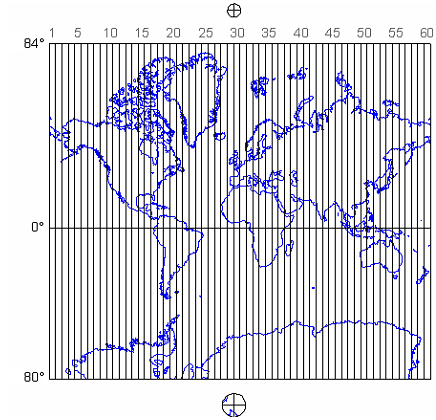
\includegraphics[width=\linewidth]{figures/ch2-fig8.png}
        \caption{Illustration of the 60 UTM zones dividing the Earth's surface, each spanning
                 6° of longitude. Polar regions beyond 84°\,N and 80°\,S are
                 excluded and covered by separate polar coordinate systems.}
        \label{fig:utm_zones_world}
    \end{subfigure}
    \hfill
    \begin{subfigure}[t]{0.42\textwidth}
        \centering
        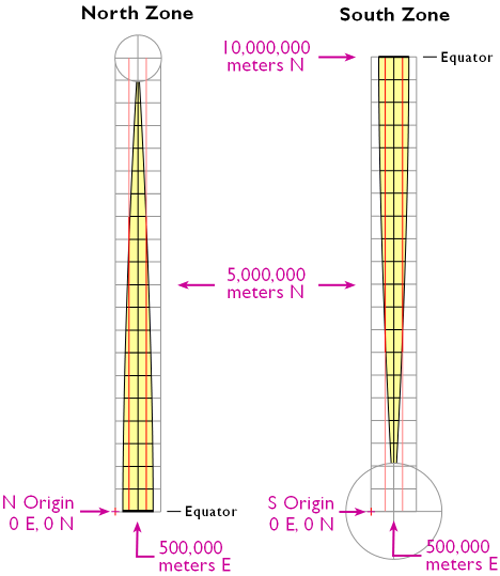
\includegraphics[width=\linewidth]{figures/UTM_Coordinate.png}
        \caption{Structure of a single UTM zone. Each zone spans 6° of
                 longitude and is subdivided into a north and south half at
                 the equator. Origins are placed 500{,}000\,m west of the
                 central meridian so that all coordinates within the zone are
                 positive.}
        \label{fig:utm_zone_detail}
    \end{subfigure}
    \caption[UTM coordinate overview]{The \ac{UTM}
             projects geographic (spherical) coordinates onto a planar
             Cartesian grid.
             Figures from \textcite{DiBiase_PennState_GEOG160},
             licensed under CC~BY-NC-SA~4.0.}
    \label{fig:utm_overview}
\end{figure}



\begin{comment}
    
\begin{figure}[htbp]
    \centering
    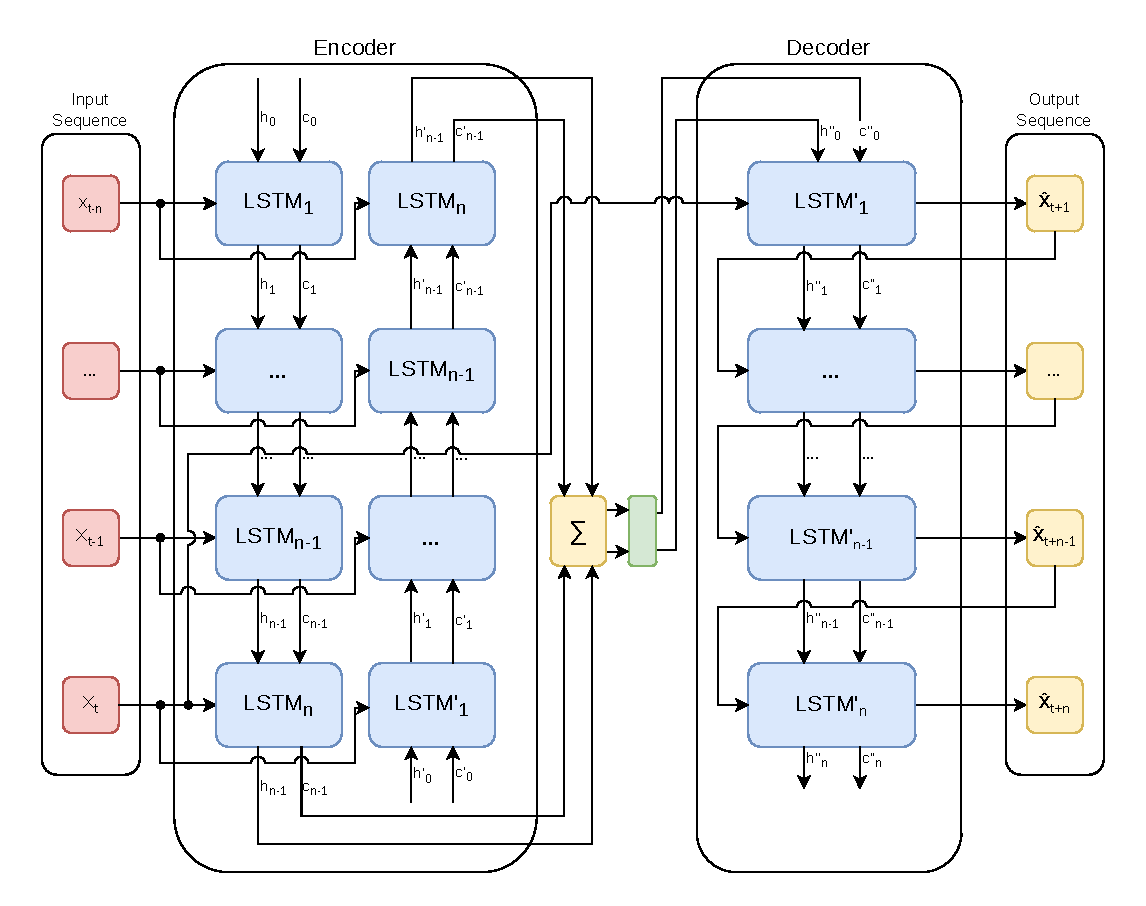
\includegraphics[width=0.75\linewidth]{figures/S2S_Bi-LSTM.drawio (1).pdf}
    \caption{Architecture utilizing a Bi-LSTM Encoder with a standard LSTM Decoder.}
    \label{fig:s2s_bilstm_appendix}
\end{figure}

\begin{figure}[htbp]
    \centering
    % \includegraphics[width=0.75\linewidth]{figures/S2S_Attention.drawio.pdf}
    \todo{wenn ich zeit für sowas habe. nachdem ich mich für architektur entschieden habe, diese hier rein}
    \caption{Sequence-to-Sequence architecture incorporating an Attention mechanism.}
    \label{fig:s2s_attention_appendix}
\end{figure}
\end{comment}







\begin{comment} %verison ohne resampling
    
% Seite 1: Folien 1–3
\begin{figure}[p]
    \centering
    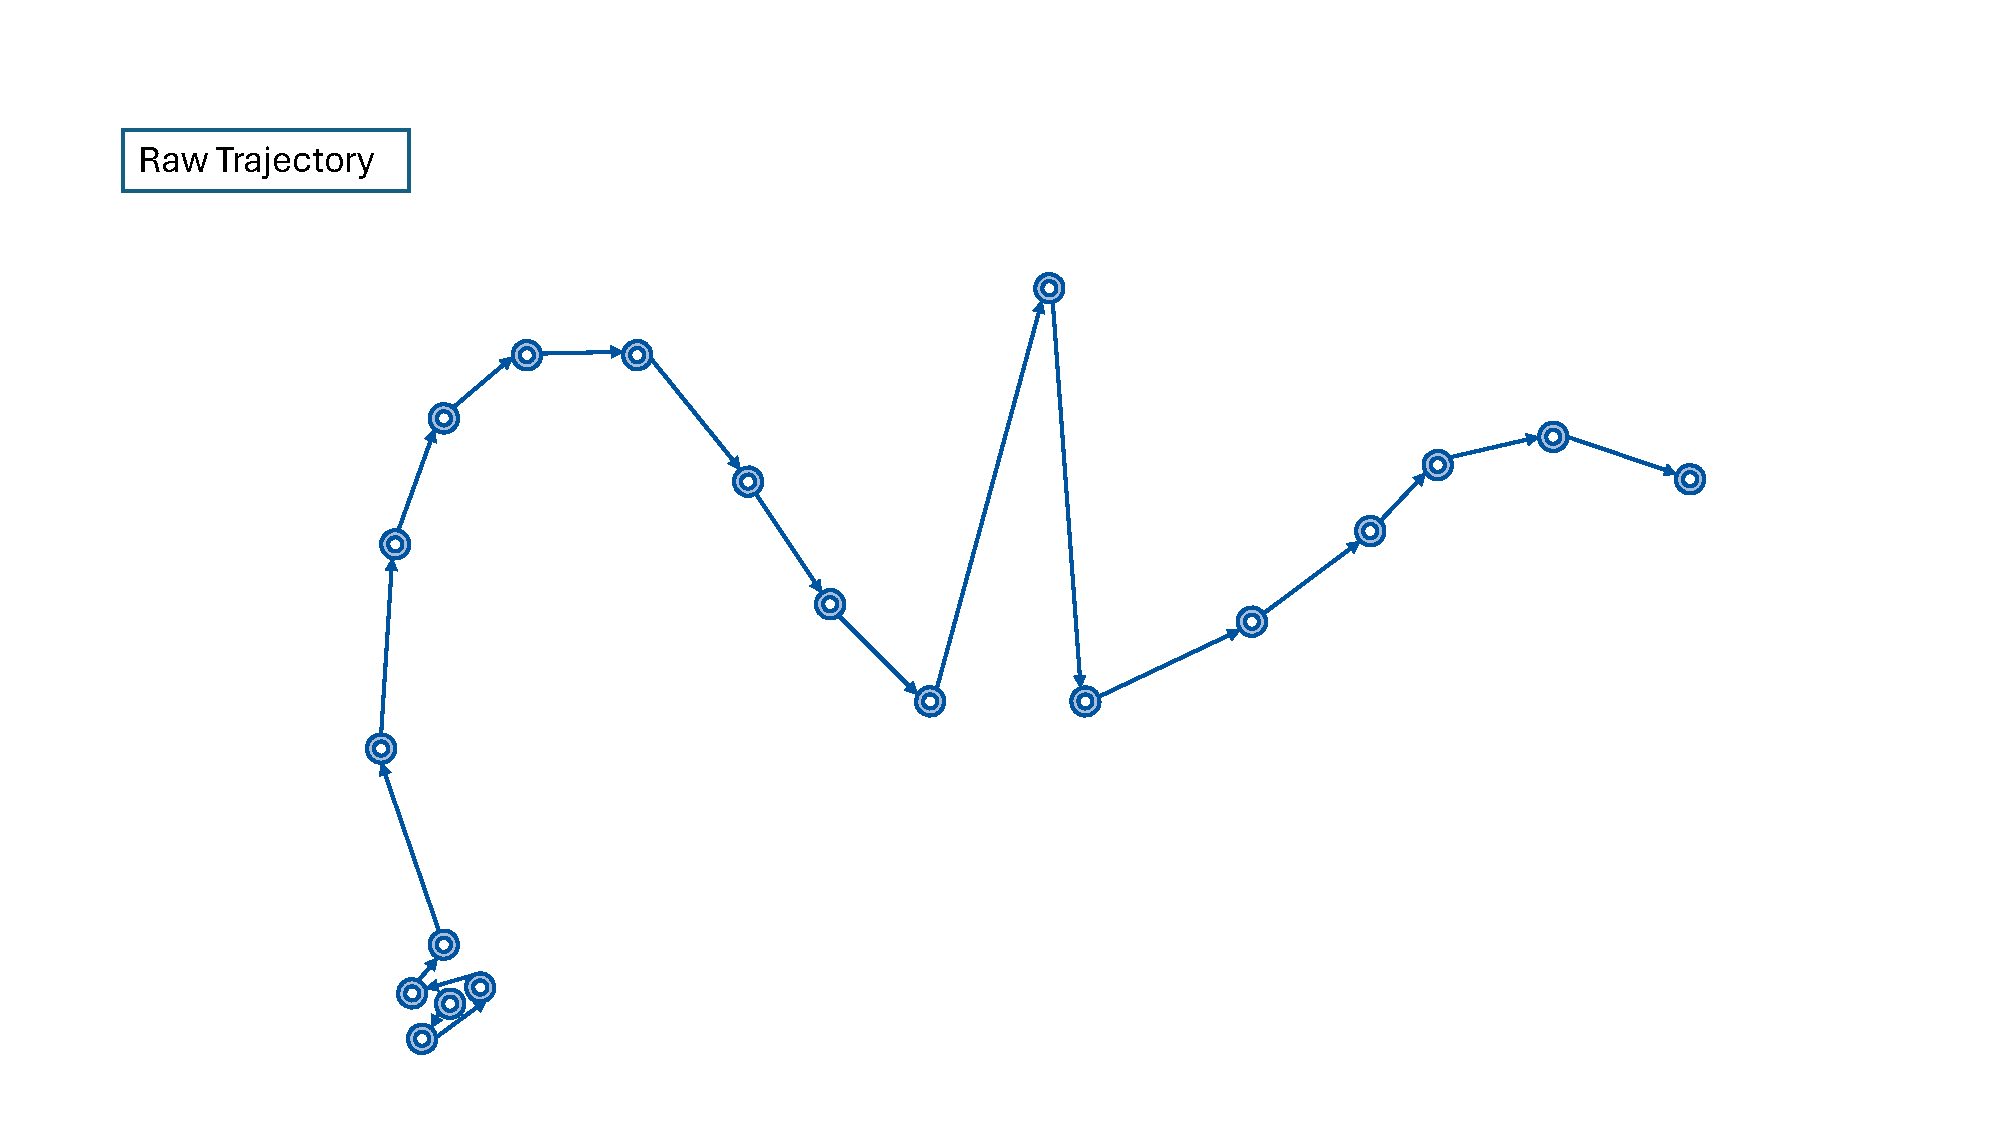
\includegraphics[height=0.32\textheight, page=1]{figures/Animation Preprocessing.pdf}\\[4pt]
    \includegraphics[height=0.32\textheight, page=2]{figures/Animation Preprocessing.pdf}\\[4pt]
    \includegraphics[height=0.32\textheight, page=3]{figures/Animation Preprocessing.pdf}
    \caption{Track Segmentation (1/2)}
    \label{fig:preprocessing-a}
\end{figure}

% Seite 2: Folien 4–5
\begin{figure}[p]
    \ContinuedFloat
    \centering
    \includegraphics[height=0.32\textheight, page=4]{figures/Animation Preprocessing.pdf}\\[4pt]
    \includegraphics[height=0.32\textheight, page=5]{figures/Animation Preprocessing.pdf}
    \caption{Track Segmentation (2/2)}
    \label{fig:preprocessing-b}
\end{figure}
%nochmla
\end{comment}

% Seite 1: Folien 1–3
\begin{figure}[p]
    \centering
    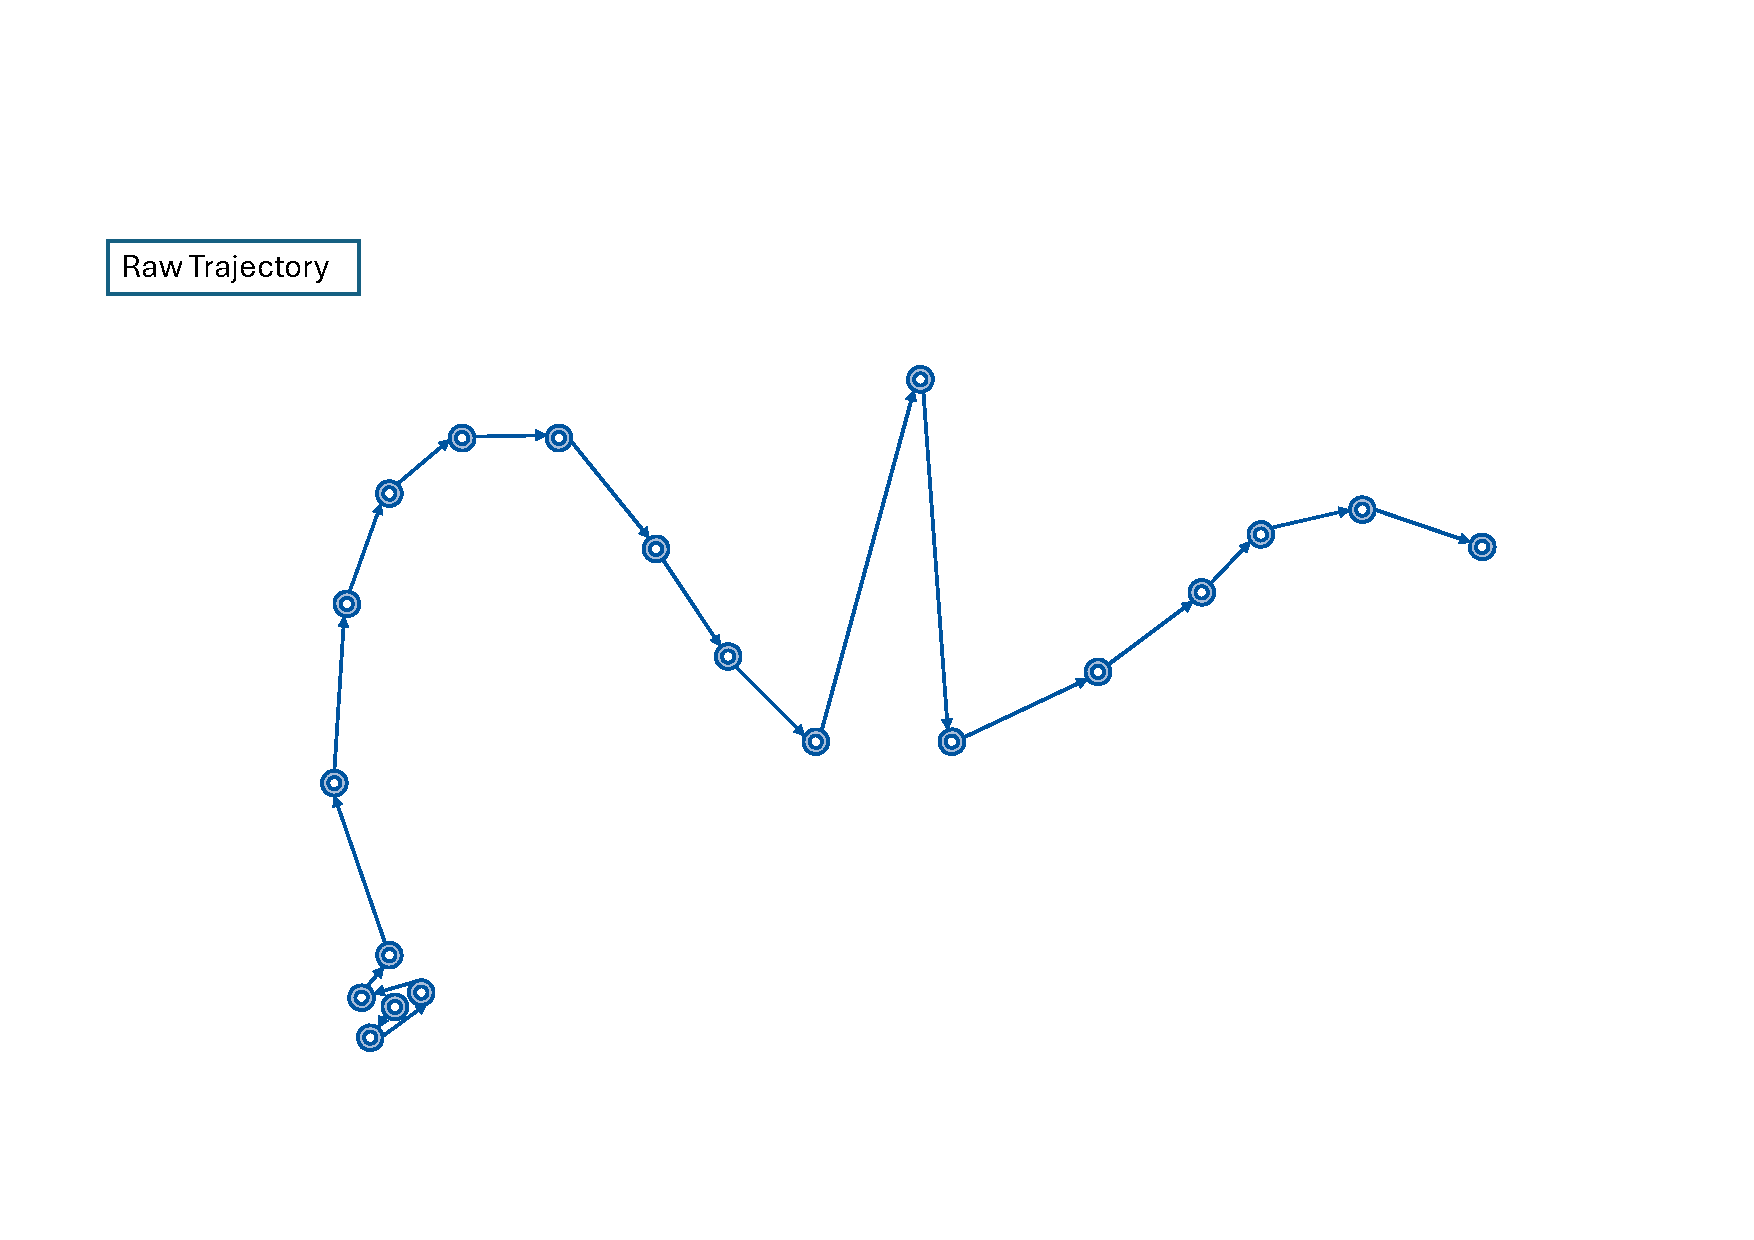
\includegraphics[height=0.32\textheight, page=1]{figures/animationpreprocessingwithsampling.pdf}\\[4pt]
    \includegraphics[height=0.32\textheight, page=2]{figures/animationpreprocessingwithsampling.pdf}\\[4pt]
    \includegraphics[height=0.32\textheight, page=3]{figures/animationpreprocessingwithsampling.pdf}
    \caption[Preprocessing visualisation (1/2)]{Preprocessing visualisation. First, implausible messages are removed. The remaining trajectories are then resampled to a fixed 30 s grid. After resampling, a sliding window is applied to extract the final samples. (1/2)}
    \label{fig:preprocessing-a}
\end{figure}

% Seite 2: Folien 4–7
\begin{figure}[p]
    \ContinuedFloat
    \centering
    \includegraphics[height=0.32\textheight, page=4]{figures/animationpreprocessingwithsampling.pdf}\\[4pt]
    \includegraphics[height=0.32\textheight, page=5]{figures/animationpreprocessingwithsampling.pdf}\\[4pt]
    \includegraphics[height=0.32\textheight, page=6]{figures/animationpreprocessingwithsampling.pdf}\\[4pt]
    %\includegraphics[height=0.32\textheight, page=7]{figures/animationpreprocessingwithsampling.pdf}\\[4pt]

    %letzt folie nicht ultra wichtig

    \caption[Preprocessing visualisation (2/2)]{Preprocessing visualisation. First, implausible messages are removed. The remaining trajectories are then resampled to a fixed 30 s grid. After resampling, a sliding window is applied to to extract the final samples. (2/2)}
    \label{fig:preprocessing-b}
\end{figure}
%nochmla



\begin{figure}[h]
    \centering
    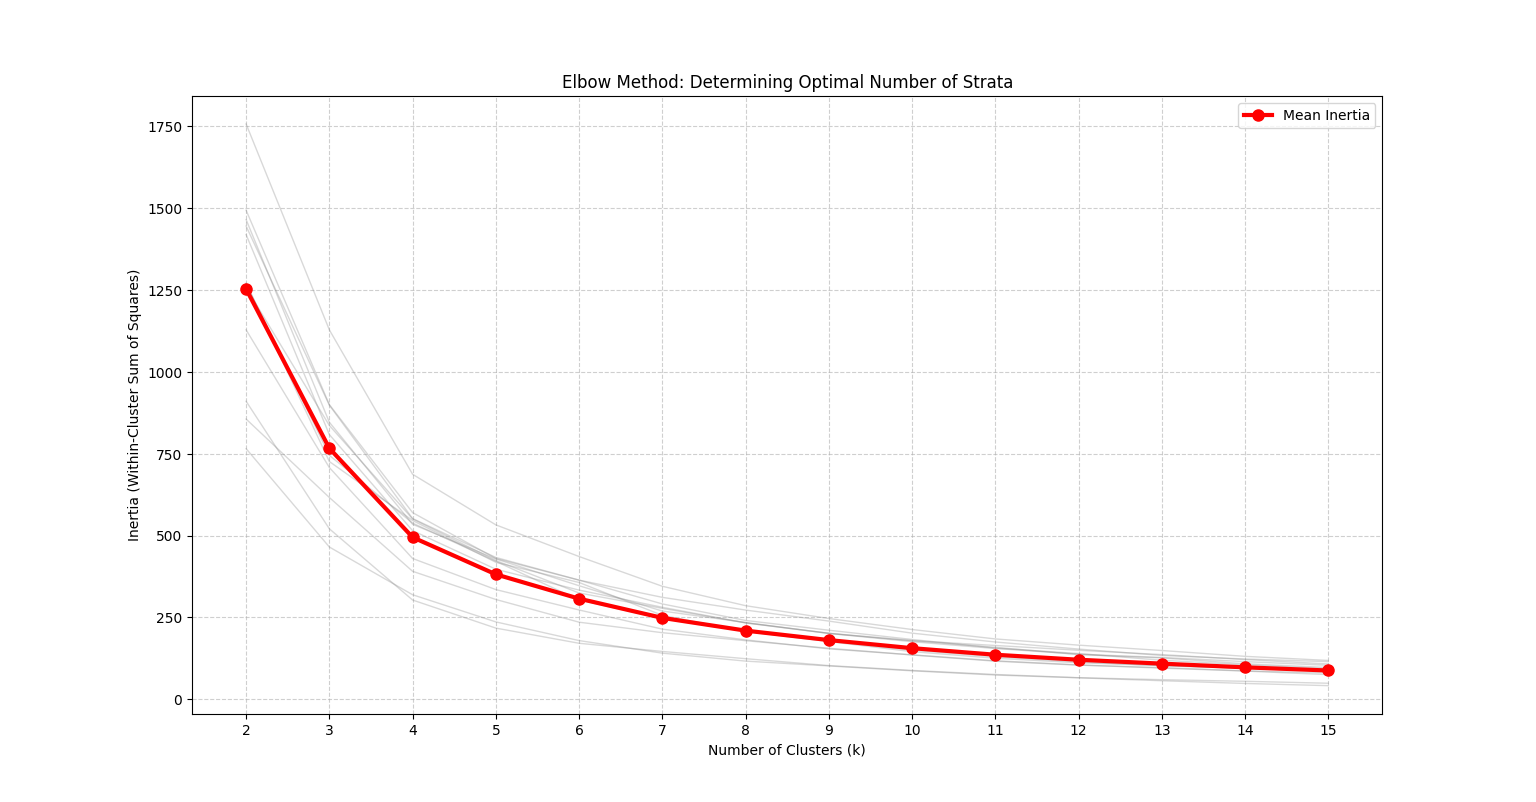
\includegraphics[width=1\linewidth,trim=0 8 0 70,clip]{figures/elbow_strat.png}
    \caption[Strata Elbow-Plot]{Elbow-Plot: Inertia vs. Number of Clusters $k \in [2, 15]$ used to estimate the optimal number of strata. For each file in the sampled dataset, vessel profiles were aggregated by computing mean \acf{SOG}, maximum absolute \acf{ROT}, and the context label. Features were standardised prior to clustering. KMeans ($n\_init=10$) was fitted independently per file; grey lines represent per-file inertia curves, the red line indicates the mean across all files. The elbow between $k=4$ and $k=5$ justifies the choice of five strata to capture the kinematic diversity of the dataset.}
    
    \label{fig:elbow_strat}
\end{figure}

\begin{comment}
\begin{figure}[h]
    \centering
    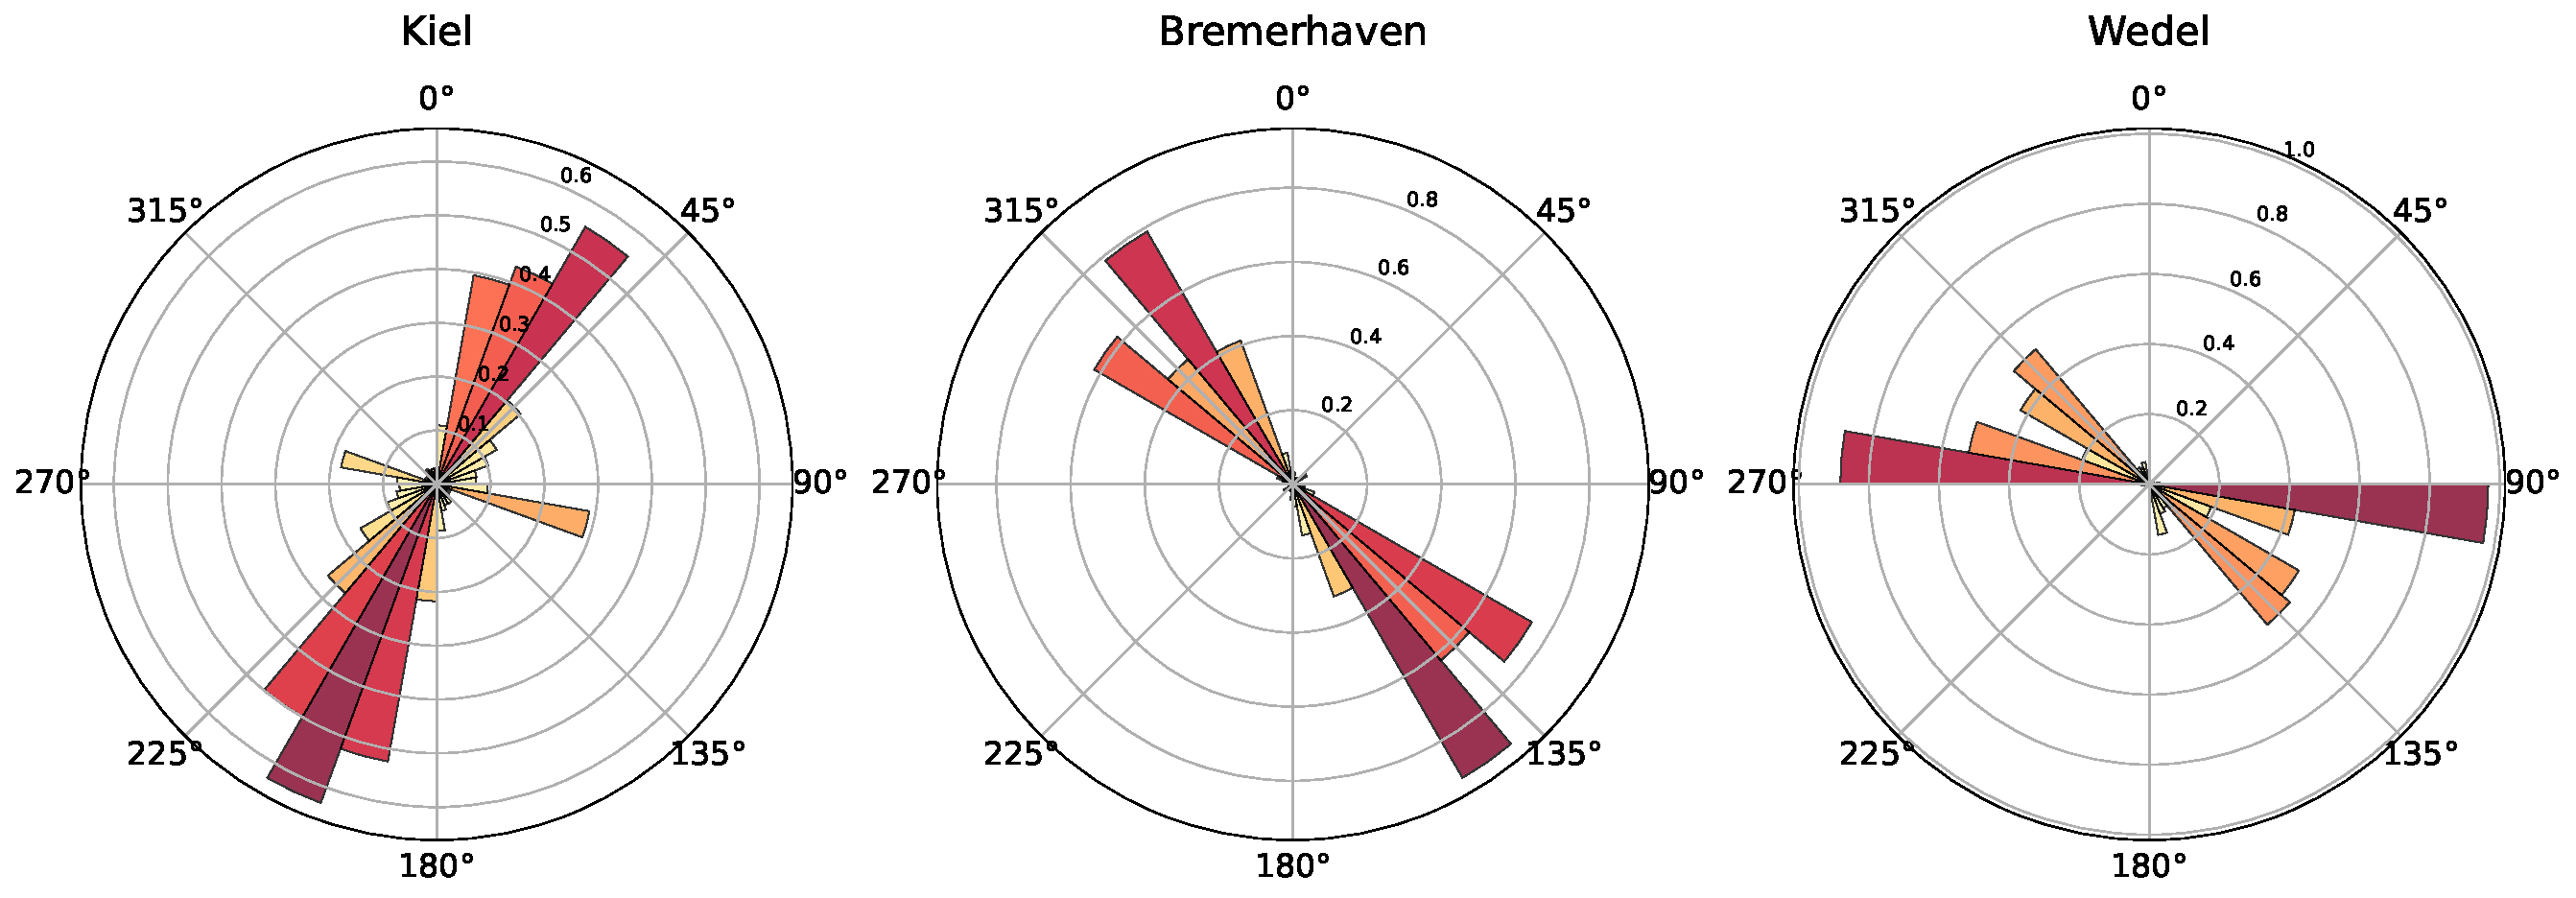
\includegraphics[width=0.85\linewidth]{figures/cog_polar_heatmap.pdf} %\todo
    \caption[COG Polar Histogram]{Polar Histogram of Vessel \acf{COG} after the Preprocessing Pipeline \todo{bigger labels orcut of the top and write Kiel left, bremerhaven middle wedel right}}
    \label{fig:polarhist}
\end{figure}
\end{comment}

\begin{figure}[h]
    \centering
    \begin{subfigure}[b]{0.95\linewidth}
        \centering
        % trim=left bottom right top. Increase the last value to cut more from the top.
        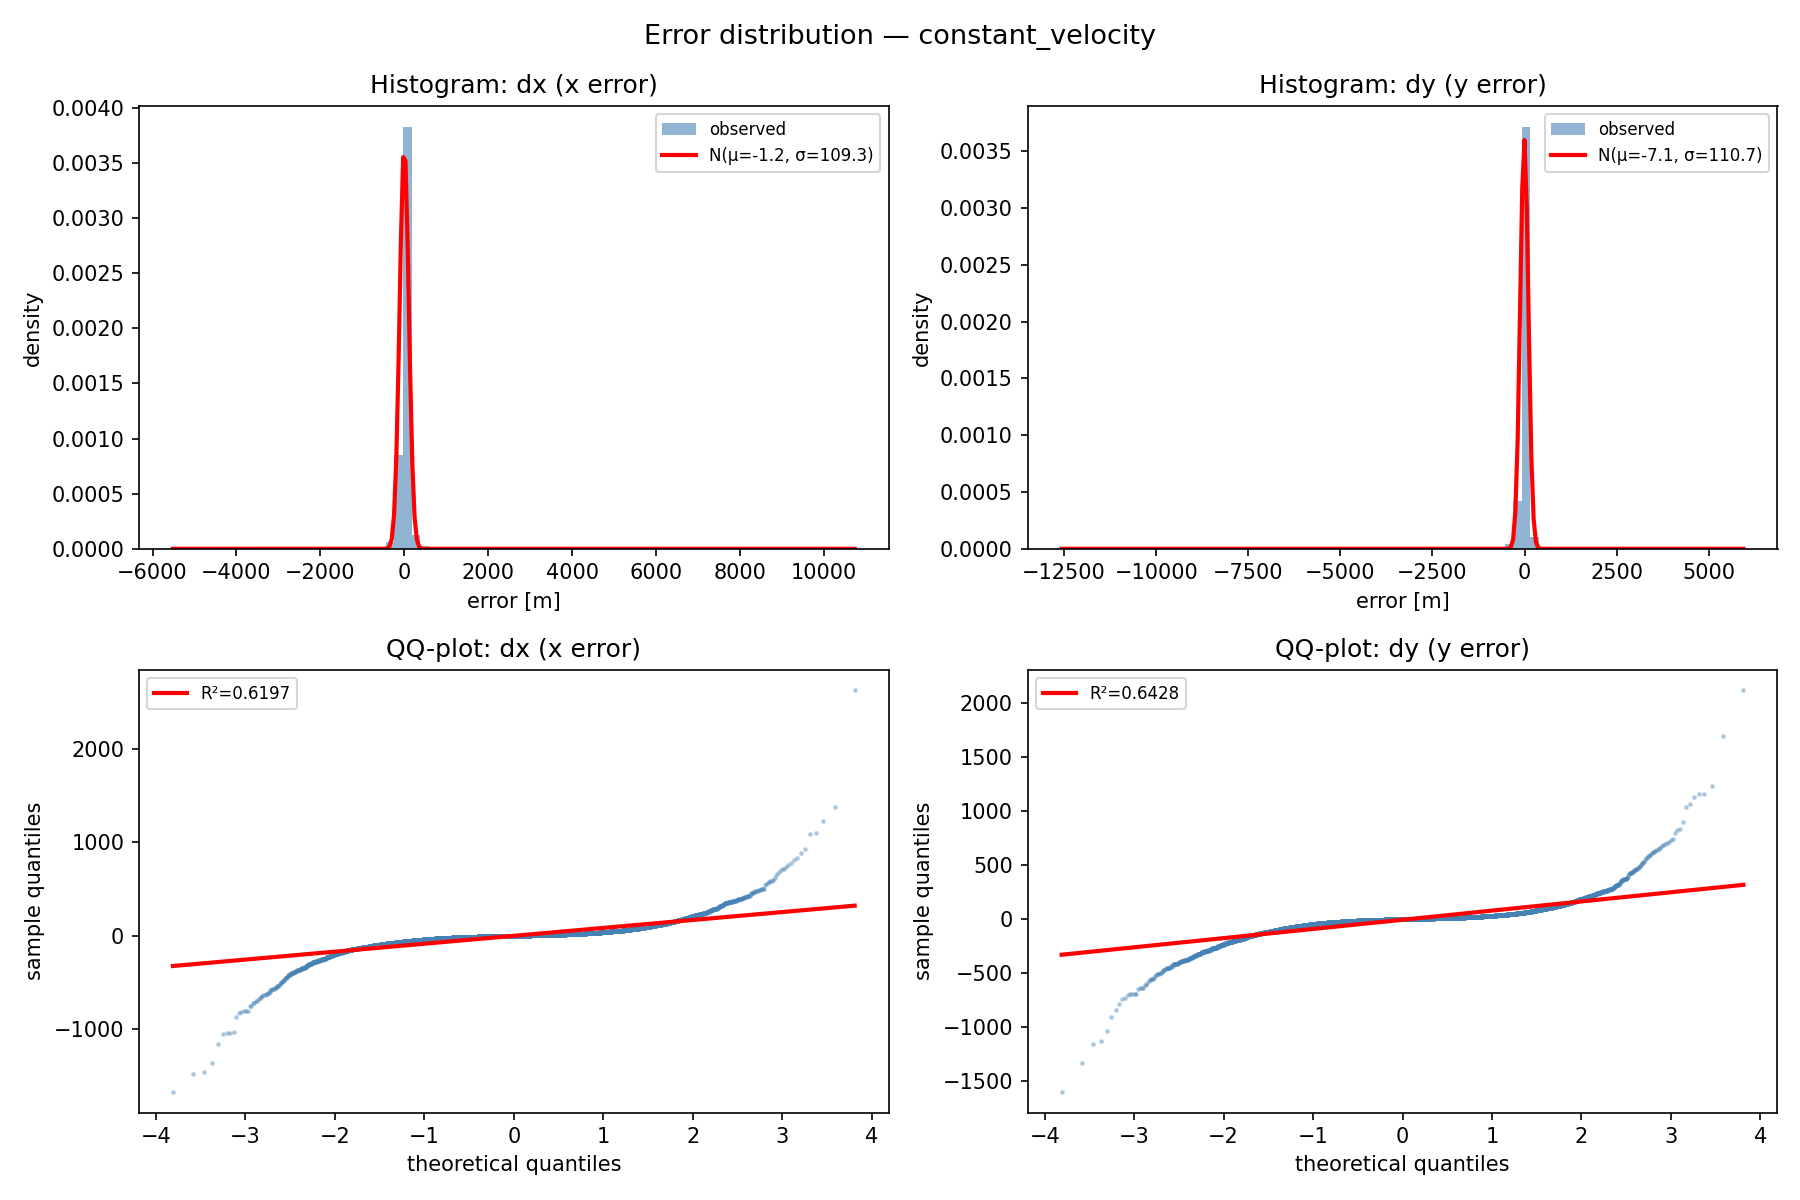
\includegraphics[width=\linewidth, trim=0cm 0cm 0cm 105mm, clip]{figures/error_distribution_constant_velocity.png}
        \caption{\acs{CV}}
        \label{fig:qqplot_cv}
    \end{subfigure}
    
    \vspace{1em} % Adds a bit of vertical space between the top and bottom plots
    
    \begin{subfigure}[b]{0.95\linewidth}
        \centering
        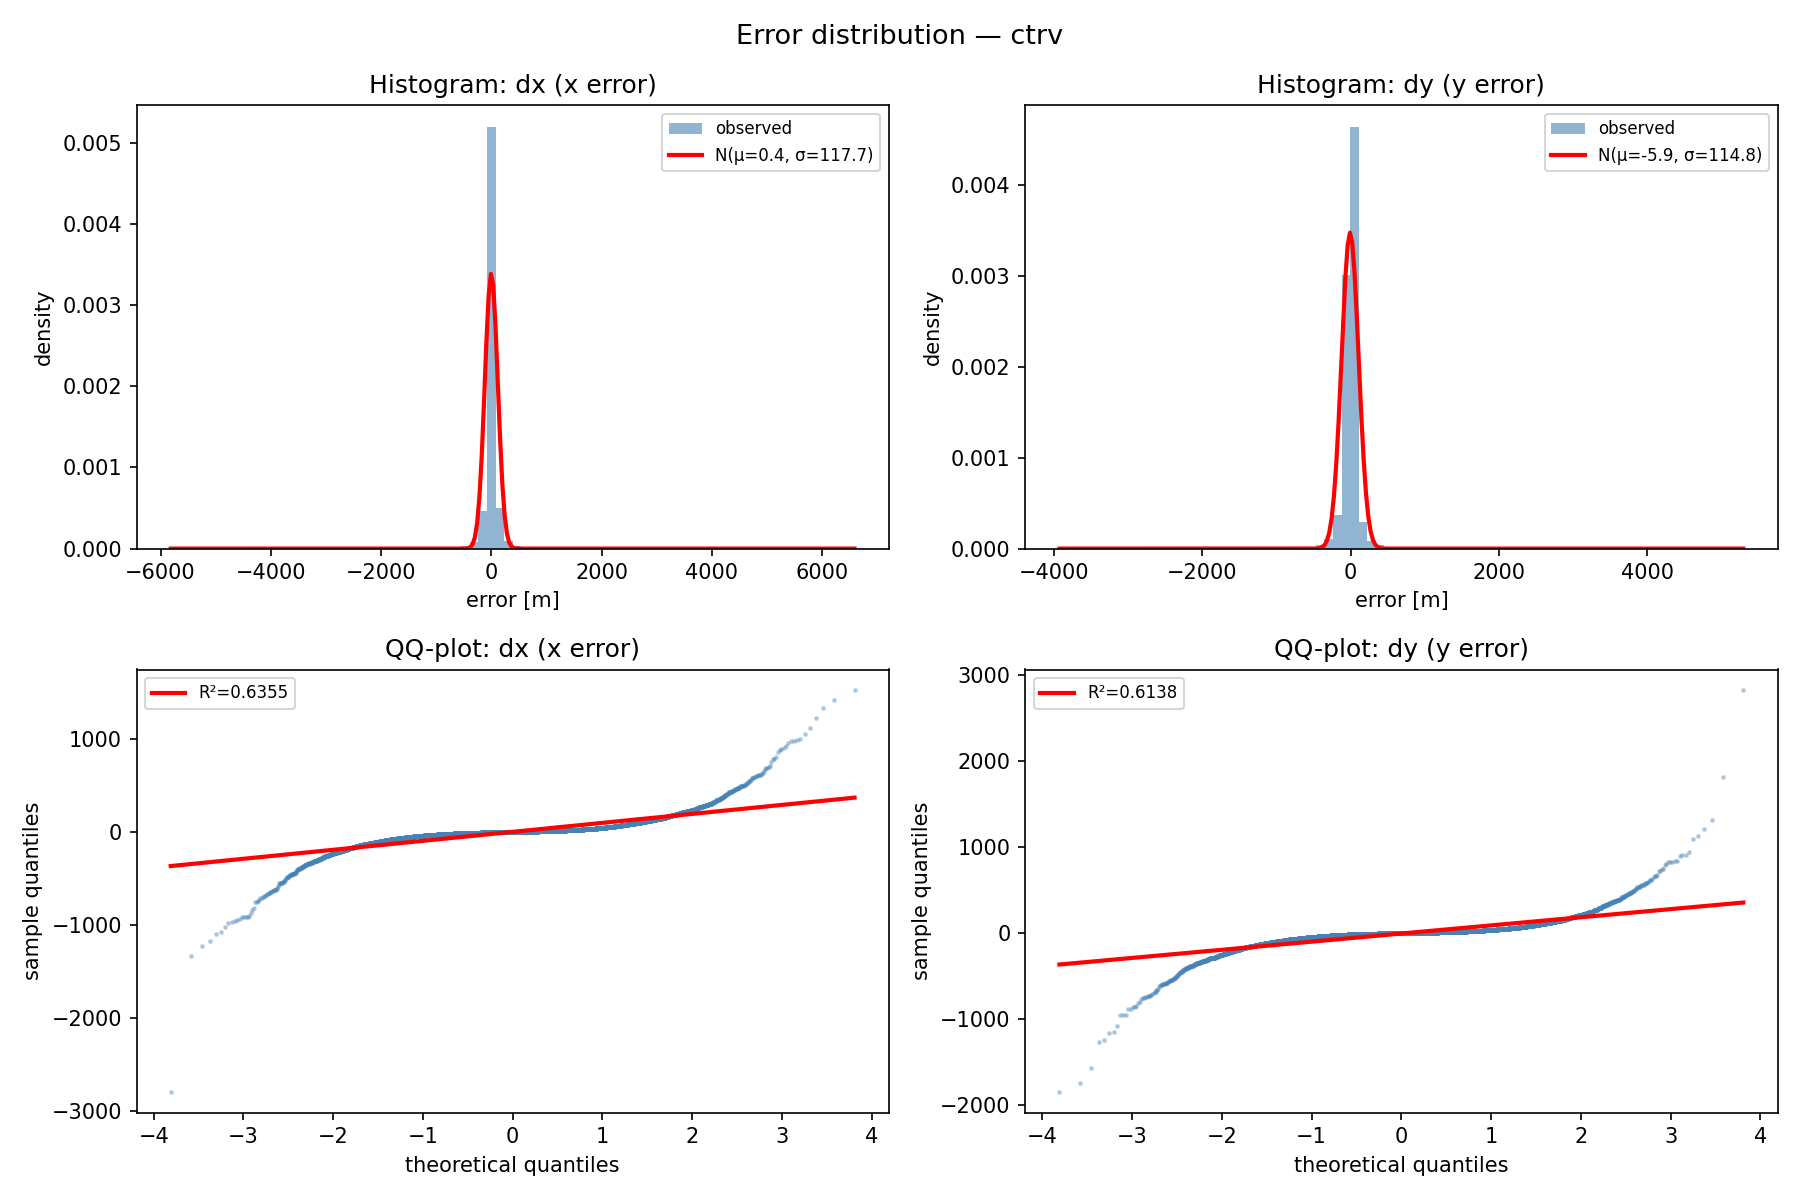
\includegraphics[width=\linewidth, trim=0cm 0cm 0cm 105mm, clip]{figures/error_distribution_ctrv.png}
        \caption{\acs{CTRV}}
        \label{fig:qqplot_ctrv}
    \end{subfigure}
    
    \caption[CV and CTRV QQ-Plot]{    
    Quantile-Quantile (QQ) plots of the positional prediction errors ($dx$ and $dy$) for \acf{CV} and \acf{CTRV} models. The errors of these pure kinematic models represent the real process noise of the \acp{KF}' underlying motion models, %plural
    which they internally model as a Gaussian distribution. The solid red lines represent the theoretical normal distribution; the significant deviation of the sample quantiles at the extremes indicates heavy tails and extreme outliers. This is supported by low coefficient of determination ($R^2$) values ranging from 0.6138 to 0.6428, demonstrating a clear violation of the Gaussian noise assumption.}
    \label{fig:qqplot}
\end{figure}


\begin{figure}
    \centering
    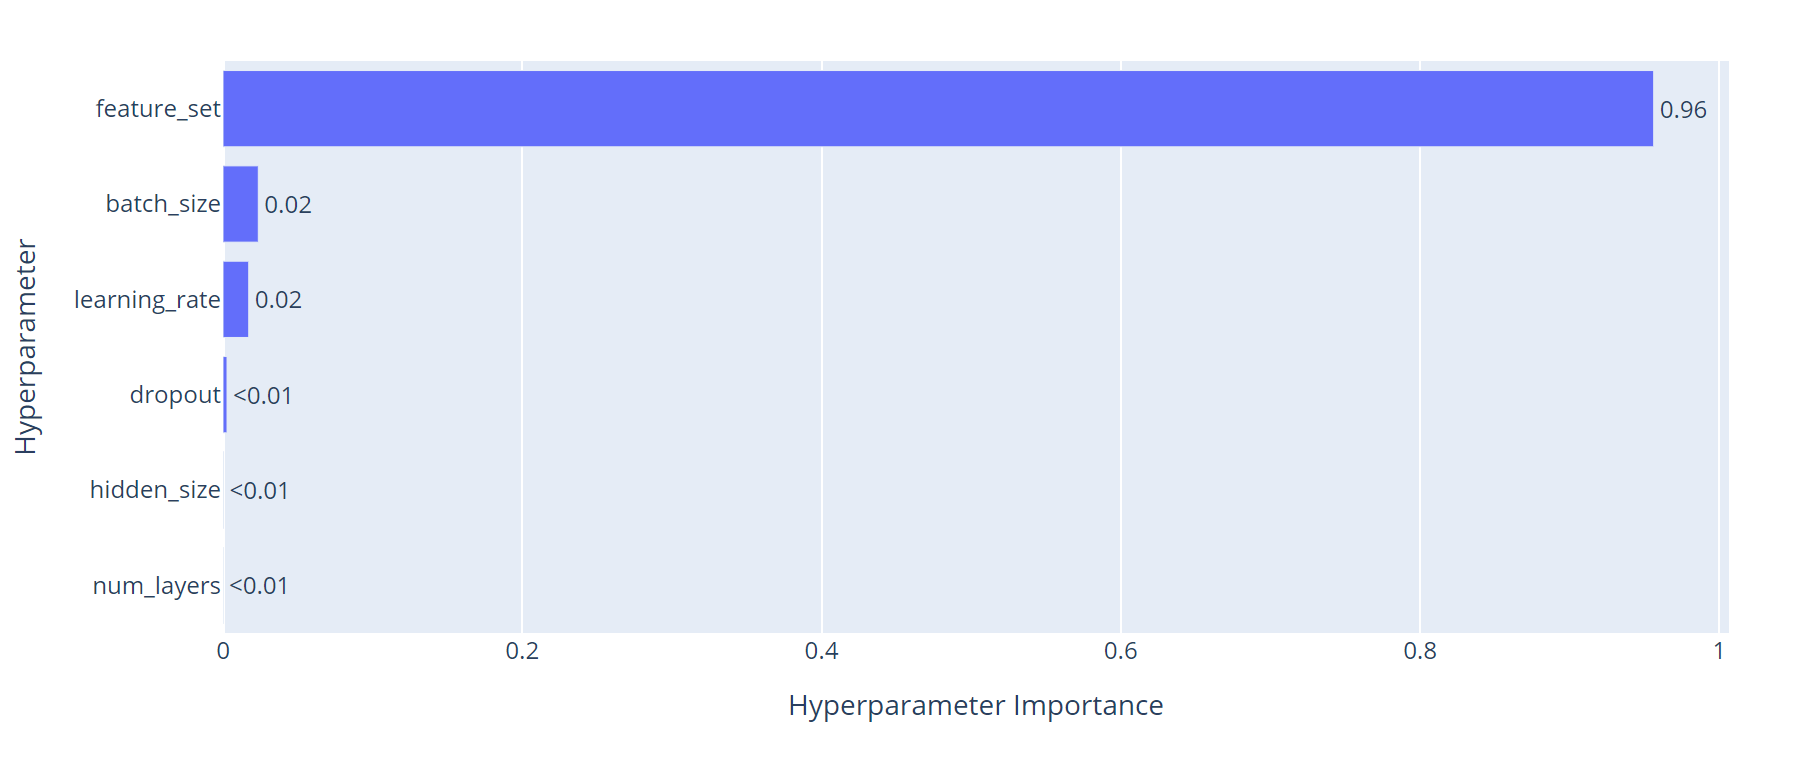
\includegraphics[width=0.95\linewidth]{figures/lstmhp.png}
    \caption[Hyperparameter Importances for the LSTM]{Quantitative hyperparameter importances for the \acf{LSTM}, calculated by Optuna using the \acf{fANOVA} framework. fANOVA isolates the marginal contribution of each parameter to the overall variance of the objective function, and thus provides quantitative metrics. The \texttt{feature\_set} dominates convergence success of the model by a significantly large margin. This high score must be interpreted with caution, as it is amplified by the evaluation bias detailed in Section \ref{lim:prior}. Conversely, \texttt{hidden\_size} registers an extremely low importance score; this matches with the observations from the parallel coordinate plot (Figure \ref{fig:paralelcord}), which demonstrated that exploring a wide range of hidden sizes had little to no impact on the final performance. Notably, \texttt{num\_layers} yields an importance of zero strictly because it was held constant and not defined as an active variable in this tuning space.}
    \label{fig:lstmhpimportances}
\end{figure}






\begin{comment}
\todo {weg mit den zweien die haben keinen mehrwert außer schau mal, eine statistik. außerdem istmissisipi noch drin}
\begin{figure}[ht]
\centering
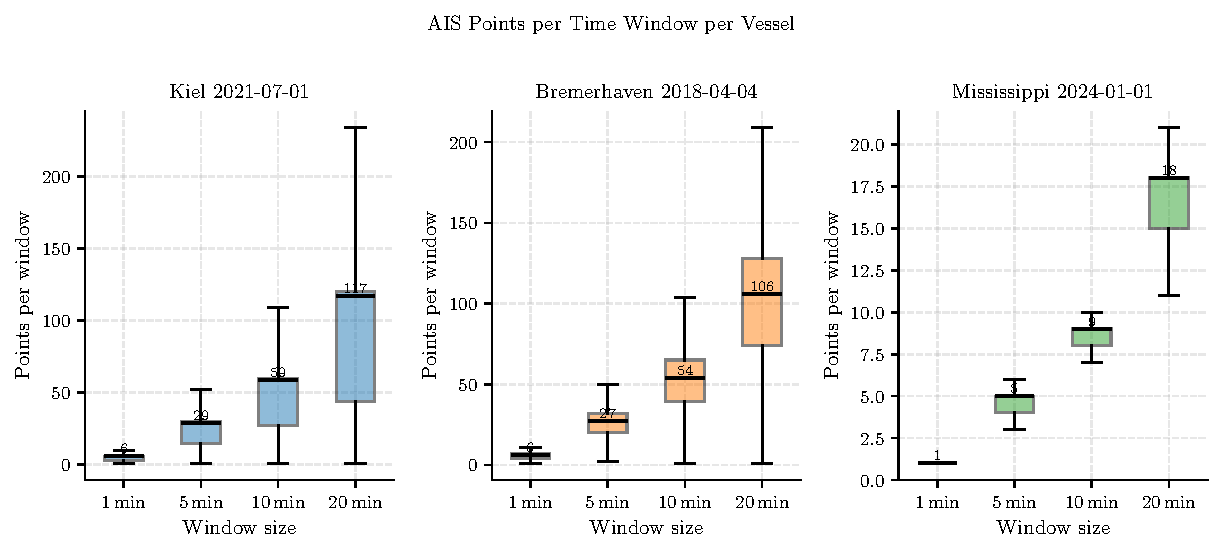
\includegraphics[width=1\textwidth]{figures/points_per_window.pdf}
\caption{Boxplot of AIS points per time window per vessel (sample day per dataset).}
\label{fig:points-per-window}
\end{figure}


\begin{figure}[ht]
\centering
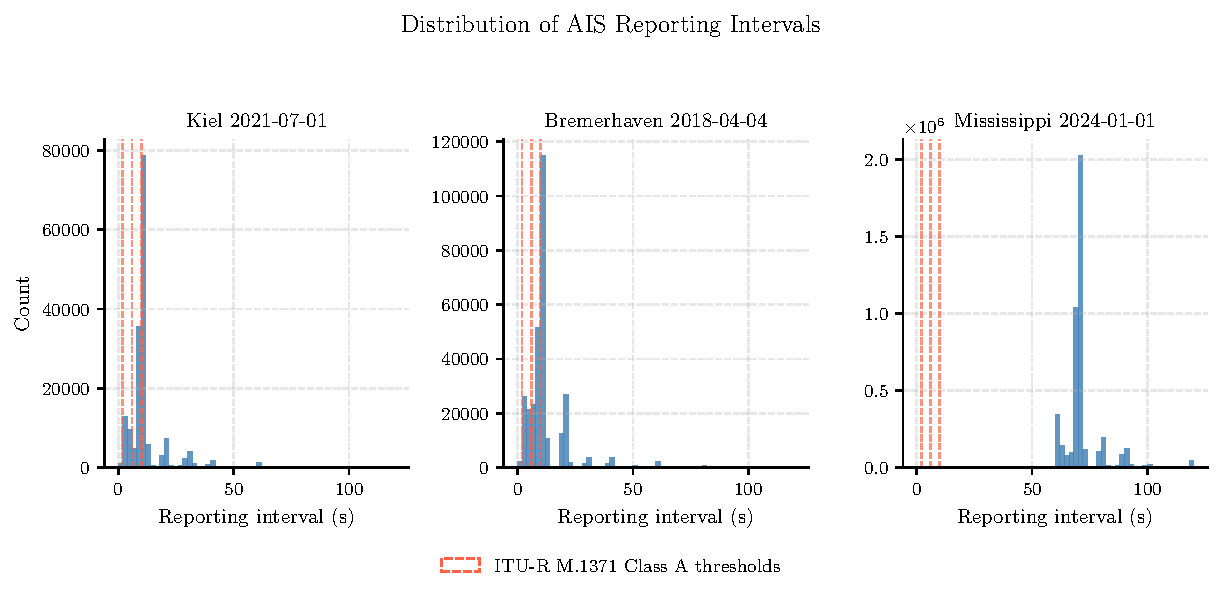
\includegraphics[width=1\textwidth]{figures/interval_hist.pdf}
\caption{Boxplot of inter-message intervals by velocity class.}
\label{fig:interval-hist}
\end{figure}
\end{comment}

%%%%%%sample trajectori4es

\FloatBarrier

% Optional: keep subfigure spacing tight
\captionsetup[subfigure]{justification=centering}

% =========================
% Domain 1 Channel
% =========================
\begin{figure}[p]
    \centering

    \begin{subfigure}[t]{0.6\textwidth}
        \centering
        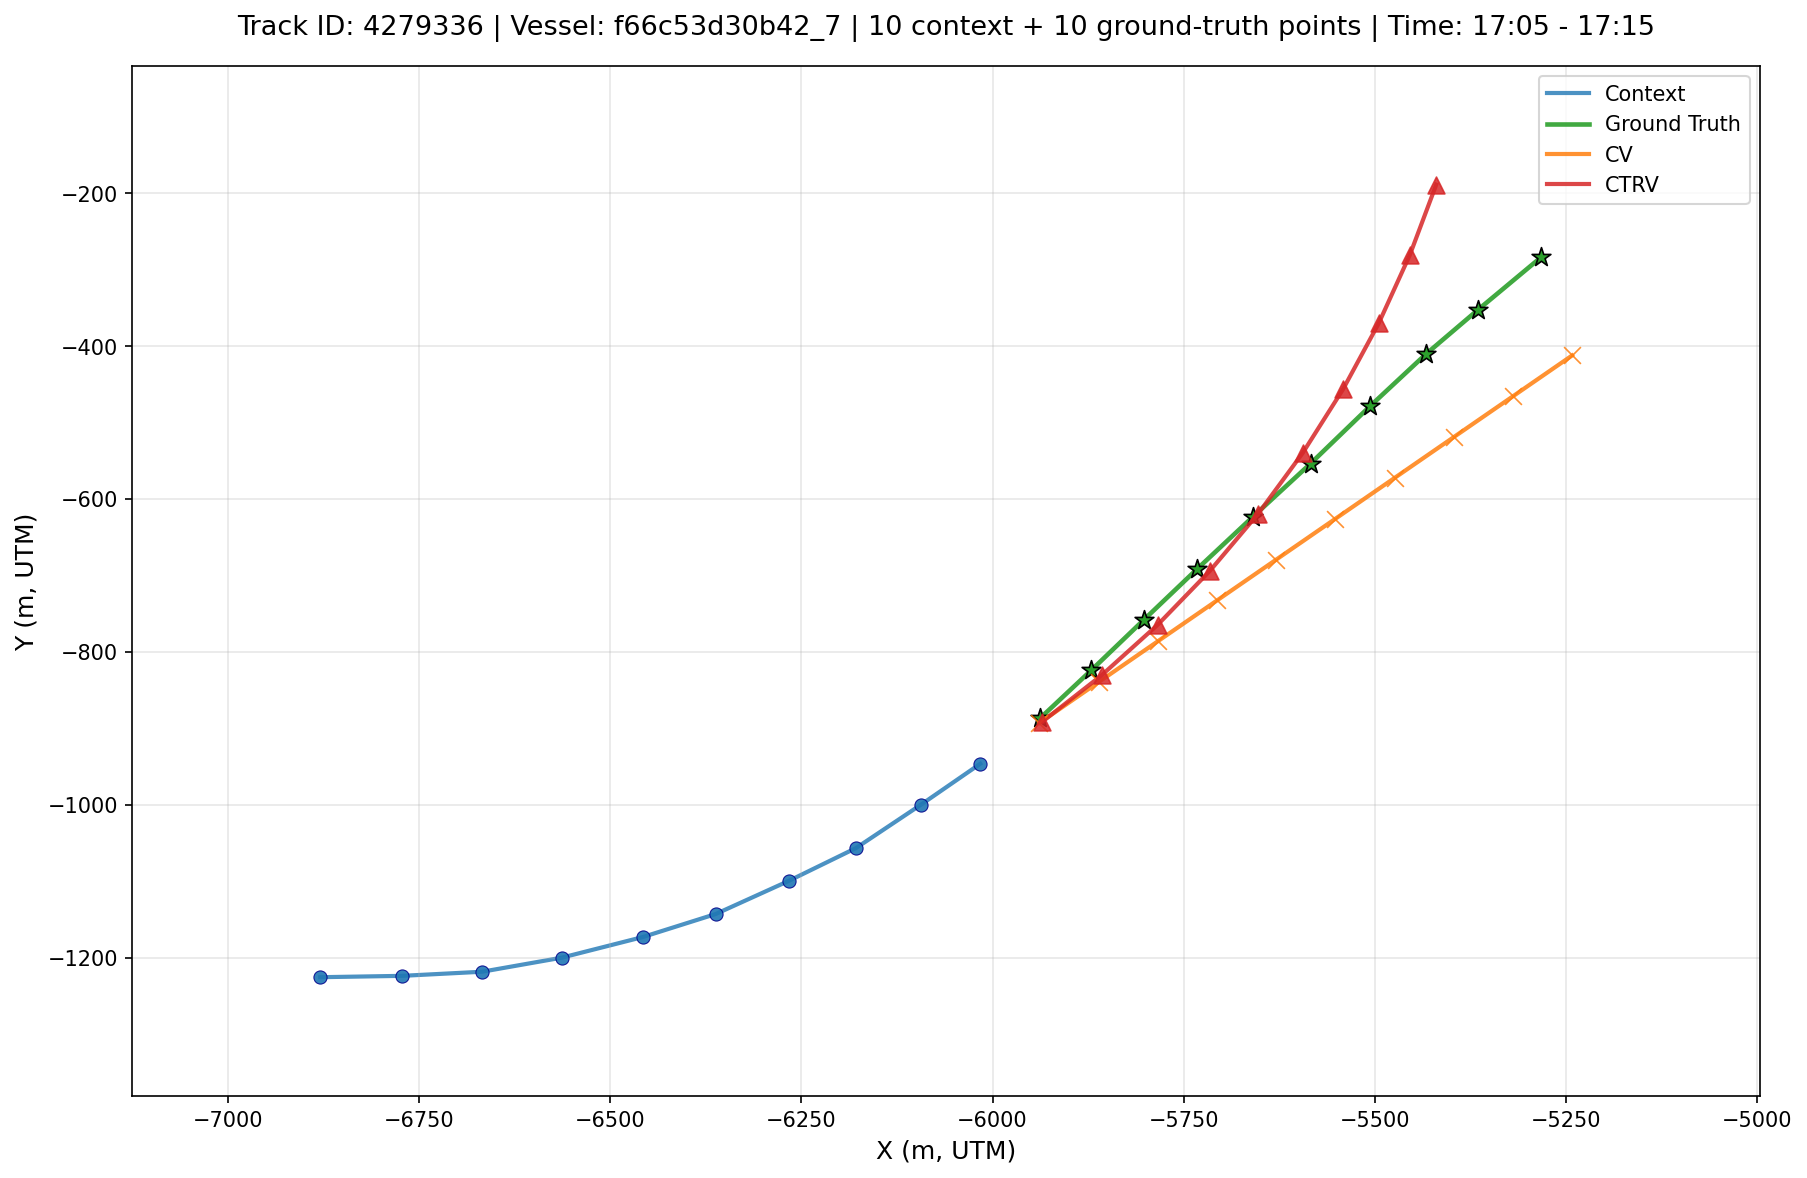
\includegraphics[width=\linewidth, trim=0 0 0cm 1.6cm,clip]{figures/domain11.png}
    \end{subfigure}

    \vspace{0.5em}

    \begin{subfigure}[t]{0.6\textwidth}
        \centering
        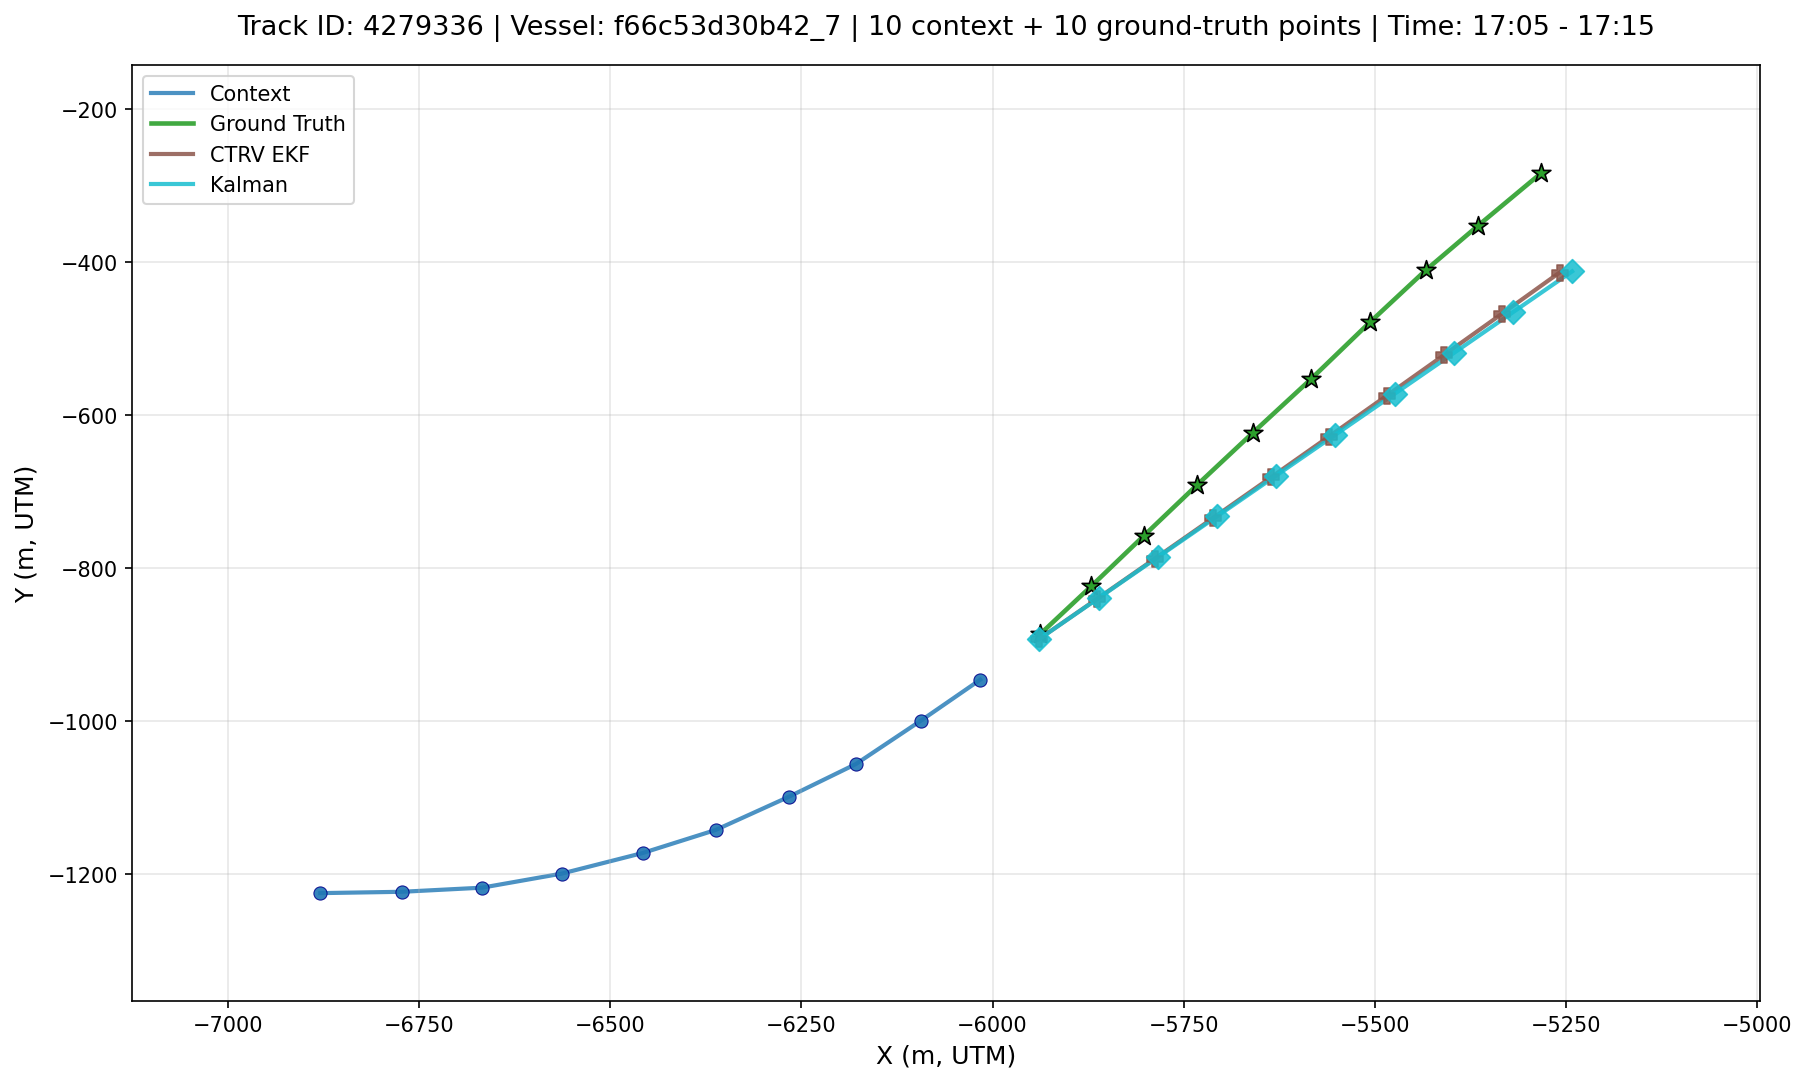
\includegraphics[width=\linewidth, trim=0 0 0cm 1.6cm,clip]{figures/domain12.png}
    \end{subfigure}

    \vspace{0.5em}

    \begin{subfigure}[t]{0.6\textwidth}
        \centering
        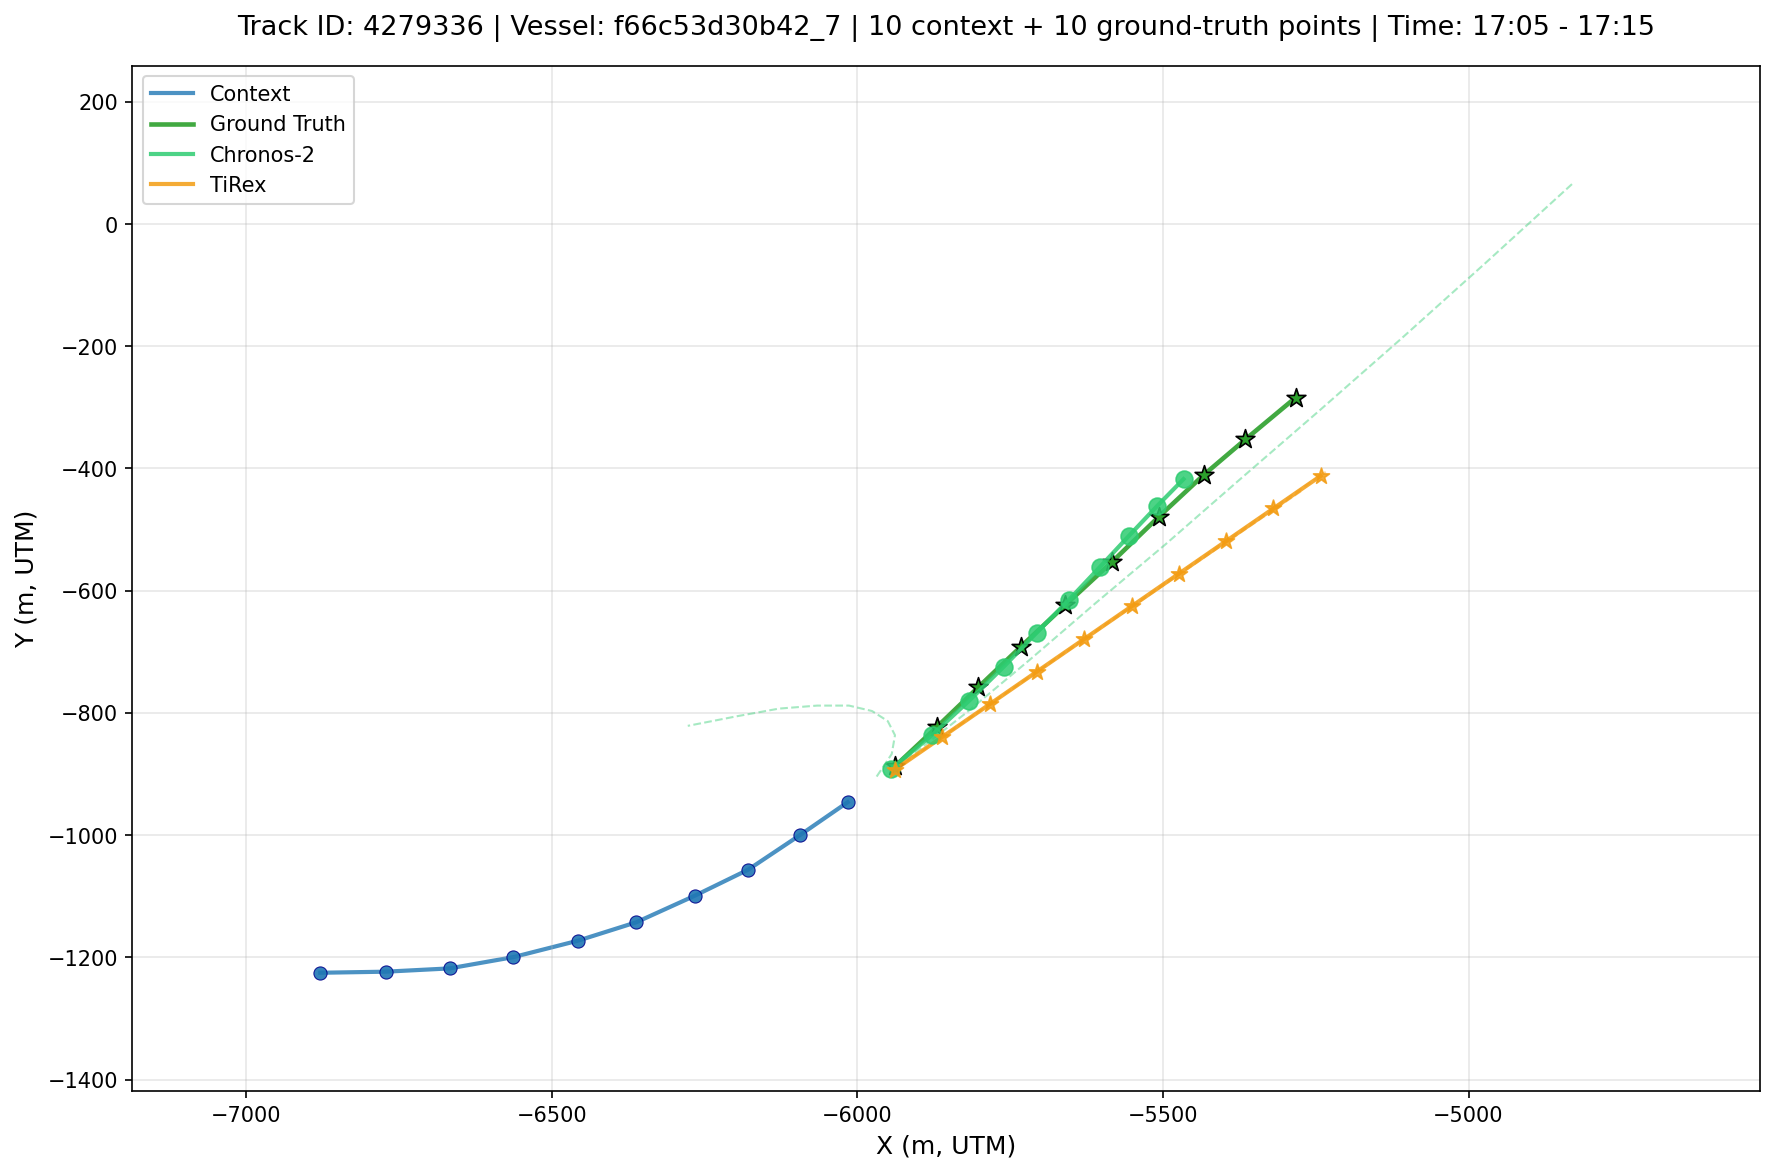
\includegraphics[width=\linewidth, trim=0 0 0cm 1.6cm,clip]{figures/domain13.png}
    \end{subfigure}

    \vspace{0.5em}

    \begin{subfigure}[t]{0.6\textwidth}
        \centering
        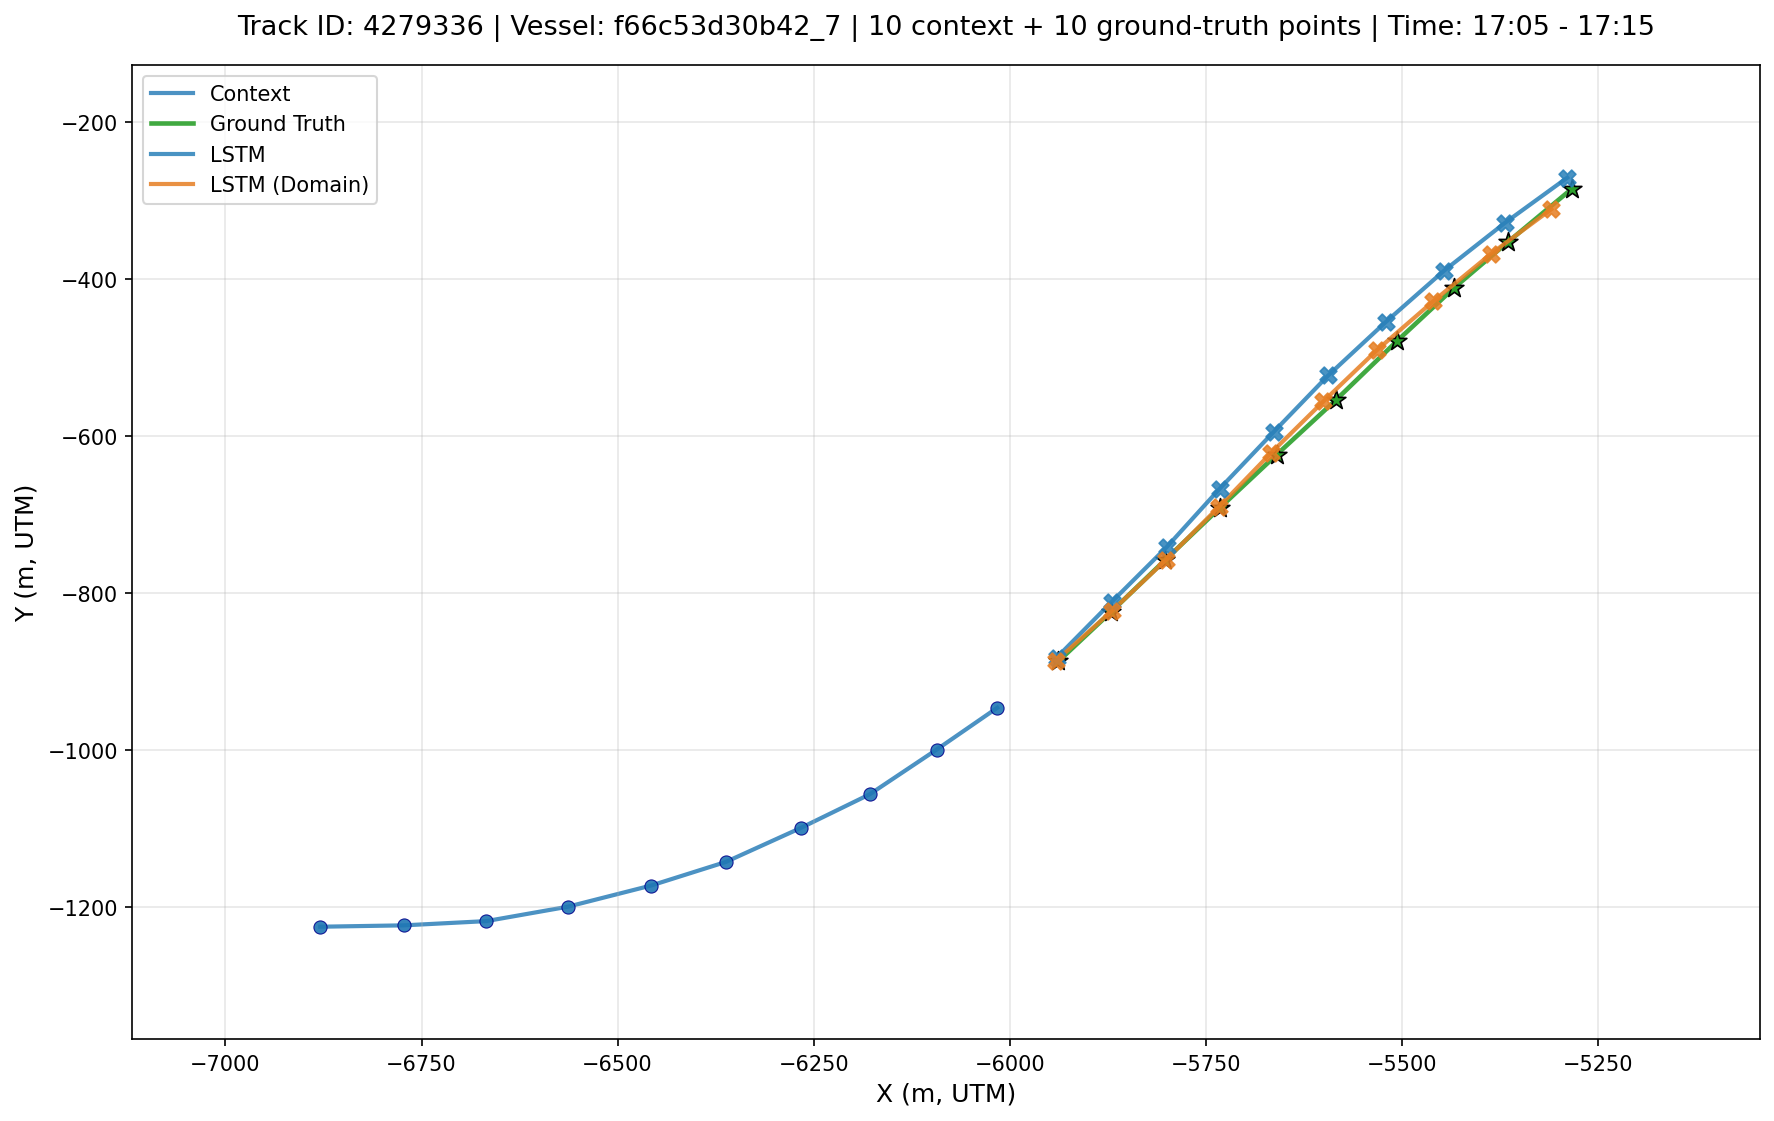
\includegraphics[width=\linewidth, trim=0 0 0cm 1.6cm,clip]{figures/domain14.png}
    \end{subfigure}


    \caption[Forecasting examples for Channel (Kiel)]{Forecasting examples for the Channel domain (Kiel). These plots provide a qualitative visual comparison of the predicted paths generated by the evaluated models. The observed context window is displayed in blue, while the actual ground truth trajectory that follows is marked with green stars. The various model predictions are shown in the remaining colours. For Chronos 2, the 80\% certainty band is displayed using thin green dots. Both axes represent relative \ac{UTM} coordinates measured in meters.}
    \label{fig:domain1}
\end{figure}

\FloatBarrier
\clearpage

% =========================
% Domain 2
% =========================
\begin{figure}[p]
    \centering

    \begin{subfigure}[t]{0.49\textwidth}
        \centering
        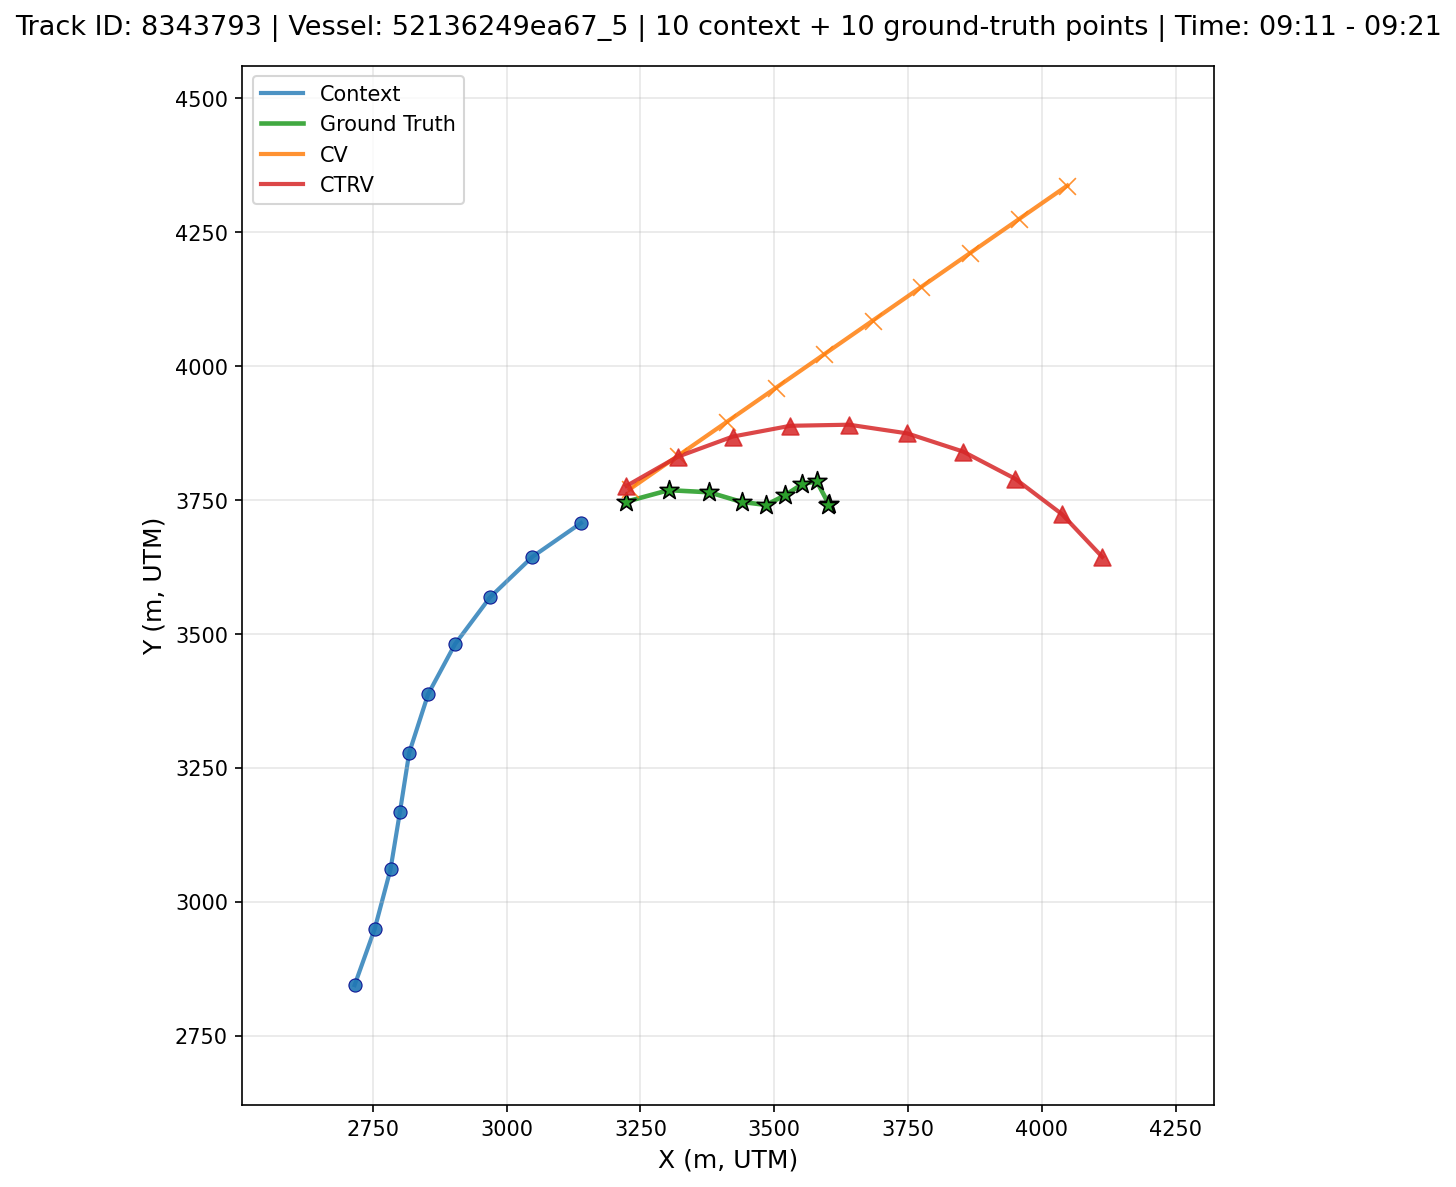
\includegraphics[width=\linewidth, trim=0 0 0cm 1.6cm,clip]{figures/domain21.png}
    \end{subfigure}
    \hfill
    \begin{subfigure}[t]{0.49\textwidth}
        \centering
        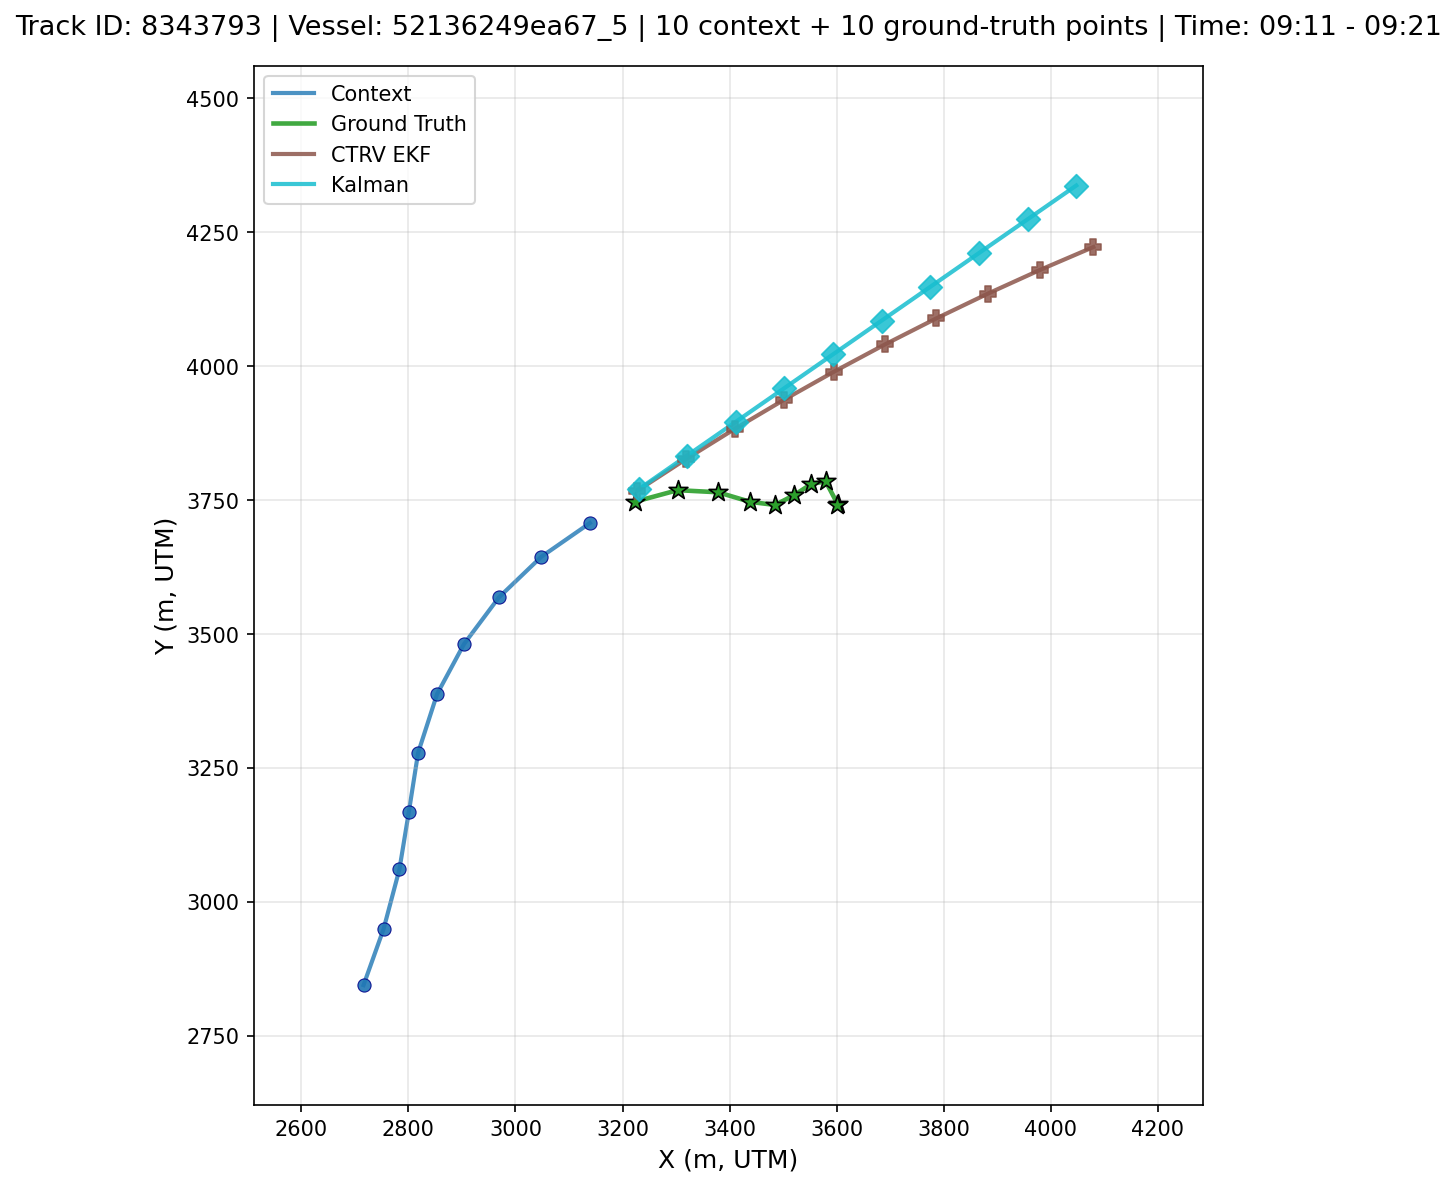
\includegraphics[width=\linewidth, trim=0 0 0cm 1.6cm,clip]{figures/domain22.png}
    \end{subfigure}

    \vspace{0.5em}

    \begin{subfigure}[t]{0.49\textwidth}
        \centering
        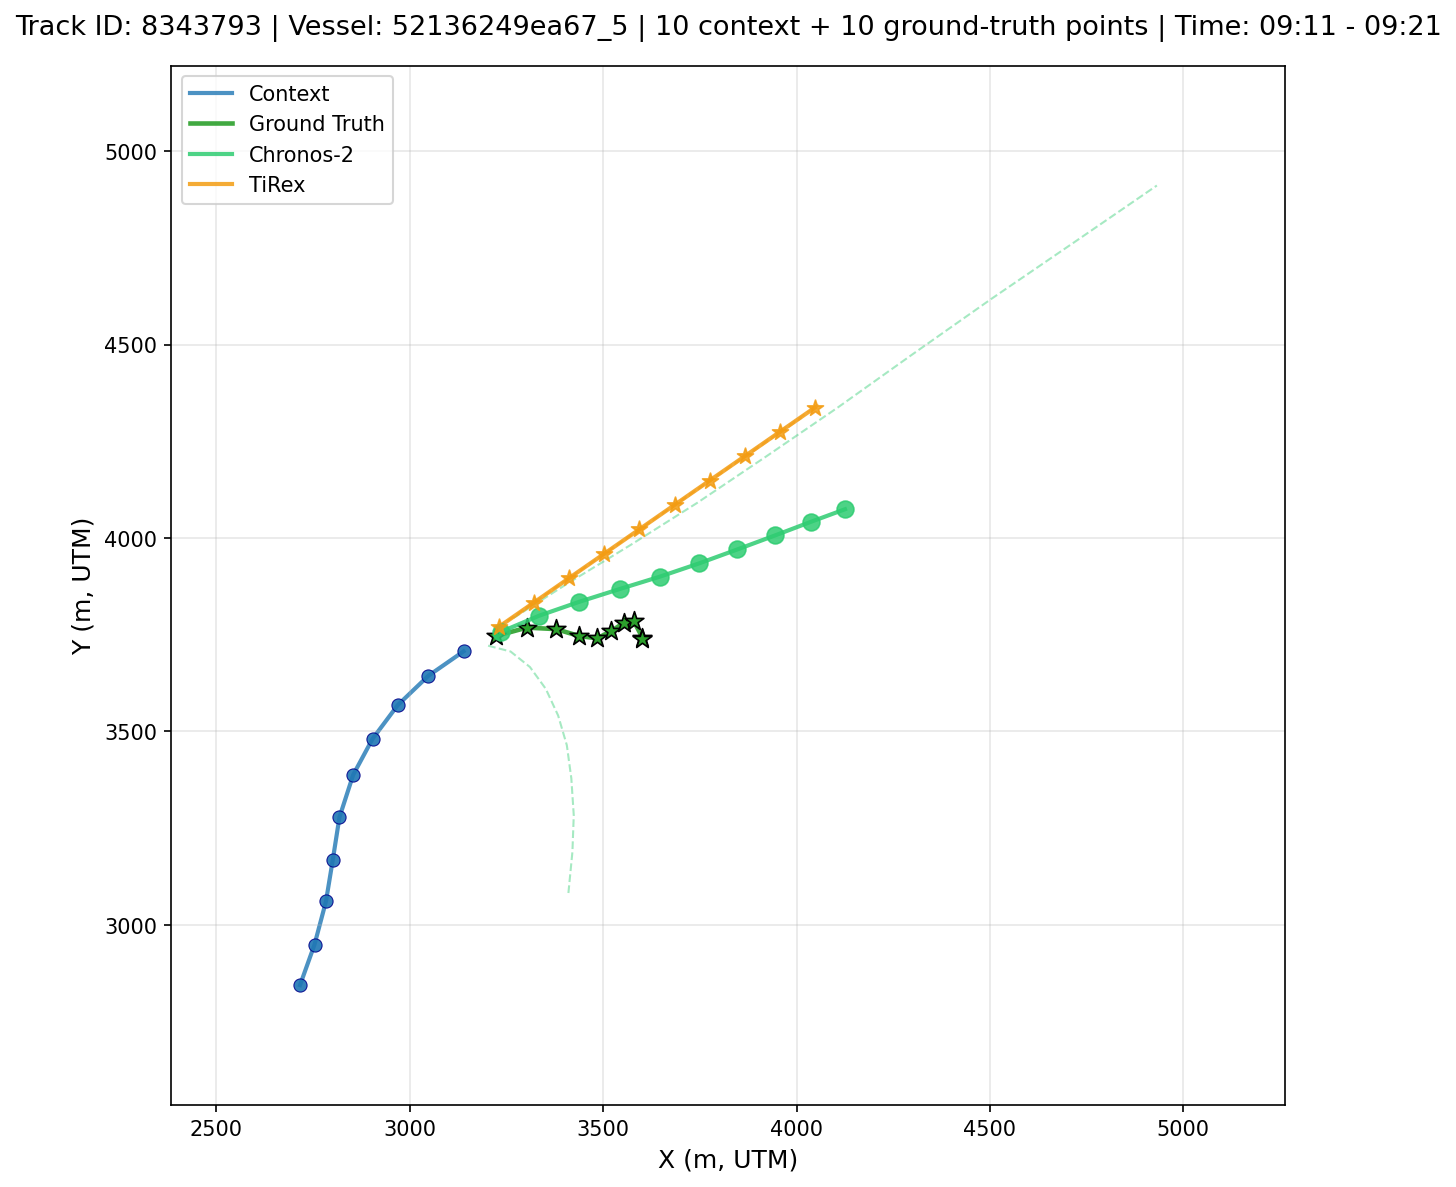
\includegraphics[width=\linewidth, trim=0 0 0cm 1.6cm,clip]{figures/domain23.png}
    \end{subfigure}
    \hfill
    \begin{subfigure}[t]{0.49\textwidth}
        \centering
        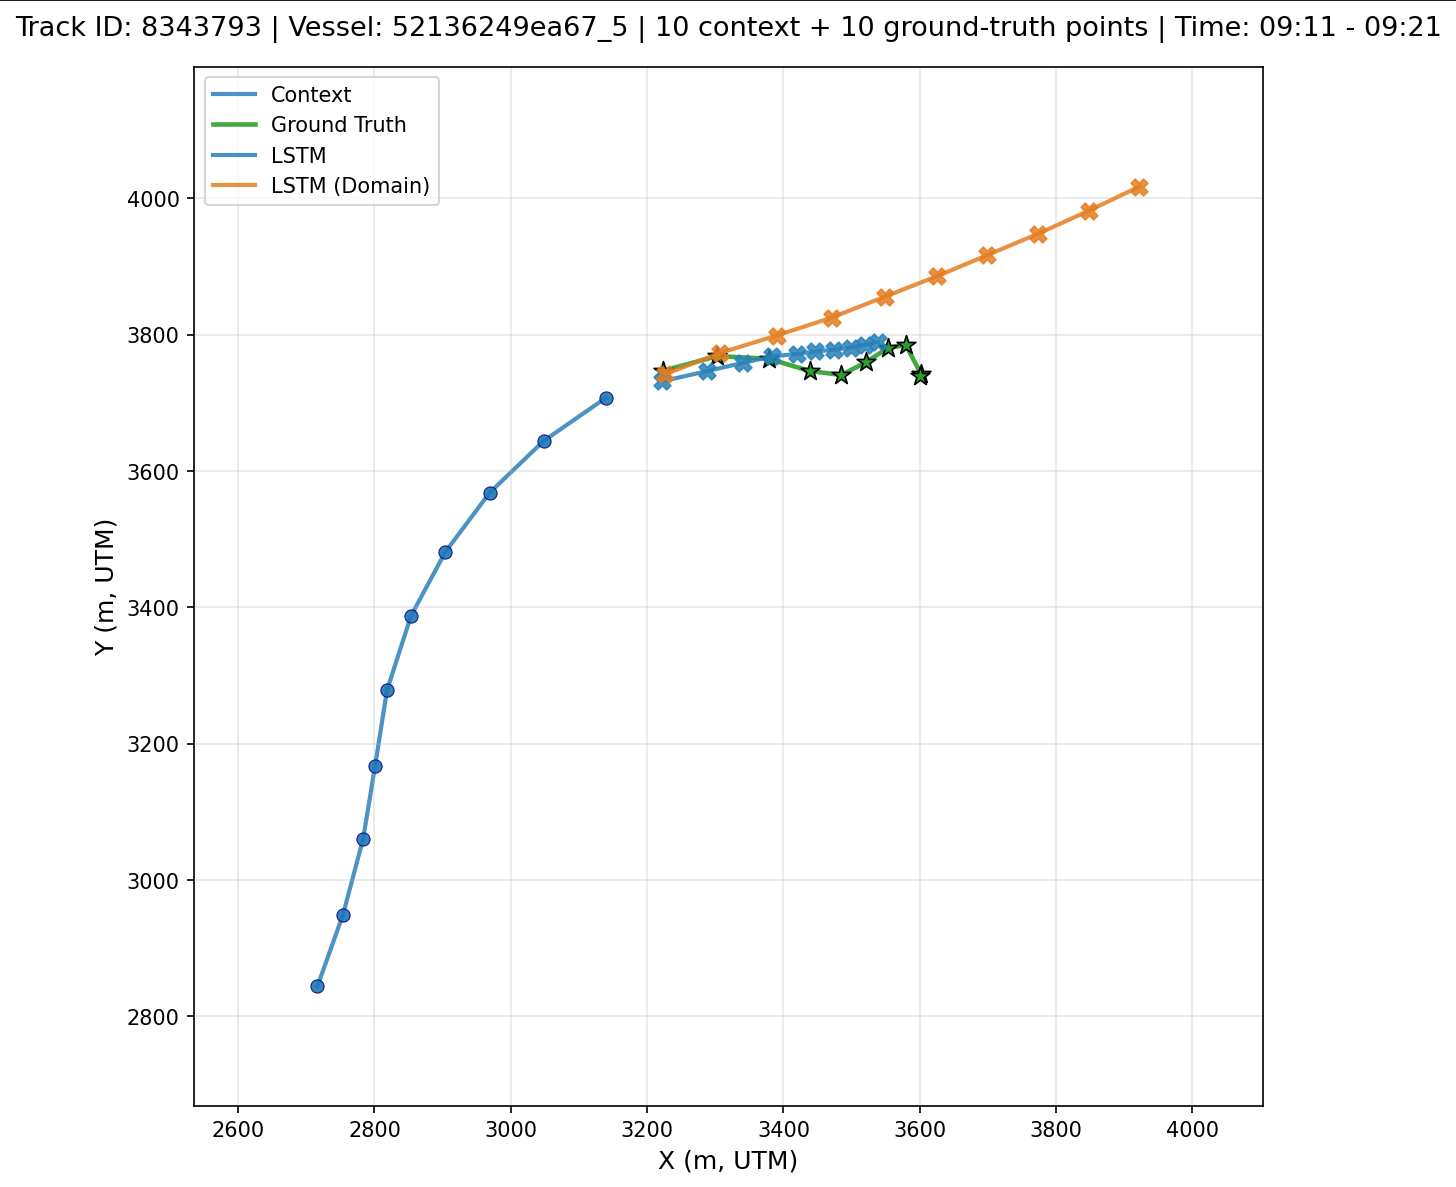
\includegraphics[width=\linewidth, trim=0 0 0cm 1.6cm,clip]{figures/domain24.png}
    \end{subfigure}

    \caption[Forecasting examples for Harbour (Kiel)]{Forecasting examples for the Harbour domain (Kiel). These plots provide a qualitative visual comparison of the predicted paths generated by the evaluated models. The observed context window is displayed in blue, while the actual ground truth trajectory that follows is marked with green stars. The various model predictions are shown in the remaining colours. For Chronos 2, the 80\% certainty band is displayed using thin green dots. Both axes represent relative \ac{UTM} coordinates measured in meters.}    \label{fig:domain2}
\end{figure}

\FloatBarrier
\clearpage

% =========================
% Domain 3
% =========================
\begin{figure}[p]
    \centering

    \begin{subfigure}[t]{0.95\textwidth}
        \centering
        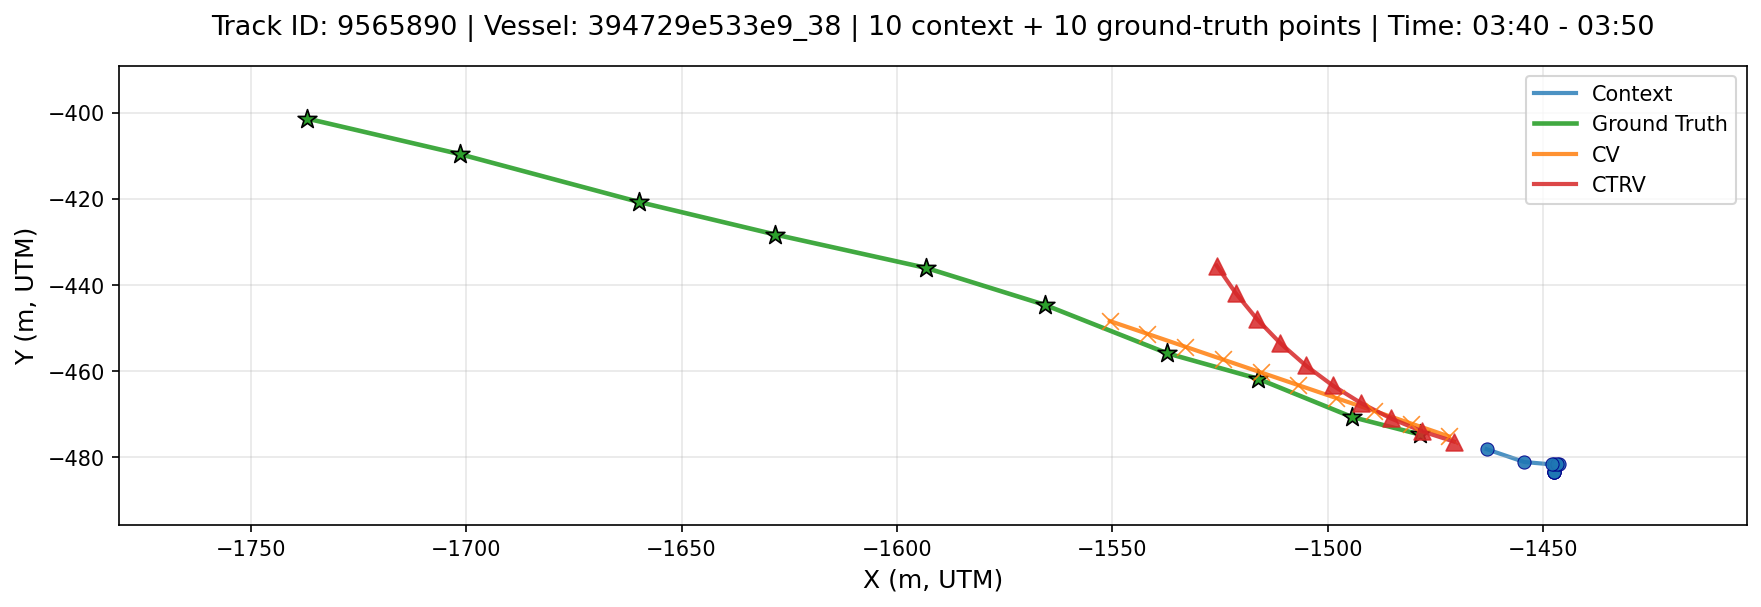
\includegraphics[width=\linewidth, trim=0 0 0cm 1.5cm,clip]{figures/domain31.png}
    \end{subfigure}

    \vspace{0.5em}

    \begin{subfigure}[t]{0.95\textwidth}
        \centering
        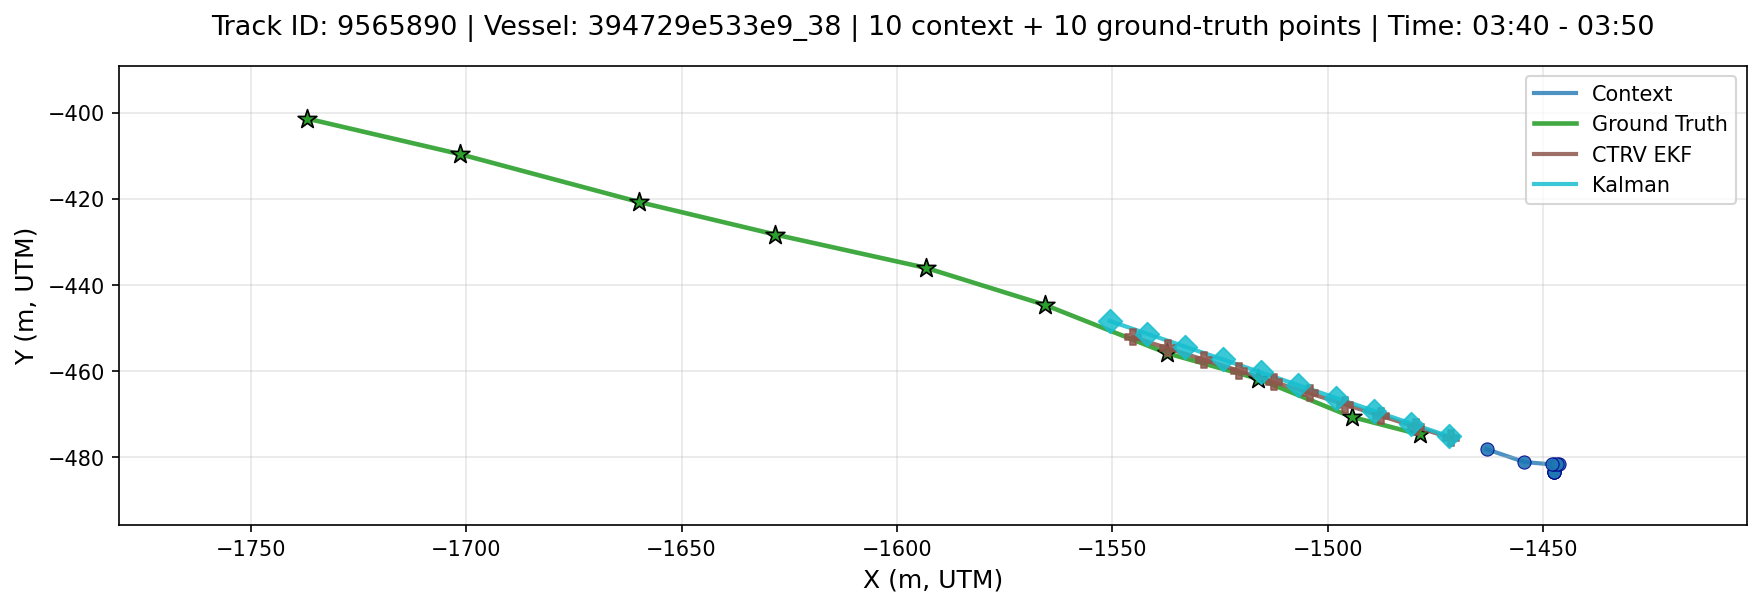
\includegraphics[width=\linewidth, trim=0 0 0cm 1.5cm,clip]{figures/domain32.png}
    \end{subfigure}

    \vspace{0.5em}

    \begin{subfigure}[t]{0.95\textwidth}
        \centering
        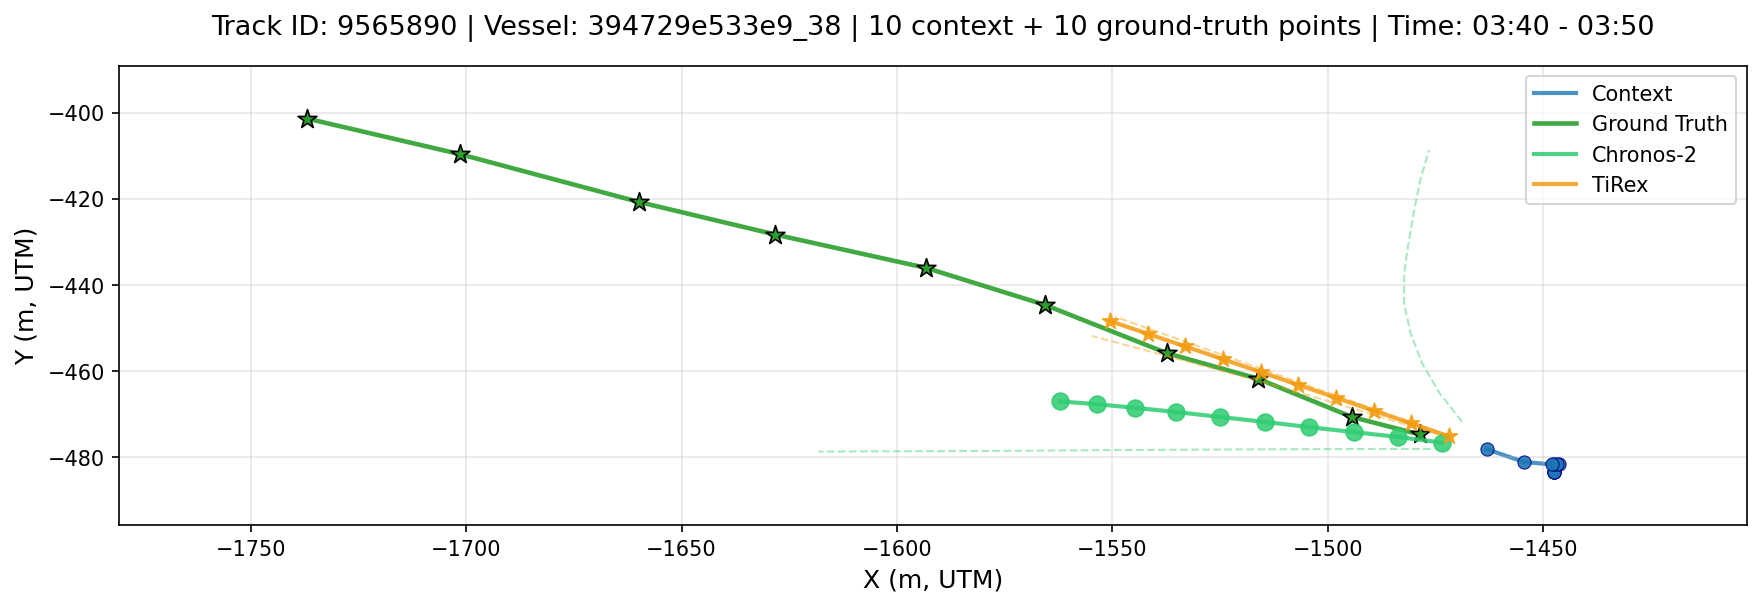
\includegraphics[width=\linewidth, trim=0 0 0cm 1.5cm,clip]{figures/domain33.png}
    \end{subfigure}

    \vspace{0.5em}

    \begin{subfigure}[t]{0.95\textwidth}
        \centering
        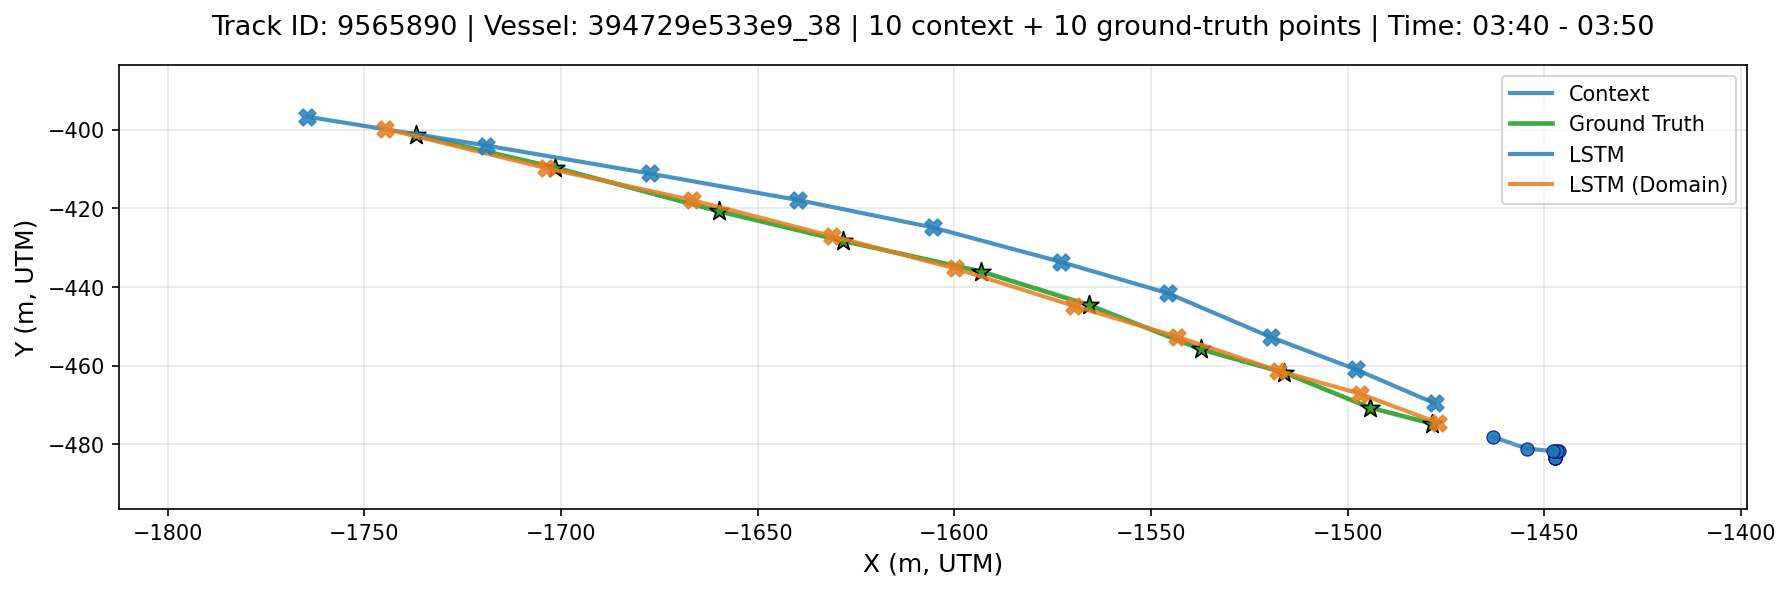
\includegraphics[width=\linewidth, trim=0 0 0cm 1.5cm,clip]{figures/domain34.png}
    \end{subfigure}

    \caption[Forecasting examples for Lock (Kiel)]{Forecasting examples for the Lock domain (Kiel). These plots provide a qualitative visual comparison of the predicted paths generated by the evaluated models. The observed context window is displayed in blue, while the actual ground truth trajectory that follows is marked with green stars. The various model predictions are shown in the remaining colours. For Chronos 2, the 80\% certainty band is displayed using thin green dots. Both axes represent relative \ac{UTM} coordinates measured in meters.}    \label{fig:domain3}
\end{figure}

\FloatBarrier
\clearpage

% =========================
% Domain 4
% =========================
\begin{figure}[p]
    \centering

    \begin{subfigure}[t]{0.95\textwidth}
        \centering
        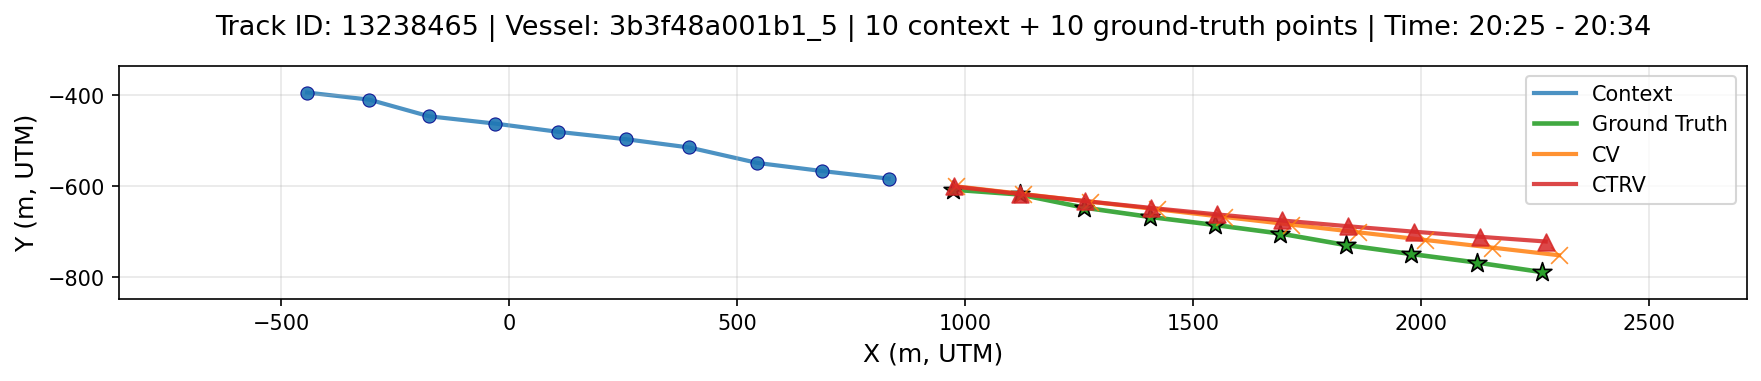
\includegraphics[width=\linewidth, trim=0 0 0cm 1.5cm,clip]{figures/domain41.png}
    \end{subfigure}

    \vspace{0.5em}

    \begin{subfigure}[t]{0.95\textwidth}
        \centering
        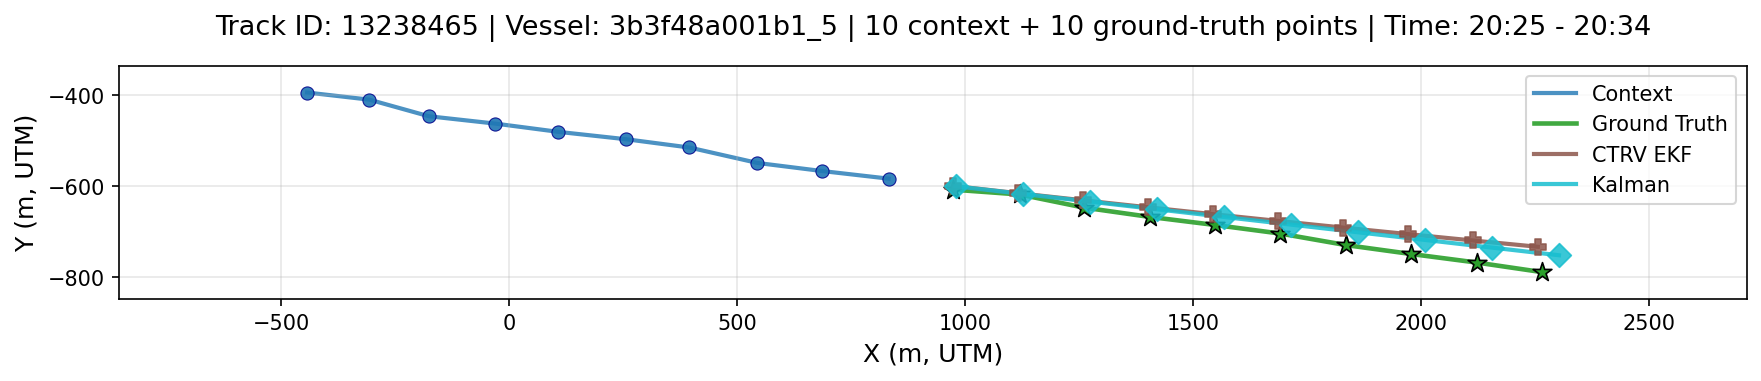
\includegraphics[width=\linewidth, trim=0 0 0cm 1.5cm,clip]{figures/domain42.png}
    \end{subfigure}

    \vspace{0.5em}

    \begin{subfigure}[t]{0.95\textwidth}
        \centering
        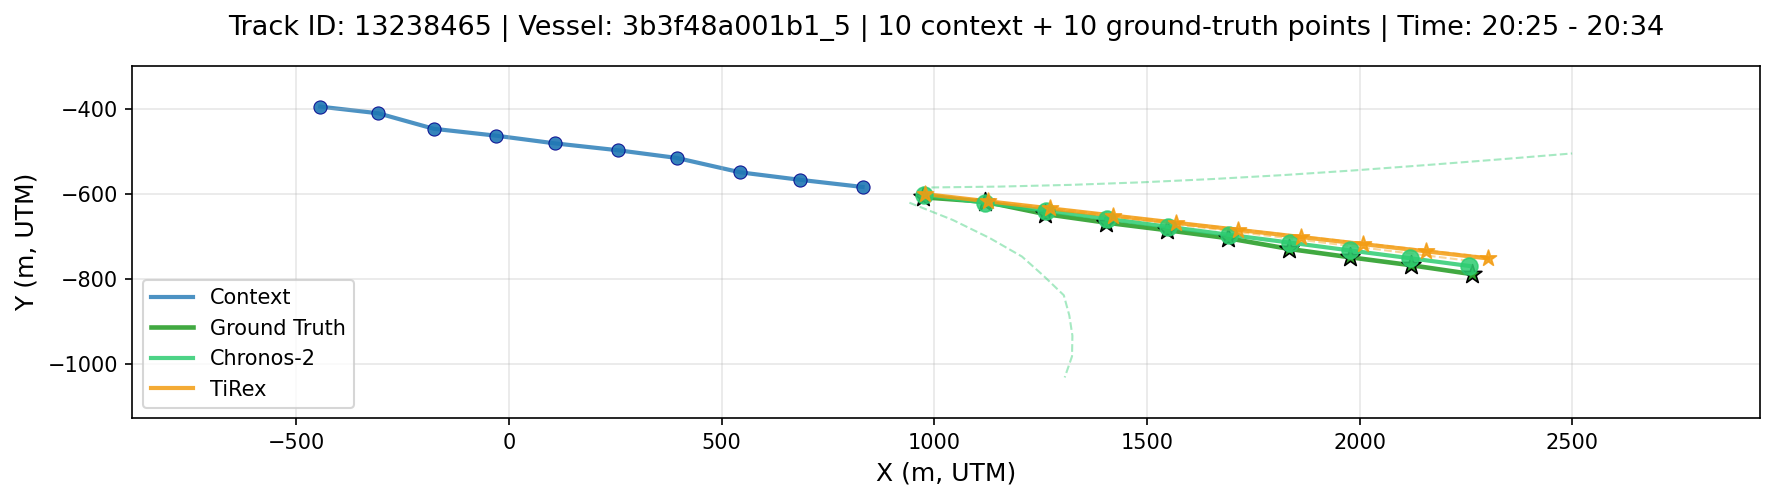
\includegraphics[width=\linewidth, trim=0 0 0cm 1.5cm,clip]{figures/domain43.png}
    \end{subfigure}

    \vspace{0.5em}

    \begin{subfigure}[t]{0.95\textwidth}
        \centering
        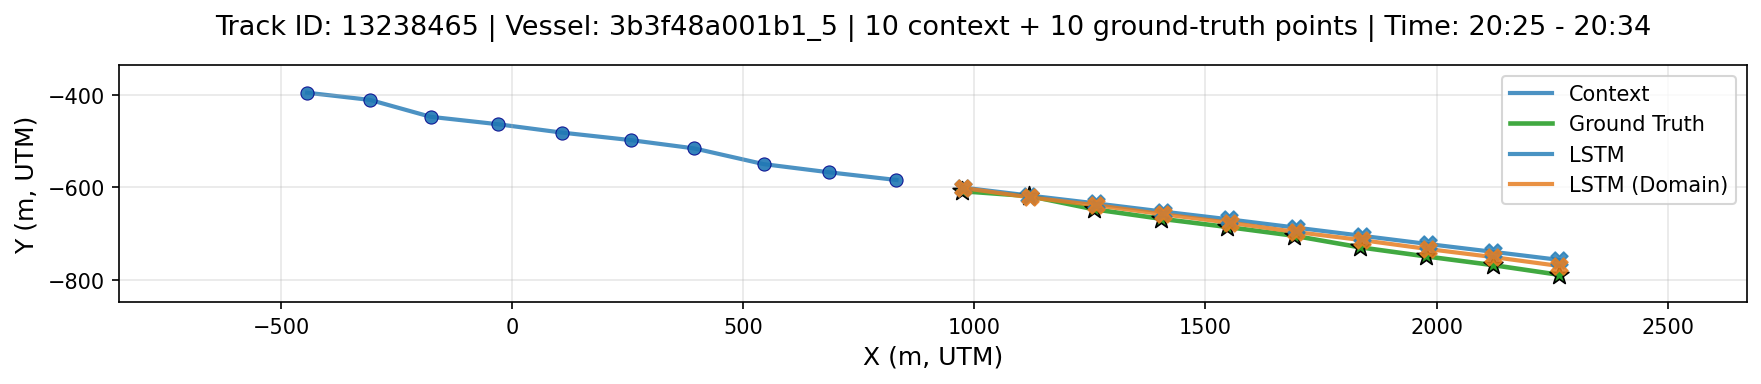
\includegraphics[width=\linewidth, trim=0 0 0cm 1.5cm,clip]{figures/domain44.png}
    \end{subfigure}

    \caption[Forecasting examples for River (Wedel)]{Forecasting examples for the River domain (Wedel). These plots provide a qualitative visual comparison of the predicted paths generated by the evaluated models. The observed context window is displayed in blue, while the actual ground truth trajectory that follows is marked with green stars. The various model predictions are shown in the remaining colours. For Chronos 2, the 80\% certainty band is displayed using thin green dots. Both axes represent relative \ac{UTM} coordinates measured in meters.}    \label{fig:domain4}
\end{figure}








% Seite 1: CD Diagrams 1–2
\begin{figure}[p]
    \centering
    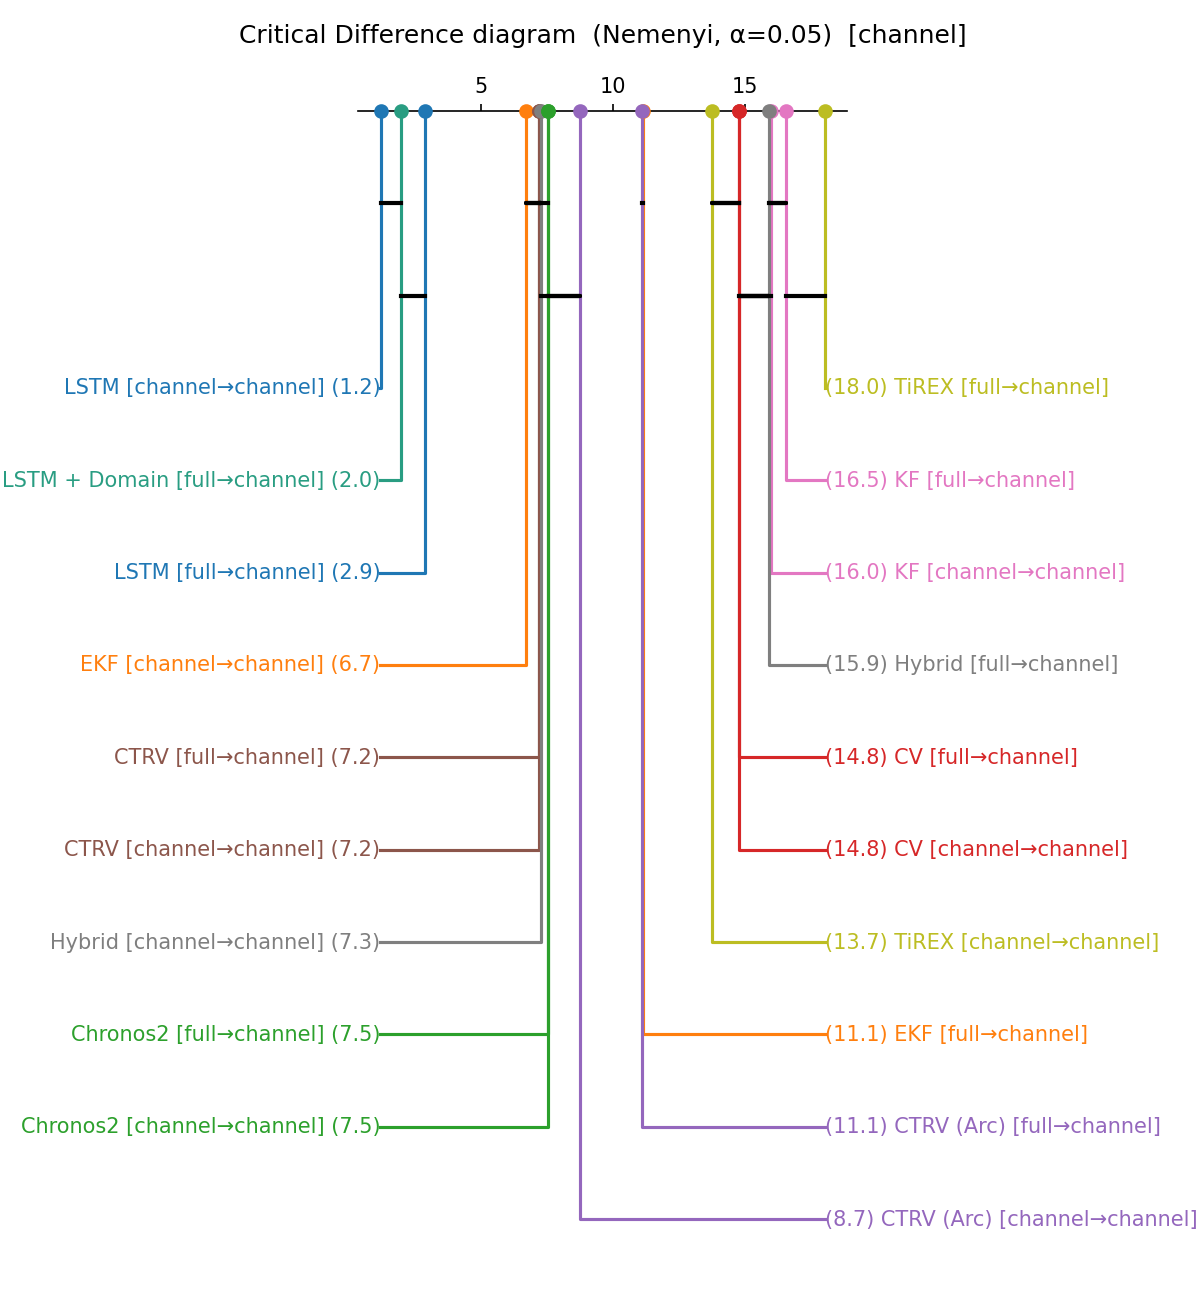
\includegraphics[height=0.48\textheight]{figures/cd_diagram_channel}\\[4pt]
    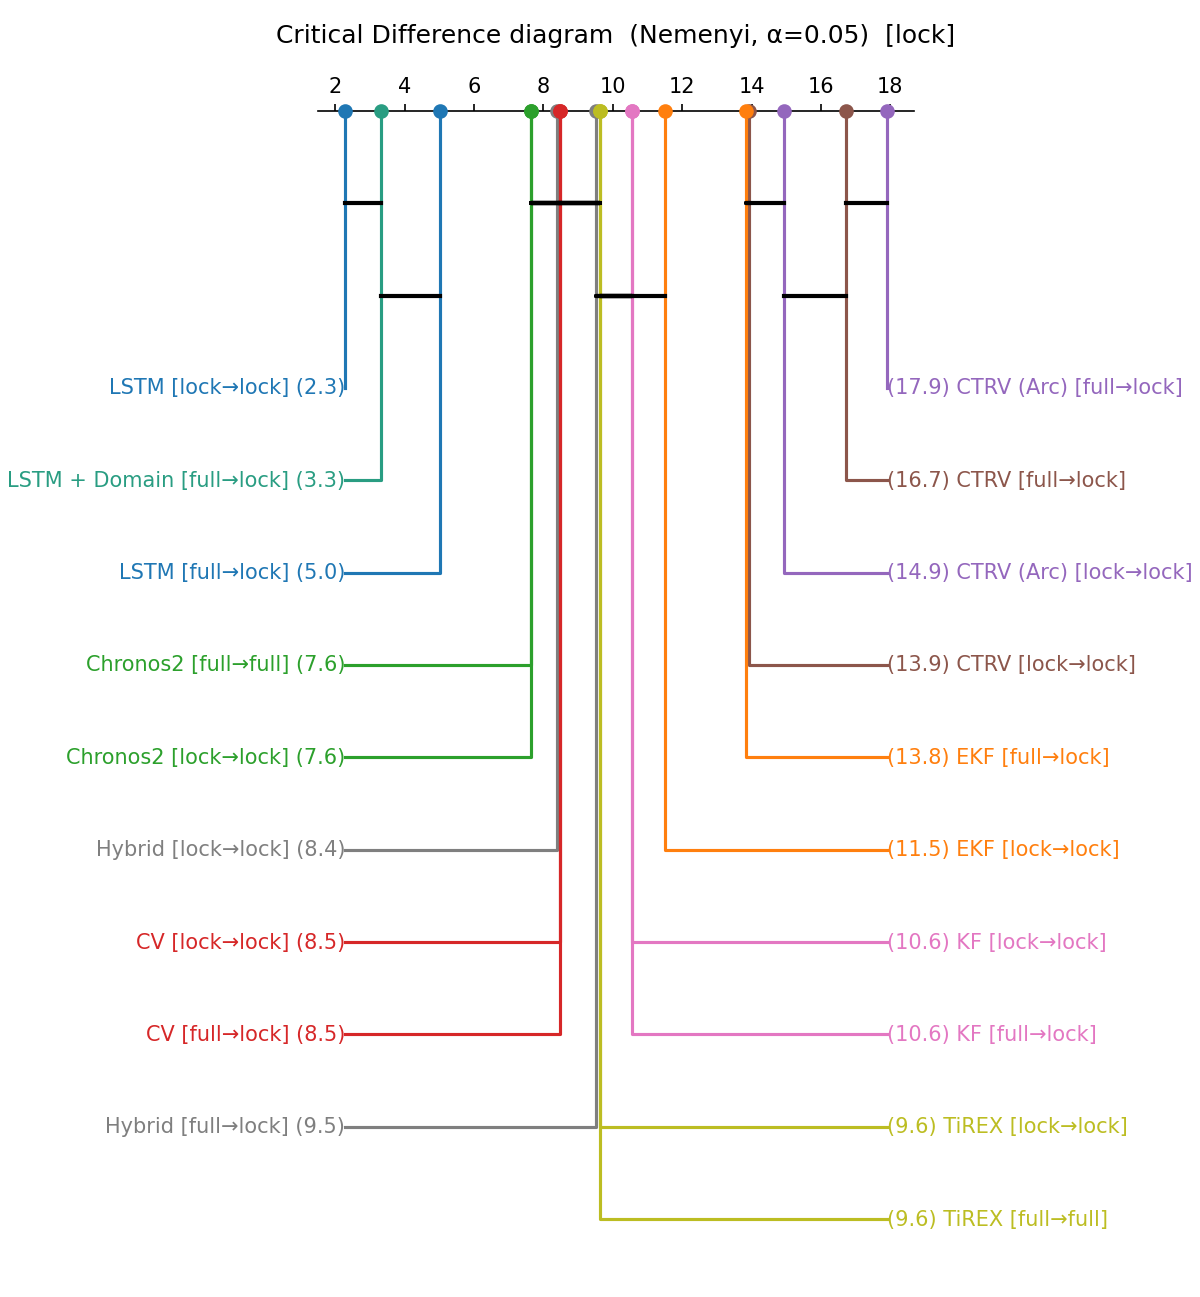
\includegraphics[height=0.48\textheight]{figures/cd_diagram_lock}
    \caption[Exp. II Friedman \& Nemenyi CD-Plots (1/2)]{\acf{CD} diagram based on the Friedman test and Nemenyi post-hoc comparison for mixed and domain specific training, evaluated per domain. Models connected by a horizontal bar are not significantly different at \( \alpha = 0.05\). The shown numbers are the mean rank per model in the evaluation, 1 being the best possible result. It can be observed that the harbour domain is the only environment where domain-specific training fails to produce a statistically significant improvement for the \ac{LSTM} (1/2).}
    \label{fig:cd-diagrams-a}
\end{figure}

% Seite 2: CD Diagrams 3–4
\begin{figure}[p]
    \ContinuedFloat
    \centering
    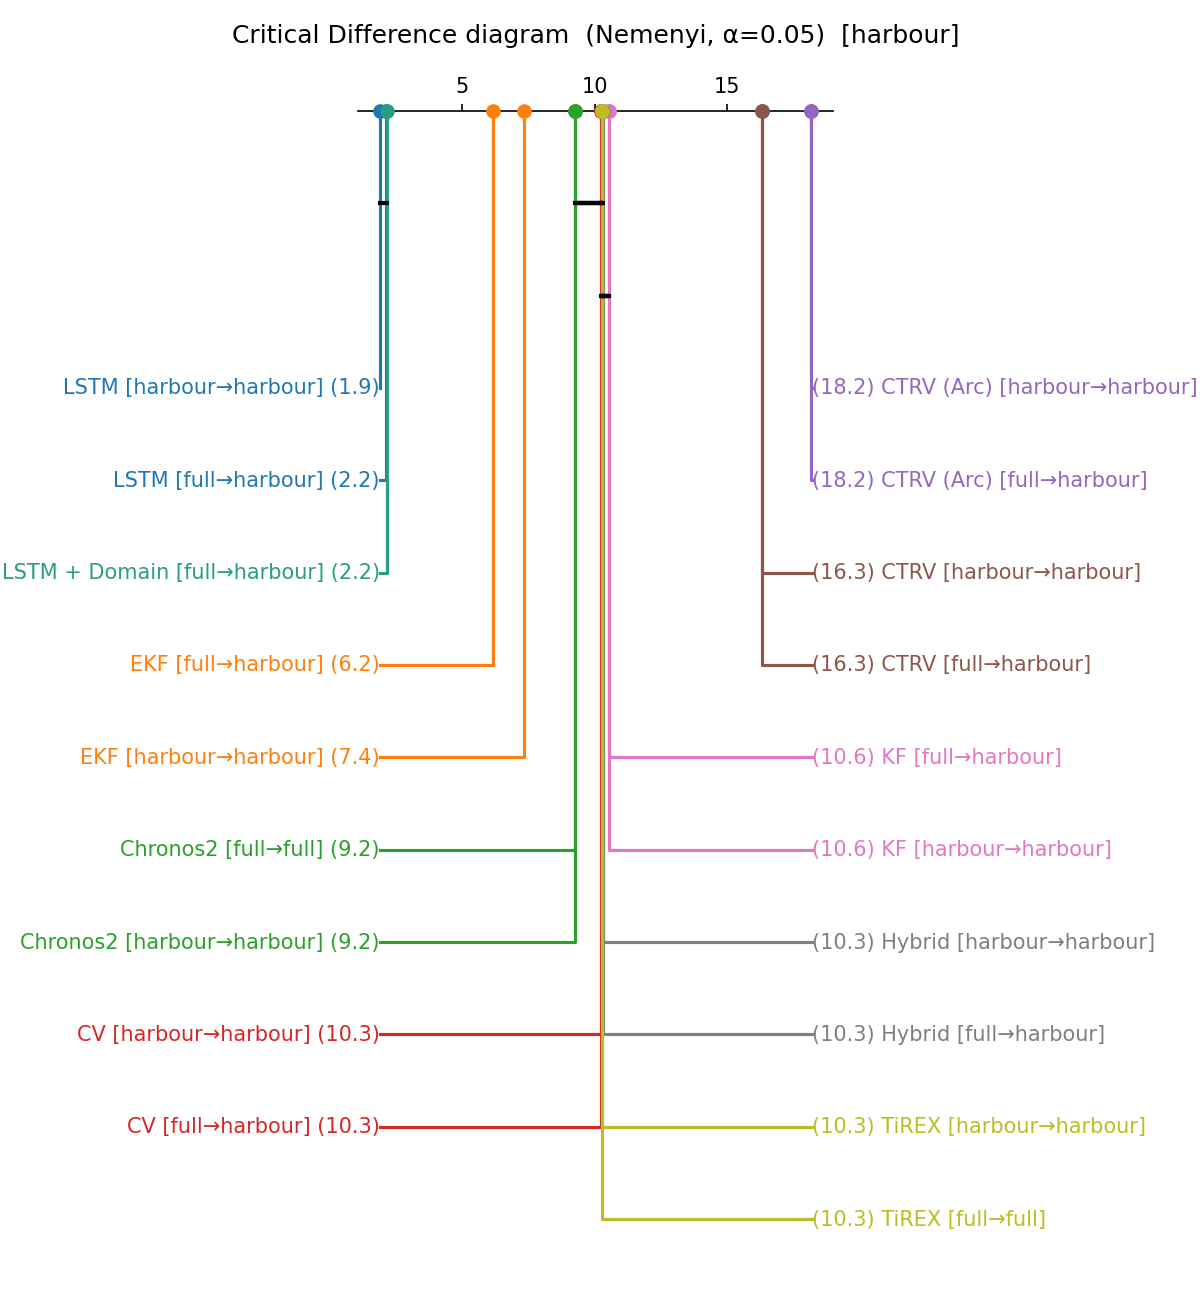
\includegraphics[height=0.48\textheight]{figures/cd_diagram_harbour}\\[4pt]
    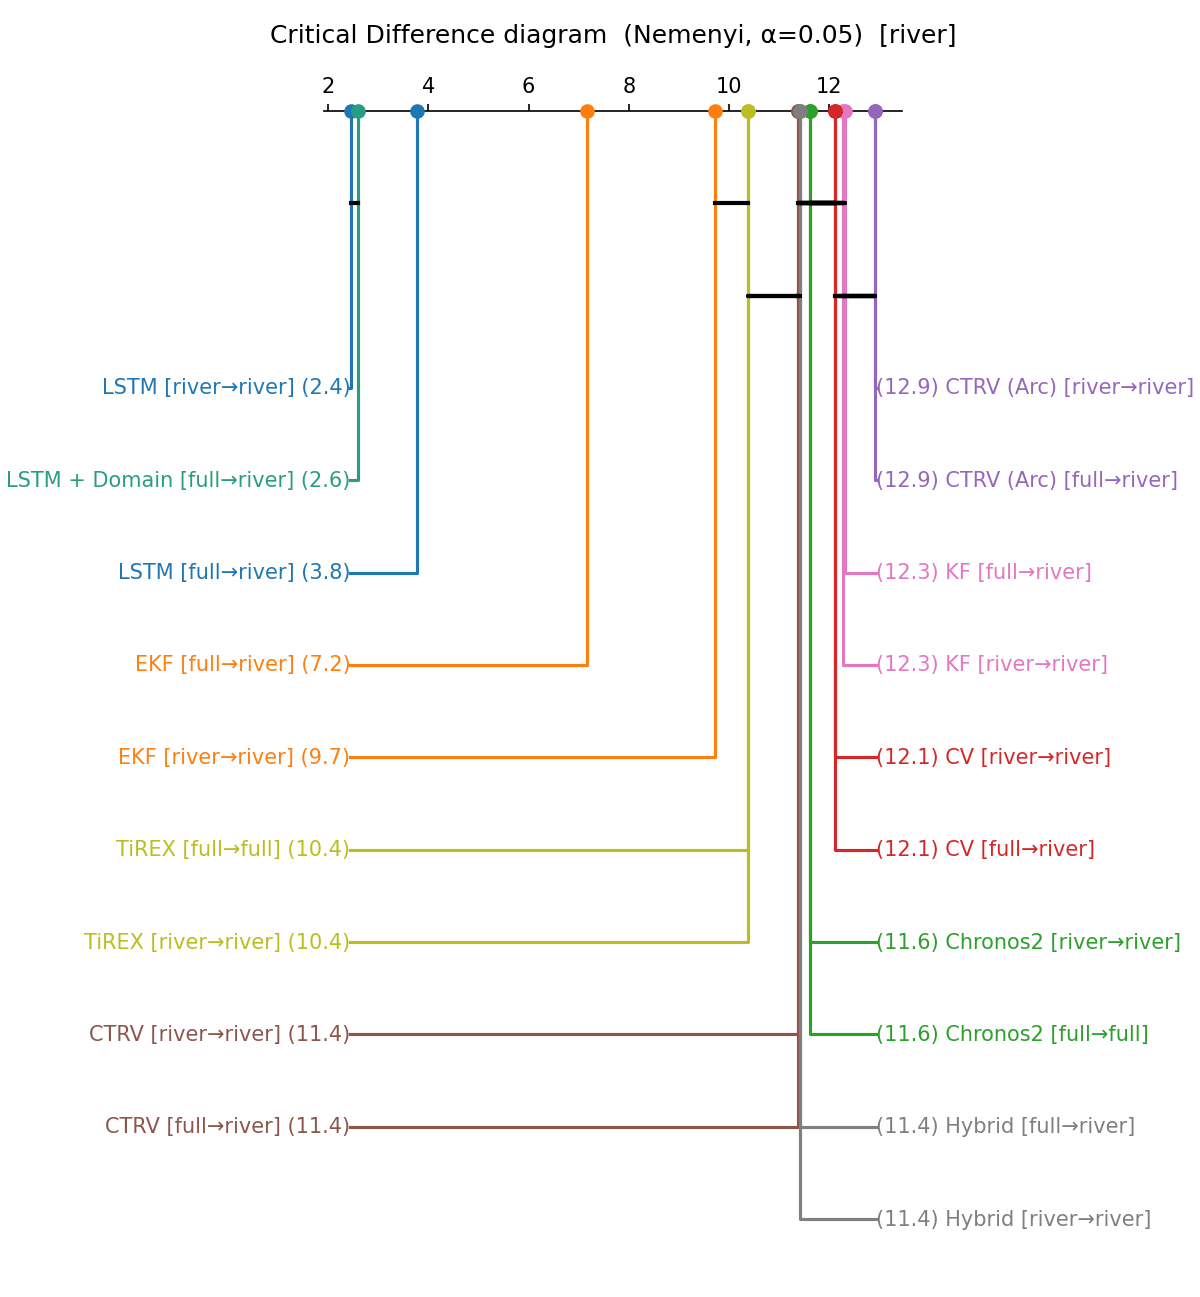
\includegraphics[height=0.48\textheight]{figures/cd_diagram_river}
    \caption[Exp. II Friedman \& Nemenyi CD-Plots (2/2)]{\acf{CD} diagram based on the Friedman test and Nemenyi post-hoc comparison for mixed and domain specific training, evaluated per domain. Models connected by a horizontal bar are not significantly different at \( \alpha = 0.05\). The shown numbers are the mean rank per model in the evaluation, 1 being the best possible result. It can be observed that the harbour domain is the only environment where domain-specific training fails to produce a statistically significant improvement for the \ac{LSTM} (2/2).}
    \label{fig:cd-diagrams-b}
\end{figure}

\begin{comment}
adjust caption if put in appendix again
    \begin{figure}
    \centering
    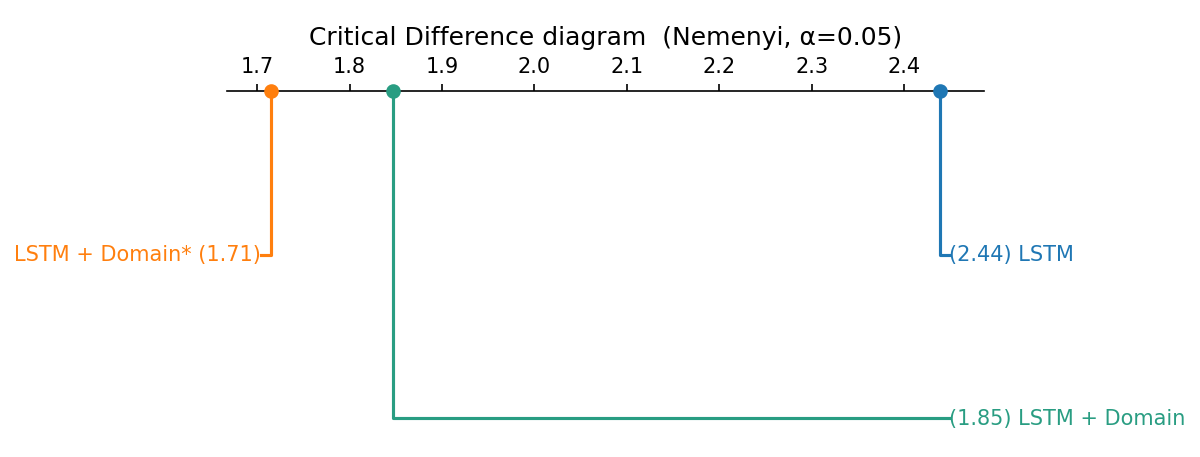
\includegraphics[width=0.75\linewidth]{figures/cd_diagram_lstm_comparison.png}
    \caption{Critical Difference Diagrams for LSTM domain encoding (mixed training and evaluation)}
    \label{fig:cd_exp3}
\end{figure}

\end{comment}






\FloatBarrier
\clearpage

\FloatBarrier

\chapter{Supplementary Tables} %unpassend
\label{appx:B}





\begin{table}[t]%%%%%%%%%%%% OPTIMiseR
    \centering
    %\caption{HPO Optimiser Configurations}
    \caption[Configuration Parameters for Optuna HPO]{Configuration parameters for the Optuna hyperparameter optimisation. The table details the specific search algorithms, trial counts, seeding strategies, and early stopping criteria applied to each model type, ranging from kinematic models to the LSTM.}
    \label{tab:hpo-config}
    \scalebox{1}{%  %% 5% smaller (0.95 = 95% of original size)

    \setlength{\tabcolsep}{4pt}  %% Reduce from default 6pt

    \begin{tabular}{ll}
        \toprule
        \textbf{Parameter} & \textbf{Value} \\
        \midrule
        \multicolumn{2}{l}{\textit{General}} \\
        HPO Framework       & Optuna \\ %\makecell[l]{Optuna (Grid Search for 1D HPO,\\TPE Sampler otherwise)} \\
        Device & CUDA (2 x RTX 4090) \\
        TPE Multivariate    & false \\
        Early Stopping Patience & 50 trials \\
        Early Stopping Min.\ Delta & $10^{-4}$ \\
        Random Seed & 42 \\

        \midrule
        \multicolumn{2}{l}{\textit{CV / CTRV / CTRV Arc}} \\
        Method              & Grid Search (1D) \\
        Search Space        & $ [1,\ \text{max}]$ \\
        \midrule
        \multicolumn{2}{l}{\textit{Hybrid CV/CTRV}} \\
        Method              & TPE \\
        Number of Trials    & 100 \\
        TPE Startup Trials  & 20 \\
        Seeded Initial Trial & CV/CTRV best \texttt{velocity\_steps} \\
        \midrule
        \multicolumn{2}{l}{\textit{Kalman Filter \& EKF}} \\
        Method              & TPE \\
        Number of Trials    & 100 \\
        TPE Startup Trials  & 20 \\
     
        \midrule
        \multicolumn{2}{l}{\textit{LSTM}} \\
        Method              & TPE + Successive Halving Pruner \\
        Number of Trials    & 100 \\
        TPE Startup Trials  & 26 (16 feature sets $+$ 10) \\
        Seeded Initial Trials & 16 (one per feature set) \\
        Pruner Min.\ Resource & 8 epochs \\
        Pruner Reduction Factor & 2 \\
        Pruner Min.\ Early Stopping Rate & 0 \\
        Max.\ Epochs        & 100 \\
        Training Patience   & 8 epochs \\
        Training Min.\ Delta & $10^{-4}$ \\
        \bottomrule
        \vspace{-2pt}
    \end{tabular}
    }%scalebox
\end{table}









    \begin{table}[t] %%%%%%---------- HP list - todo move to appendix if no space 
    \centering
    \caption[Model-specific Hyperparameters]{Model-specific hyperparameters used in the experiments.}
    \label{tab:model_hyperparameters}
    \begin{tabular}{ll}
    \toprule
    \textbf{Model} & \textbf{Hyperparameters} \\
    \midrule
    CV & $n_\text{vel}$ \\
    CTRV & $n_\text{vel}$ \\
    CTRV Arc & $n_\text{vel}$ \\
    Hybrid CV/CTRV & $n_\text{vel}^\text{CV}$, $n_\text{vel}^\text{CTRV}$, $n_\text{rot}$, $\tau_\text{rot}$ \\
    KF (CV) & $q_\text{pos}$, $q_\text{vel}$, $r_\text{pos}$, $p_{0,\text{pos}}$, $p_{0,\text{vel}}$ \\
    EKF (CTRV) & $q_\text{pos}$, $q_\text{vel}$, $q_\text{rot}$, $r_\text{pos}$, $p_{0,\text{pos}}$, $p_{0,\text{vel}}$, $p_{0,\text{rot}}$, $n_\text{ctx}$ \\
    Chronos-2 & -- \\
    TiREX & context length \\
    LSTM & hidden size, number of layers, dropout, learning rate, batch size, feature set \\
    LSTM + Domain & hidden size, number of layers, dropout, learning rate, batch size, feature set \\
    \bottomrule
    \end{tabular}
    \end{table} 





















%**************************************

\chapter{Methodological Details} 
\label{chap:appendixderivations}

\section{Mathematical Foundations of Sequence Models}
\label{appx: mathfoundations}
In this appendix, we present more details on the mathematical formalisations underlying the sequence models discussed in the main text.
\subsection*{\acf{RNN}}
Building on the first popular model to use recurrence, the Hopfield Network introduced by \textcite{hopfieldrnn}, the foundational concept for sequence-based learning is the \ac{RNN}. 
The primary distinction between \acp{RNN} and conventional Feedforward Neural Networks, such as \acp{MLP}, is the direction of information flow. 
While the latter are acyclic, \acp{RNN} use cycles to feed information back into the hidden state. 
With this architecture, the model incorporates context from previous inputs $X_{0:t-1}$ when processing the current input $X_t$, instead of processing each input in isolation \parencite{gentleschmidt2019recurrentneuralnetworksrnns}.
The basic structure of this recurrent process, configured as an Encoder-Decoder architecture, is illustrated in Figure~\ref{fig:s2s_rnn_appendix}.
Consequently, the network can make decisions based on the patterns it recognises \parencite{AIBook}. 
The recurrence can be expressed as Equation \ref{eq:app1},
\begin{equation}
    H_t = \phi_h (X_t W_{xh} + H_{t-1} W_{hh} + b_h) 
    \label{eq:app1}
\end{equation}
where $W$ represents weight matrices and $\phi$ an activation function. 
Despite their theoretical capability to handle sequences, \acp{RNN} suffer from the \emph{vanishing gradient problem}, as well as the \emph{exploding gradient problem}, as established by \textcite{279181bengio}.
As the sequence length increases, the gradients used to update weights during backpropagation decrease exponentially. 
This exponential decrease prevents the model from learning long-term dependencies.

\subsection*{\acf{LSTM}}
To address the limitations of standard \acp{RNN} to capture long-term dependencies, \textcite{hochreiterLSTM} introduced the \ac{LSTM} architecture. 
The corresponding archtiecture of the \ac{LSTM}-based Encoder-Decoder model is depicted in Figure~\ref{fig:s2s_lstm_appendix}.
The core innovation of the \ac{LSTM} is the introduction of a cell state $C_t$. 
Through this state, information persists across many time steps. 
The flow of information in and out of these cells is regulated by three gates:
\begin{itemize}
    \item \textbf{Forget Gate $F_t$}: Determines which information from the previous cell state $C_{t-1}$ is no longer needed and should be discarded.
    \item \textbf{Input Gate $I_t$}: Decides which new information from the current input $X_t$ and previous hidden state $H_{t-1}$ is relevant to be stored in the cell state.
    \item \textbf{Output Gate $O_t$}: Controls which parts of the current cell state $C_t$ are used to compute the new hidden state $H_t$.
\end{itemize}

Following the formalisation by \textcite{gentleschmidt2019recurrentneuralnetworksrnns}, the internal update process can be defined by Equation~\ref{eq:lstm_updates}:
\begin{equation}
    \begin{aligned}
        F_t &= \sigma(X_t W_{xf} + H_{t-1} W_{hf} + b_f), \\
        I_t &= \sigma(X_t W_{xi} + H_{t-1} W_{hi} + b_i), \\
        \tilde{C}_t &= \tanh(X_t W_{xc} + H_{t-1} W_{hc} + b_c), \\
        C_t &= F_t \odot C_{t-1} + I_t \odot \tilde{C}_t, \\
        O_t &= \sigma(X_t W_{xo} + H_{t-1} W_{ho} + b_o), \\
        H_t &= O_t \odot \tanh(C_t).
    \end{aligned}
    \label{eq:lstm_updates}
\end{equation}

In these equations, $\tilde{C}_t$ represents a candidate cell state, $\sigma$ is the sigmoid activation function $\sigma(x) = \frac{1}{1 + e^{-x}}$, and $\odot$ denotes the element-wise (Hadamard) product.
$W$ and $b$ are the respective weights and biases.
This update procedure for the cell state $C_t$ prevents the gradient from vanishing as quickly as in standard \acp{RNN}.

As indicated by the multi-dimensional input vector $X_t$ and the associated weight matrices, the \ac{LSTM} architecture is mathematically equipped for multivariate sequence modelling. 
The model has the capacity to represent nonlinear cross-channel correlations, because the internal gating mechanisms integrate information from all input features simultaneously.
This integration models their interdependencies within a shared hidden representation.
Consequently, this design is highly suitable for the present use case.

\begin{figure}[htbp]
    \centering
    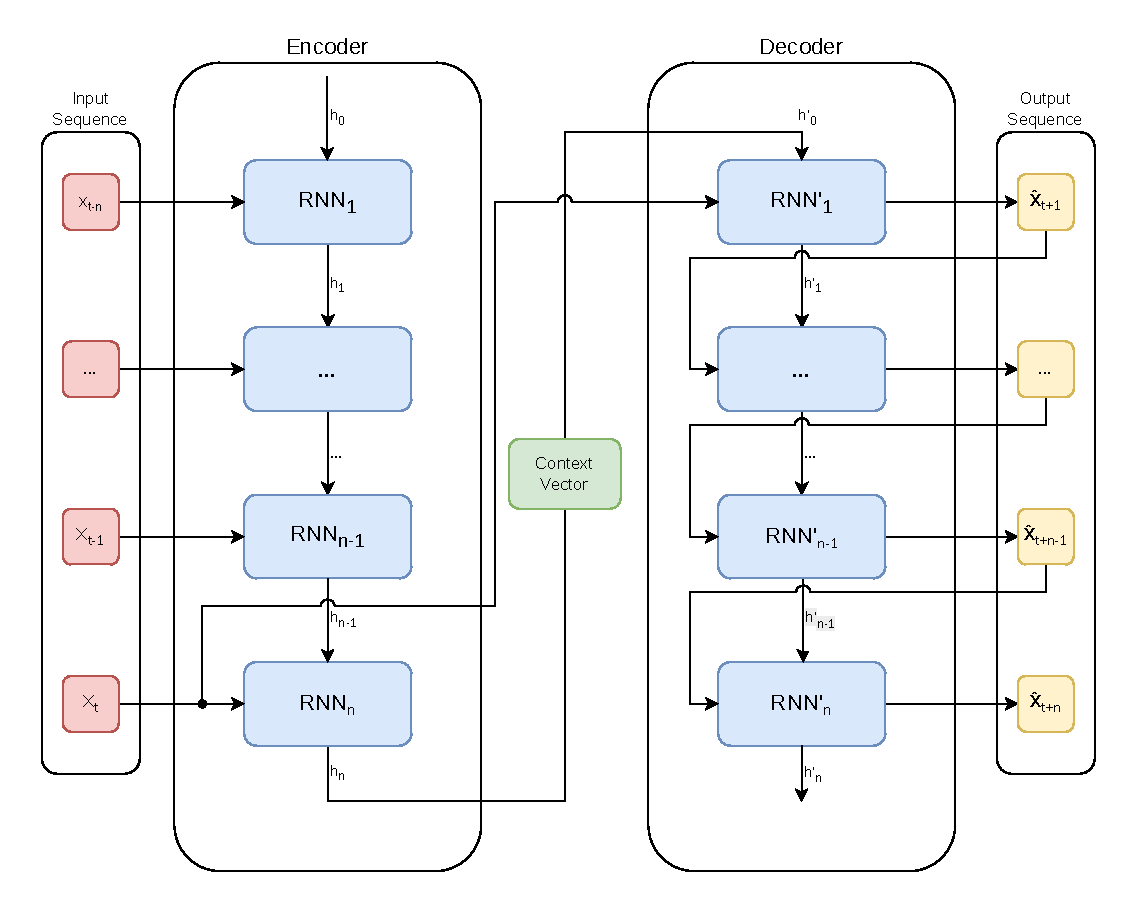
\includegraphics[width=0.75\linewidth]{figures/S2S_RNN.drawio (1).pdf}
    \caption[RNN Architecture]{Architecture of the standard \acf{RNN} Encoder-Decoder model (1 Layer).}
    \label{fig:s2s_rnn_appendix}
\end{figure}

\begin{figure}[htbp]
    \centering
    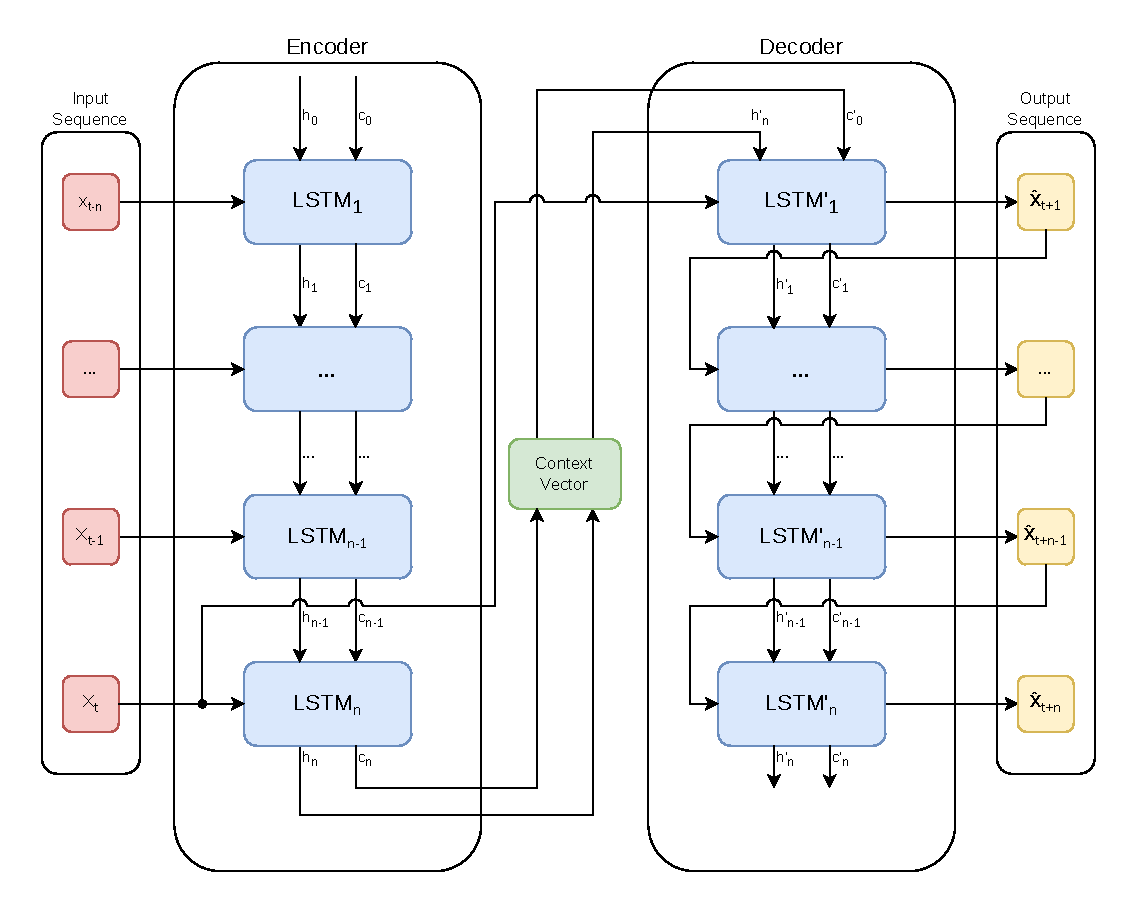
\includegraphics[width=0.75\linewidth]{figures/S2S_LSTM.drawio (1).pdf}
    \caption[LSTM Architecture]{Architecture of the \acf{LSTM} Encoder-Decoder model (1 Layer).}
    \label{fig:s2s_lstm_appendix}
\end{figure}

\newpage % bled into the middle of BO TPE text

\section{Bayesian Optimisation and the Tree-Parzen-Estimator}
\label{appx:BOandTPE}



In \acf{BO}, past evaluations are used to make informed decisions about which hyperparameters to test next.
This approach is critical for models where evaluating the true objective function $\mathcal{L}$ is computationally expensive (e.g., when fully training an \ac{LSTM}) \parencite{hutter2019automated}.
In \ac{BO}, this is achieved by constructing a probabilistic surrogate model $\hat{f}$, which approximates the true, expensive loss function based on all previously evaluated configurations.
Because the surrogate model $\hat{f}$ is computationally cheap to evaluate, more potential configurations can be tested to identify the most promising candidates before resources are committed to a full model training.

To decide which configuration to evaluate next based on the given surrogate model, an acquisition function is utilised.
A commonly applied acquisition function is \acf{EI} \parencite{AutoMLHoos}.
In \ac{EI}, a candidate is evaluated by combining two essential terms: the expected value of the function at a given point, and the associated variance.
This combination provides a trade-off between two competing goals:

\begin{itemize}
    \item \textbf{Exploitation:} By considering the expected value, the search is focused on promising regions of the search space that contain good candidate solutions with high probability.
    \item \textbf{Exploration:} In contrast, the variance term encourages the exploration of unknown areas that are weakly explored, or where candidate solutions of highly variable quality have been observed \parencite{Jones1998}.
\end{itemize}
Figure~\ref{fig:bo_illustration} illustrates one iteration of this process. %published as open acces. Open access works published by Springer Nature are published under Creative Commons licences.tdoo resolved (check licensing, otherwise use the one from the literature overview automl timeseries)

\begin{figure} [h]
    \centering
    % Adjust trim values (left bottom right top) 
    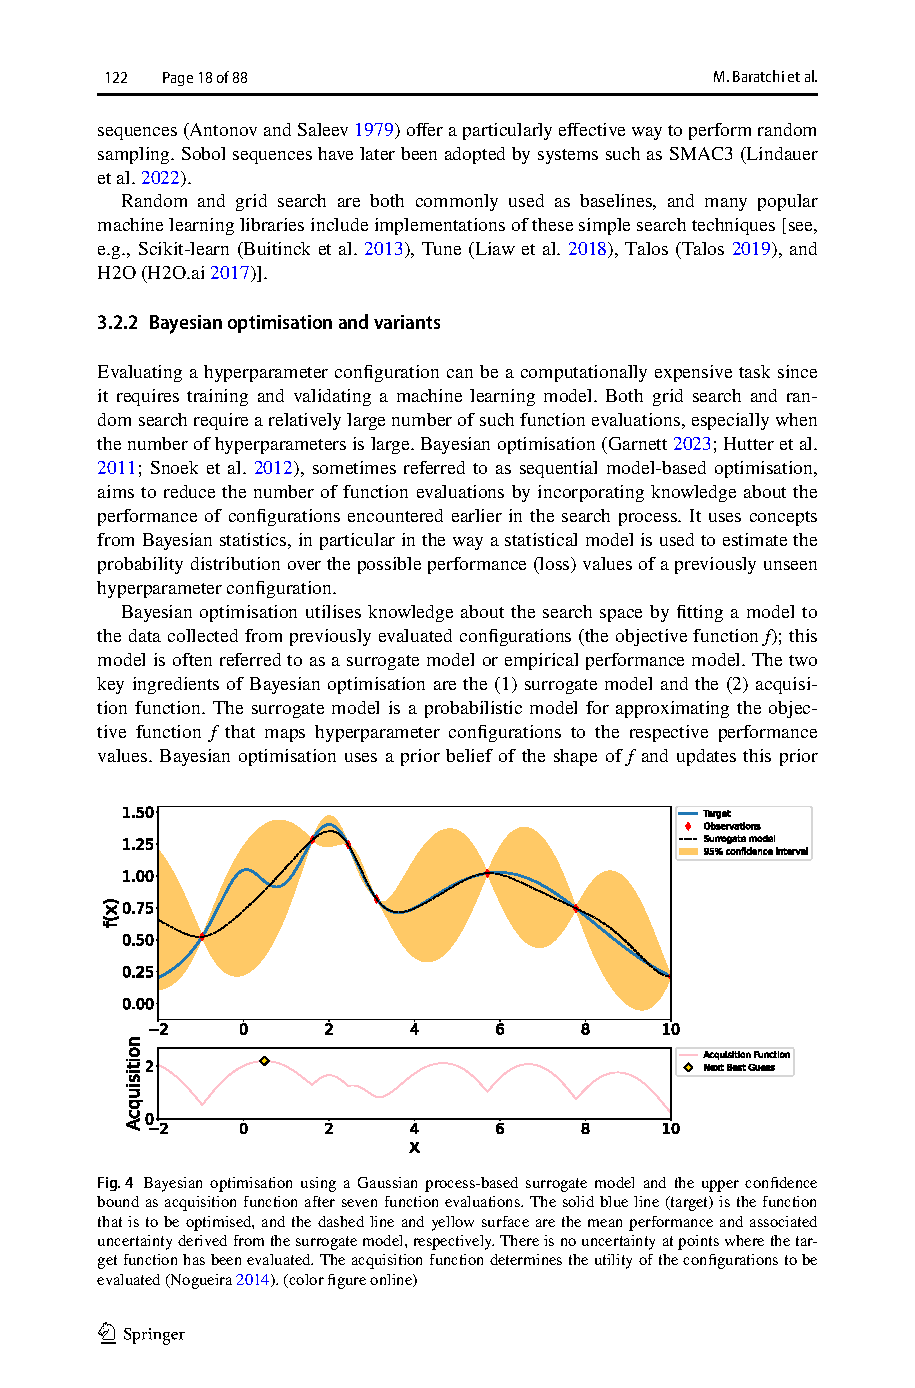
\includegraphics[width=0.9\linewidth,trim={2cm 4cm 2cm 13.5cm}, clip]{figures/985693BO.pdf}
    \caption[Bayesian Optimisation]{\acf{BO} using a surrogate model and \acf{EI} after several evaluations. The solid line represents the true objective $\mathcal{L}$, the dashed line and shaded region show the surrogate mean and 95\% confidence interval, respectively. The acquisition function (bottom) determines the next candidate configuration to evaluate \parencite{AutoMLHoos}.}
    \label{fig:bo_illustration}
\end{figure}

While classical \ac{BO} surrogate models, such as Gaussian Processes, model $p(y \mid \lambda)$ directly, they scale poorly with the number of hyperparameters and struggle with discrete and categorical parameters \cite{AutoMLHoos}.
To address these limitations, the modelling problem is inverted in the \acf{TPE} algorithm \parencite{bergstra2011algorithms}.
Rather than directly modelling $p(y \mid \lambda)$, two separate density functions, $p(\lambda \mid y < \alpha)$ and $p(\lambda \mid y \geq \alpha)$, are constructed in the \ac{TPE}.
With the threshold $\alpha$, all observations are partitioned into a set of good and bad configurations, each of which is modelled using one-dimensional Parzen windows.
Parzen windows are kernel density estimators that place a smooth Gaussian function at each data point, with their sum forming the density function.
The ratio $\frac{p(\lambda \mid y \ge \alpha)}{p(\lambda \mid y < \alpha)}$ is closely related to the \ac{EI} acquisition function and serves as the criterion for proposing new hyperparameter configurations \parencite{bergstra2011algorithms, hutter2019automated}.
Figure~\ref{fig:tpe_illustration} illustrates this partitioning and selection process.

\begin{figure}[h]
    \centering
    % Insert the TPE figure created for the defence here
    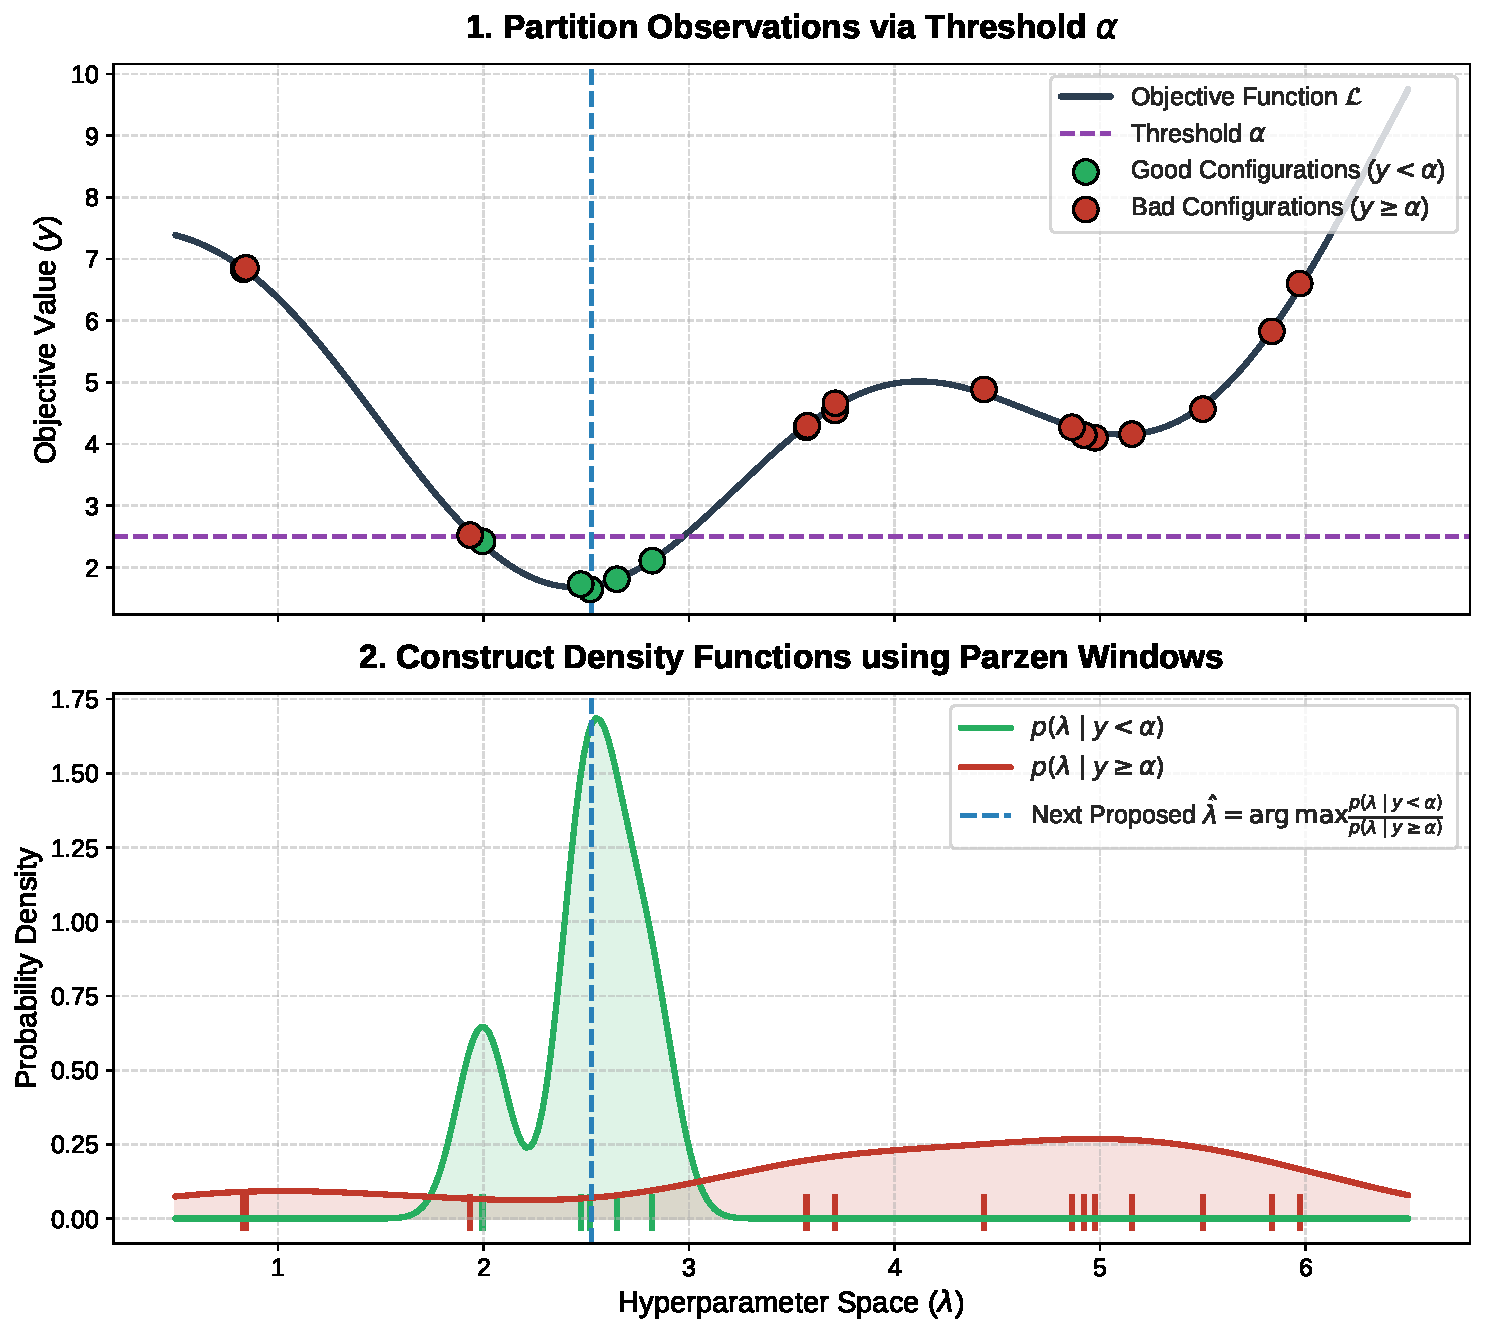
\includegraphics[width=0.8\linewidth]{figures/tpe_mathematical_mechanism.pdf}
\caption[Tree-structured Parzen Estimator]{Mathematical mechanism of the \acf{TPE}. The upper window illustrates the objective function $\mathcal{L}$, where evaluated configurations are partitioned by the threshold $\alpha$. Green points represent promising configurations falling below this threshold, whereas red points indicate suboptimal configurations. The lower window displays the corresponding probability density functions constructed using Parzen windows: $p(\lambda \mid y < \alpha)$ for the good configurations and $p(\lambda \mid y \ge \alpha)$ for the bad configurations. The next hyperparameter configuration to be evaluated is proposed based on these distributions, indicated by the vertical blue dashed line across both plots.}
\label{fig:tpe_illustration}
\end{figure}

\FloatBarrier

\section{Mathematical Details of the Search Space}
\label{app:math_search_space}

This appendix provides the formal mathematical definitions for the \ac{AutoML} search space components introduced in Section \ref{subsec:search_space}.
All definitions are adapted from \textcite{AutoMLHoos} to reflect the fixed training and validation split we used for this work.

\paragraph{Hyperparameter Optimisation.}

Let $A_{\lambda}$ denote a learning algorithm $A$ instantiated with hyperparameter configuration $\lambda \in \Lambda$, where $\Lambda$ is the hyperparameter search space.
Given a dataset $\mathcal{D}$ split into a training set $\mathcal{D}_{train}$ and a validation set $\mathcal{D}_{val}$, the \ac{HPO} objective is defined as Equation \ref{eq:app8},
\begin{equation}
    \lambda^* = \arg\min_{\lambda \in \Lambda} \mathcal{L}(A_{\lambda}, \mathcal{D}_{train}, \mathcal{D}_{val})
    \label{eq:app8}
\end{equation}
where $\mathcal{L}$ represents a validation loss metric. Since evaluating $\mathcal{L}$ requires fully training $A_\lambda$, each function evaluation is expensive, and \ac{HPO} is a black-box optimisation problem.

\paragraph{Model Selection.}
The algorithm selection problem is defined as finding the algorithm $A^* \in \mathcal{A}$ that yields the lowest error on the validation set, as defined per Equation \ref{eq:appx9}.
\begin{equation}
    A^* = \arg\min_{A \in \mathcal{A}} \mathcal{L}(A, \mathcal{D}_{train}, \mathcal{D}_{val})
    \label{eq:appx9}
\end{equation}

\paragraph{CASH Problem.}
Given a set of learning algorithms $\mathcal{A}$, each algorithm $A^{(j)} \in \mathcal{A}$ is associated with a specific hyperparameter configuration space $\Lambda^{(j)}$.
The \ac{CASH} problem is formulated to jointly identify the optimal algorithm $A^*$ and its corresponding optimal hyperparameter configuration $\lambda^*$, as defined per Equation \ref{eq:appx10}:
\begin{equation}
    A^*, \lambda^* = \arg\min_{A^{(j)} \in \mathcal{A}, \lambda \in \Lambda^{(j)}} \mathcal{L}(A^{(j)}_{\lambda}, \mathcal{D}_{train}, \mathcal{D}_{val})
    \label{eq:appx10}
\end{equation}





\FloatBarrier









\section{CTRV--EKF Jacobian Derivation}
\label{app:ctrv-jacobian}

This appendix derives the full Jacobian $\mathbf{A}_k = \partial f /
\partial \mathbf{x}|_{\hat{\mathbf{x}}^+_k}$ of the CTRV transition
function introduced in Eq.~\eqref{eq:ctrv-ekf-f_and_c}. 
The state vector is $\hat{\mathbf{x}}_k = (x_k,\, y_k,\, \dot{x}_k,\, \dot{y}_k,\, \omega_k)^\top$ and $\Delta\psi = \omega_k\,\Delta t$.

\subsection*{Case $|\omega_k| \geq \varepsilon$}

\paragraph{Position rows with respect to $(x_k, y_k)$.}
The new position $x_{k+1} = x_k + g(\dot{x}_k, \dot{y}_k, \omega_k)$ depends on $x_k$
linearly with slope 1, and does not depend on $y_k$. The partial derivatives are defined by Equation~\ref{eq:deriv_pos_xy}.
\begin{equation}
    \frac{\partial x_{k+1}}{\partial x_k} = 1, \quad
    \frac{\partial x_{k+1}}{\partial y_k} = 0, \quad
    \frac{\partial y_{k+1}}{\partial x_k} = 0, \quad
    \frac{\partial y_{k+1}}{\partial y_k} = 1
    \label{eq:deriv_pos_xy}
\end{equation}

\paragraph{Position rows with respect to $(\dot{x}_k, \dot{y}_k)$.}
The arc-length update is given by Equation~\ref{eq:arclength_update}:
\begin{equation}
    x_{k+1} = x_k + \frac{\dot{x}_k\sin\Delta\psi + \dot{y}_k(\cos\Delta\psi - 1)}{\omega_k},\quad
    y_{k+1} = y_k + \frac{\dot{y}_k\sin\Delta\psi - \dot{x}_k(\cos\Delta\psi - 1)}{\omega_k}
    \label{eq:arclength_update}
\end{equation}


 Because both terms appear linearly, differentiation with respect to $\dot{x}_k$ and $\dot{y}_k$ yields Equation~\ref{eq:deriv_pos_vel},:
\begin{equation}
    \frac{\partial x_{k+1}}{\partial \dot{x}_k} = \frac{\sin\Delta\psi}{\omega_k}, \quad
    \frac{\partial x_{k+1}}{\partial \dot{y}_k} = \frac{\cos\Delta\psi - 1}{\omega_k}, \quad
    \frac{\partial y_{k+1}}{\partial \dot{x}_k} = \frac{1 - \cos\Delta\psi}{\omega_k}, \quad
    \frac{\partial y_{k+1}}{\partial \dot{y}_k} = \frac{\sin\Delta\psi}{\omega_k}
    \label{eq:deriv_pos_vel}
\end{equation}

\paragraph{Position rows with respect to $\omega_k$.}
By applying the quotient rule to $x_{k+1} = x_k + u(\omega_k)/\omega_k$, where $u = \dot{x}_k\sin\Delta\psi + \dot{y}_k(\cos\Delta\psi - 1)$ and $\mathrm{d}\Delta\psi/\mathrm{d}\omega_k = \Delta t$, the derivative is obtained as shown in Equation~\ref{eq:deriv_pos_omega}.
\begin{align}
    \frac{\partial x_{k+1}}{\partial \omega_k}
    &= \frac{\omega_k \cdot \frac{\mathrm{d}u}{\mathrm{d}\omega_k} - u}{\omega_k^2}
     = \frac{\Delta t\,(\dot{x}_k\cos\Delta\psi - \dot{y}_k\sin\Delta\psi)\cdot\omega_k
             - \bigl(\dot{x}_k\sin\Delta\psi + \dot{y}_k(\cos\Delta\psi-1)\bigr)}{\omega_k^2}
    \label{eq:deriv_pos_omega}
\end{align}
The numerator factor $\dot{x}_k\cos\Delta\psi - \dot{y}_k\sin\Delta\psi$ corresponds to the rotated velocity $\dot{x}_{k+1}$ from $f$, which results in the compact form defined by Equation~\ref{eq:a15}:
\begin{equation}
    a_{15} = \frac{\Delta\psi\,\dot{x}_{k+1} - \bigl(\dot{x}_k\sin\Delta\psi + \dot{y}_k(\cos\Delta\psi-1)\bigr)}{\omega_k^2}
    \label{eq:a15}
\end{equation}
Analogously, the derivation for $a_{25}$ yields Equation~\ref{eq:a25}:
\begin{equation}
    a_{25} = \frac{\Delta\psi\,\dot{y}_{k+1} - \bigl(\dot{y}_k\sin\Delta\psi - \dot{x}_k(\cos\Delta\psi-1)\bigr)}{\omega_k^2}
    \label{eq:a25}
\end{equation}



\paragraph{Velocity rows with respect to $(\dot{x}_k, \dot{y}_k)$.}
The velocity update is a rotation by $\Delta\psi$, represented by Equation~\ref{eq:vel_rot_mat}.
\begin{equation}
    \begin{pmatrix}\dot{x}_{k+1}\\\dot{y}_{k+1}\end{pmatrix} = \mathbf{R}(\Delta\psi) \begin{pmatrix}\dot{x}_k\\\dot{y}_k\end{pmatrix}, \quad
    \mathbf{R}(\Delta\psi) = \begin{pmatrix}\cos\Delta\psi & -\sin\Delta\psi \\ \sin\Delta\psi &  \cos\Delta\psi\end{pmatrix}
    \label{eq:vel_rot_mat}
\end{equation}
Since the update is linear in $(\dot{x}_k, \dot{y}_k)$, the Jacobian block is
$\mathbf{R}(\Delta\psi)$ itself.

\paragraph{Velocity rows with respect to $\omega_k$.}
Differentiating $\dot{x}_{k+1} = \dot{x}_k\cos\Delta\psi - \dot{y}_k\sin\Delta\psi$
with respect to $\omega_k$, using $\mathrm{d}\Delta\psi/\mathrm{d}\omega_k = \Delta t$, results in Equation~\ref{eq:vel_deriv_omega}.
\begin{equation}
    \frac{\partial \dot{x}_{k+1}}{\partial \omega_k} =
    (-\dot{x}_k\sin\Delta\psi - \dot{y}_k\cos\Delta\psi)\,\Delta t, \qquad
    \frac{\partial \dot{y}_{k+1}}{\partial \omega_k} =
    (\dot{x}_k\cos\Delta\psi - \dot{y}_k\sin\Delta\psi)\,\Delta t
        \label{eq:vel_deriv_omega}
\end{equation}


\paragraph{Turn-rate row.}
Since $\omega_{k+1} = \omega_k$, all partial derivatives are zero except
$\partial\omega_{k+1}/\partial\omega_k = 1$.

\subsection*{Case $|\omega_k| < \varepsilon$: Taylor Approximation}

To avoid division by zero, we substitute:
\begin{equation}
    \sin\Delta\psi \approx \Delta\psi, \qquad
    \cos\Delta\psi \approx 1.
\end{equation}

To avoid division by zero, we apply the Taylor approximations as defined by Equation~\ref{eq:taylor_approx}.
\begin{equation}
    \sin\Delta\psi \approx \Delta\psi, \qquad \cos\Delta\psi \approx 1.
    \label{eq:taylor_approx}
\end{equation}

The position update simplifies to the constant-velocity step
$x_{k+1} \approx x_k + \dot{x}_k\,\Delta t$, $y_{k+1} \approx y_k + \dot{y}_k\,\Delta t$,
while the Jacobian is reduced to the form defined by Equation~\ref{eq:jacobian_taylor}.


\begin{equation}
    \mathbf{A}_k\big|_{|\omega_k|<\varepsilon} =
    \begin{pmatrix}
        1 & 0 & \Delta t & 0 & -\tfrac{1}{2}\dot{y}_k\,\Delta t^2 \\
        0 & 1 & 0 & \Delta t &  \tfrac{1}{2}\dot{x}_k\,\Delta t^2 \\
        0 & 0 & 1 & 0 & -\dot{y}_k\,\Delta t \\
        0 & 0 & 0 & 1 &  \dot{x}_k\,\Delta t \\
        0 & 0 & 0 & 0 & 1
    \end{pmatrix}
    \label{eq:jacobian_taylor}
\end{equation}


%%%%%%%%%%%%%----------------%%%%%%%%%%%%%%%%%%%%----------------------------------CODEBASE--------------------%%%%%%%%%%%%%%%%%%%%%%%%%%%%%%%%%%%%%%%%%%%%%%%%
\chapter{Codebase Overview} 
\label{chap:appendixcodebase}


\begin{figure}[p]
    \centering
    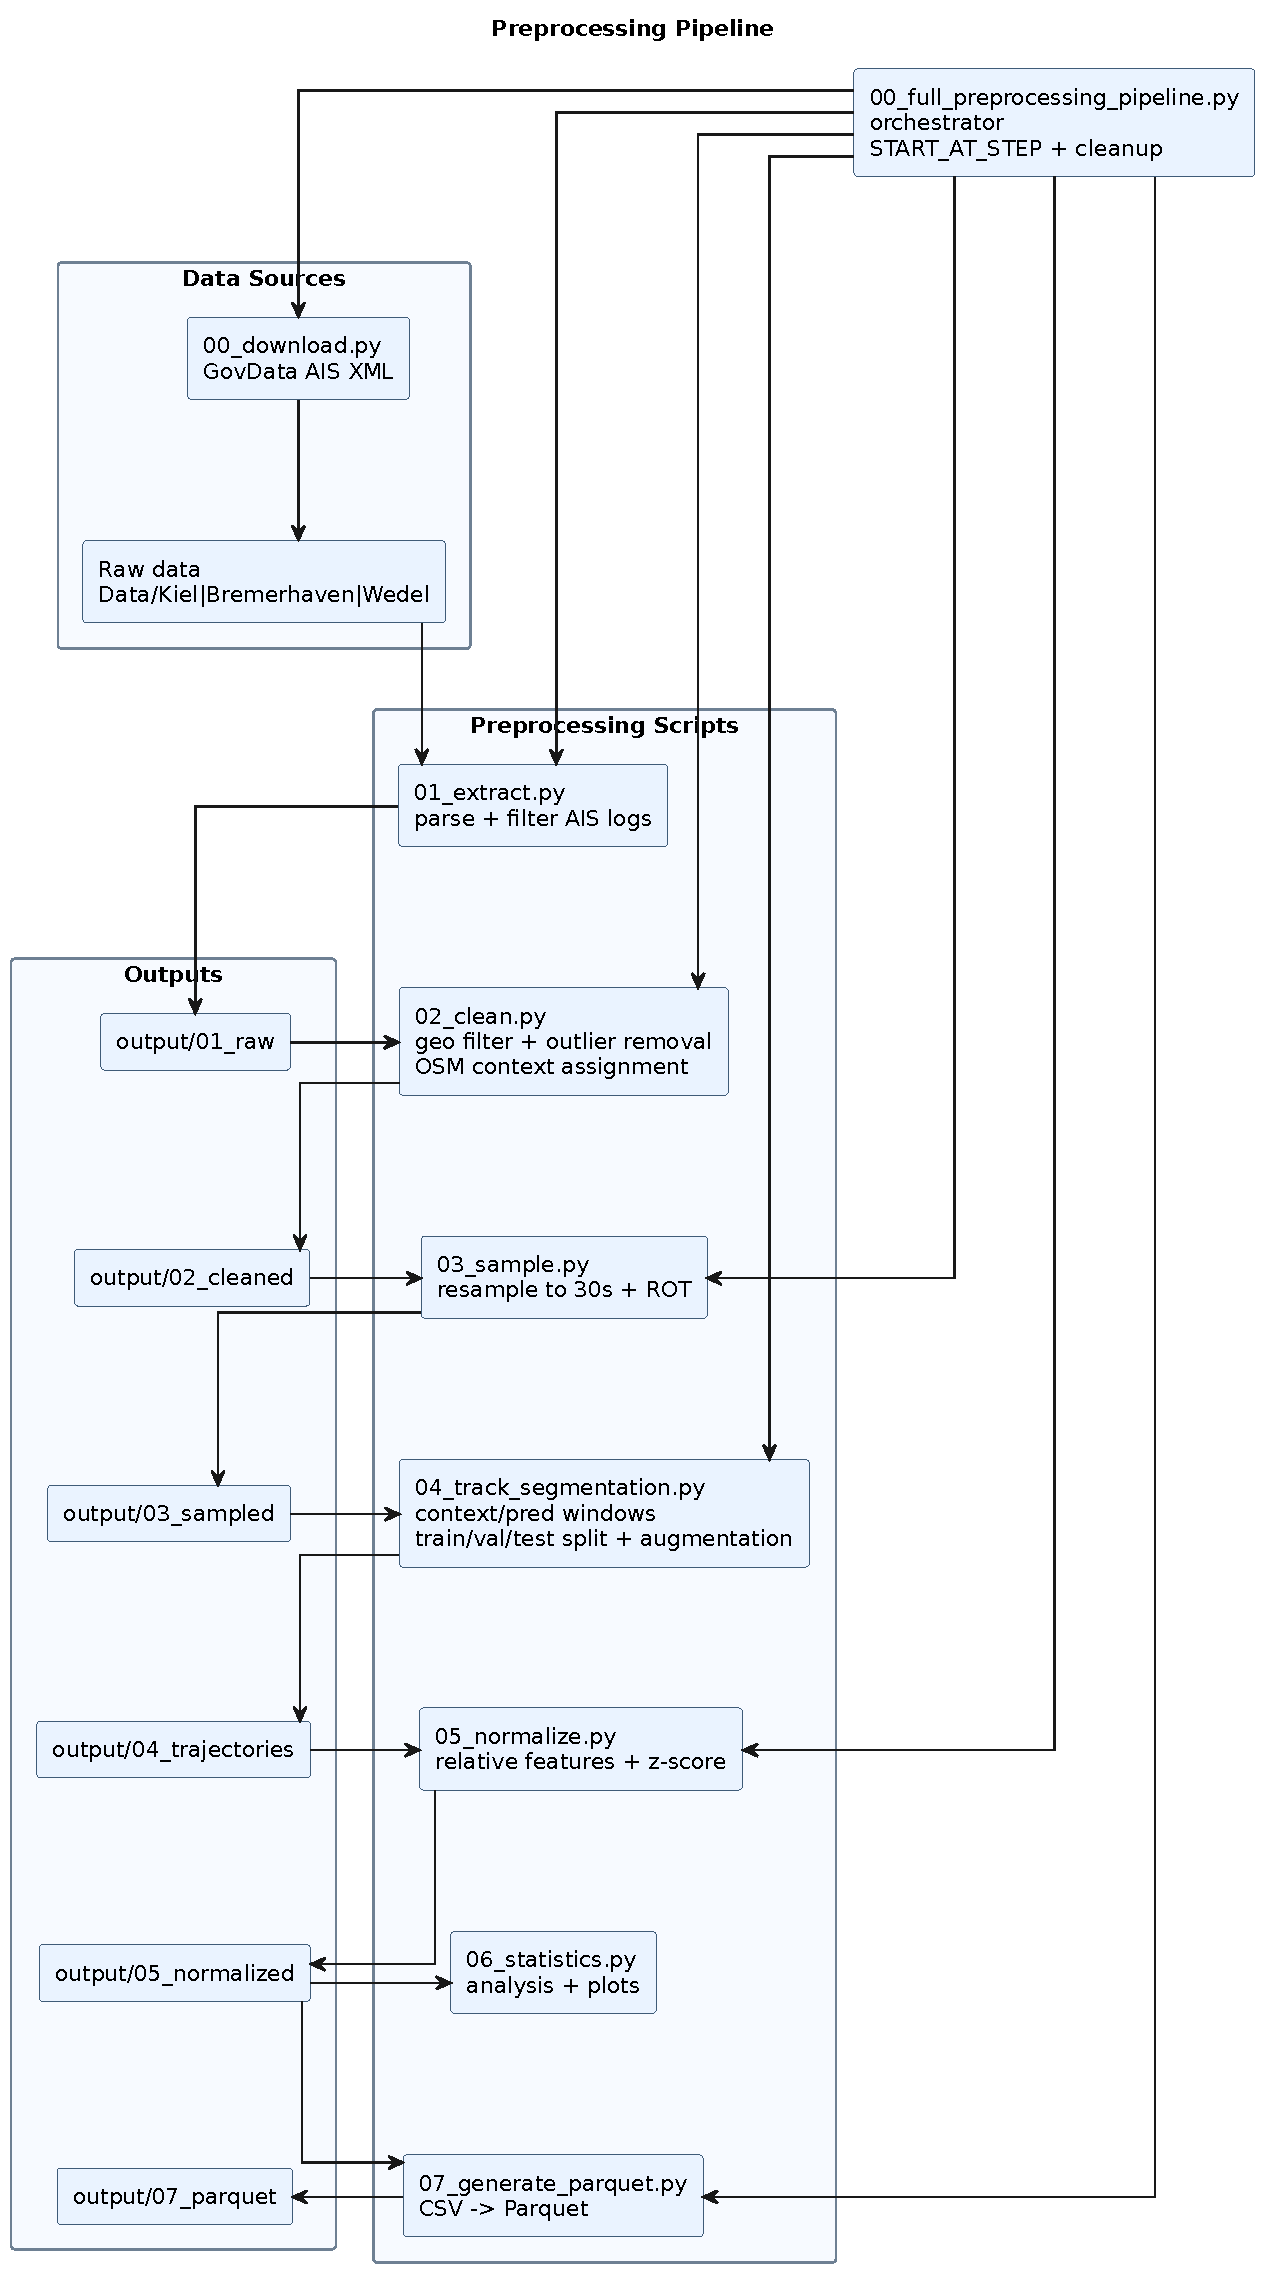
\includegraphics[width=0.75\linewidth]{figures/preprocessing_highlevel.pdf}
    \caption[Code Overview: Preprocessing Pipeline]{%
    \textbf{Preprocessing pipeline file interactions.}
    The pipeline is orchestrated by \texttt{00\_full\_preprocessing\_pipeline.py}, which invokes steps 01--07 sequentially and can resume from any intermediate step via \texttt{START\_AT\_STEP}.
    Raw AIS data is fetched by \texttt{00\_download.py} and stored under \texttt{Data/}.
    Each script reads from the previous output folder and writes into the next:
    \texttt{01\_extract.py} $\to$ \texttt{output/01\_raw} $\to$
    \texttt{02\_clean.py} $\to$ \texttt{output/02\_cleaned} $\to$
    \texttt{03\_sample.py} $\to$ \texttt{output/03\_sampled} $\to$
    \texttt{04\_track\_segmentation.py} $\to$ \texttt{output/04\_trajectories} $\to$
    \texttt{05\_normalize.py} $\to$ \texttt{output/05\_normalized} $\to$
    \texttt{07\_generate\_parquet.py} $\to$ \texttt{output/07\_parquet}.
    \texttt{06\_statistics.py} reads from \texttt{output/05\_normalized} to generate analysis figures and produces no further output folder.

    }    \label{fig:codepreprocessing}
\end{figure}

\clearpage


\begin{sidewaysfigure}
    \centering
    \makebox[0pt]{%symetrical overflow
        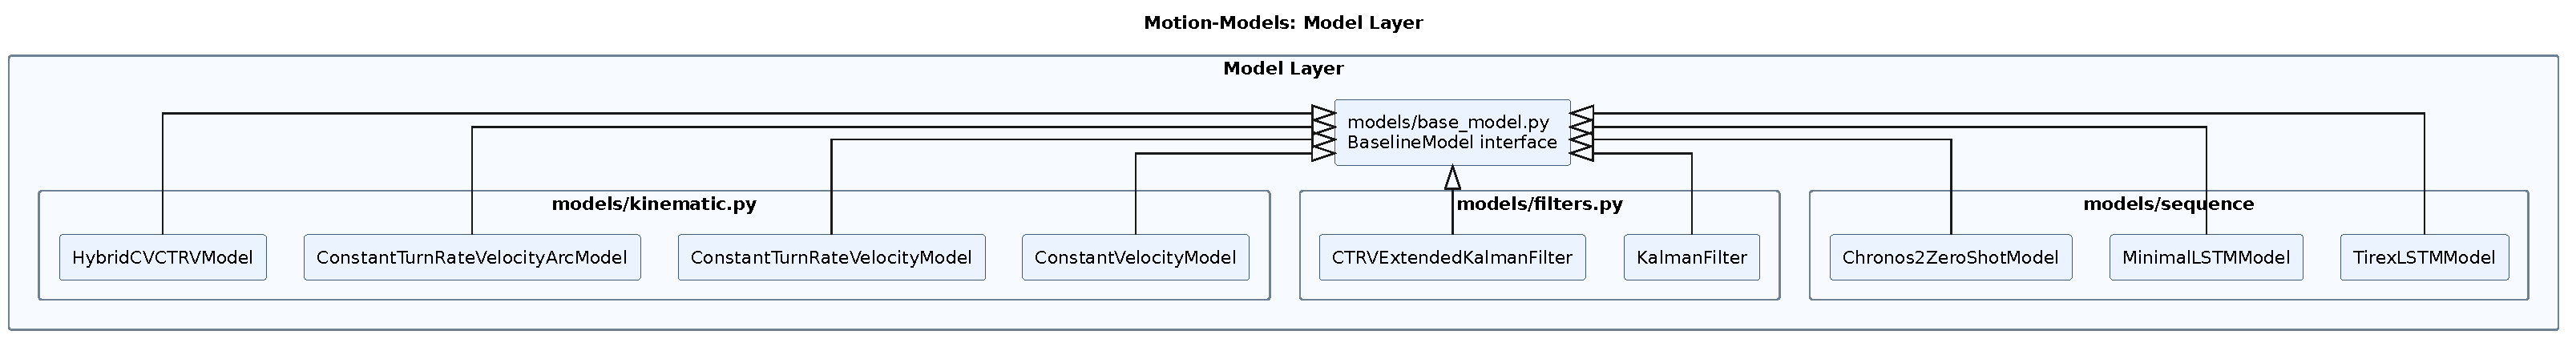
\includegraphics[width=1.18\textheight, keepaspectratio]{figures/models_highlevel.pdf}
    }
    \caption[Code Overview: Model Layer]{%
        \textbf{Model layer class hierarchy.}
        All models inherit from \texttt{BaselineModel} (\texttt{models/base\_model.py}), which defines the common interface used by the evaluation framework: \texttt{predict(context\_df,~n\_pred\_steps)}.
        The \emph{kinematic} group (\texttt{models/kinematic.py}) contains: \texttt{ConstantVelocityModel} (CV), \texttt{ConstantTurnRateVelocityModel} (CTRV), \texttt{ConstantTurnRateVelocityArcModel} (CTRV Arc), and \texttt{HybridCVCTRVModel}, which selects between CV and CTRV per sample based on a rotation-rate threshold.
        The \emph{filter} group (\texttt{models/filters.py}) contains \texttt{KalmanFilter} and \texttt{CTRVExtendedKalmanFilter}.
        The \emph{sequence} group (\texttt{models/sequence/}) contains data-driven models: \texttt{TirexLSTMModel} (TiRex), \texttt{MinimalLSTMModel (LSTM)}, and \texttt{Chronos2ZeroShotModel} (Chronos-2).
    }    \label{fig:codemodels}
\end{sidewaysfigure}
\clearpage

\begin{sidewaysfigure}
    \centering
    \makebox[0pt]{%
        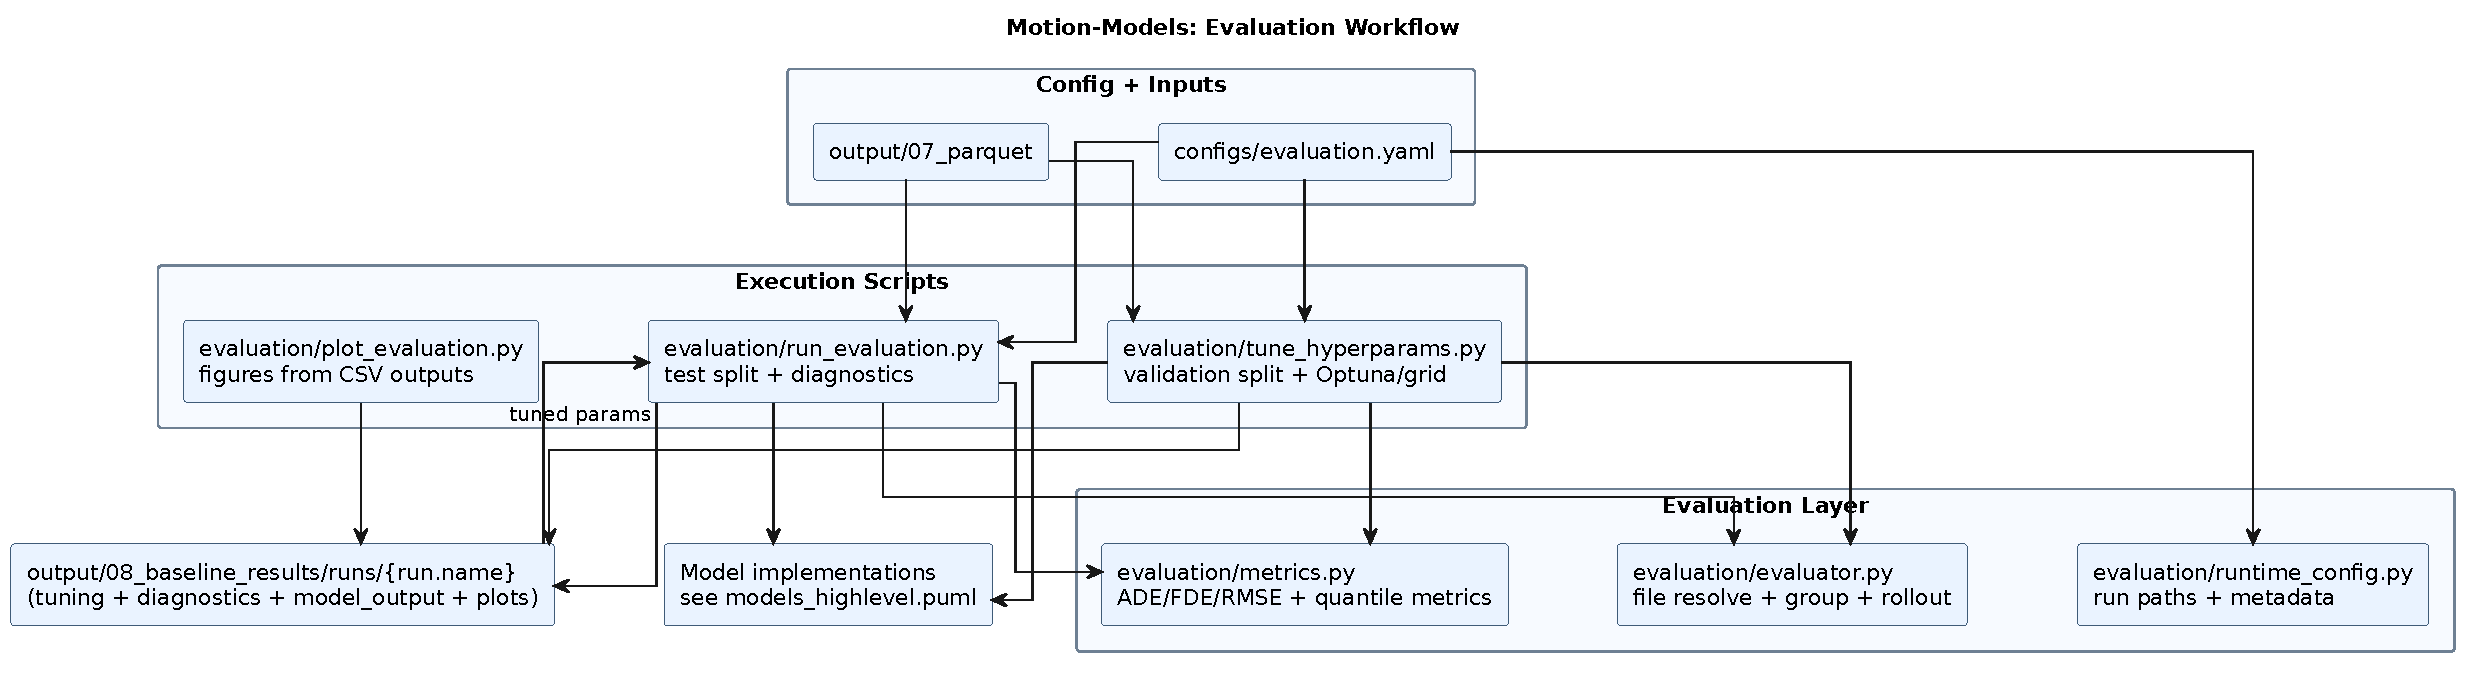
\includegraphics[width=1.18\linewidth, keepaspectratio]{figures/models_evaluation_highlevel.pdf}
    }
    %\caption[Code Overview: Evaluation]{Model Evaluation}
    \caption[Code Overview: Evaluation Workflow]{
        \textbf{Evaluation workflow file and module interactions.}
        The evaluation framework takes two external inputs: the Parquet dataset produced by the preprocessing pipeline (\texttt{output/07\_parquet}) and a YAML configuration file (\texttt{configs/evaluation.yaml}) that specifies enabled models, hyperparameter search spaces, and output paths.
        \texttt{evaluation/runtime\_config.py} resolves run-specific paths and metadata from the configuration.
        \textbf{Tuning} (\texttt{tune\_hyperparams.py}) operates exclusively on the validation split: single-parameter models (CV, CTRV, CTRV Arc, TiRex LSTM) are tuned via exhaustive grid search in parallel worker processes, while multi-parameter models (Hybrid, Kalman, CTRV EKF) are tuned with Optuna TPE.
        Tuning results are written as CSV files under \texttt{output/08\_baseline\_results/runs/\{run.name\}/tuning/}.
        \textbf{Final evaluation} (\texttt{run\_evaluation.py}) reads the tuned parameters and evaluates all enabled models on the test split, writing per-file and per-month diagnostic tables and optional per-model prediction exports to the same run folder.
        Both scripts delegate to \texttt{evaluation/evaluator.py} for file resolution, track grouping, model rollout, and metric aggregation, and to \texttt{evaluation/metrics.py} for computing ADE, FDE, RMSE, and quantile metrics.
        \texttt{evaluation/plot\_evaluation.py} reads the saved CSV outputs to generate all evaluation figures independently of the evaluation runs themselves.
    }
    \label{fig:codeevaluation}
\end{sidewaysfigure}
\clearpage

\begin{comment} dont include it ws
    \chapter{Thesis Advertisement}\begin{figure}
    \centering
    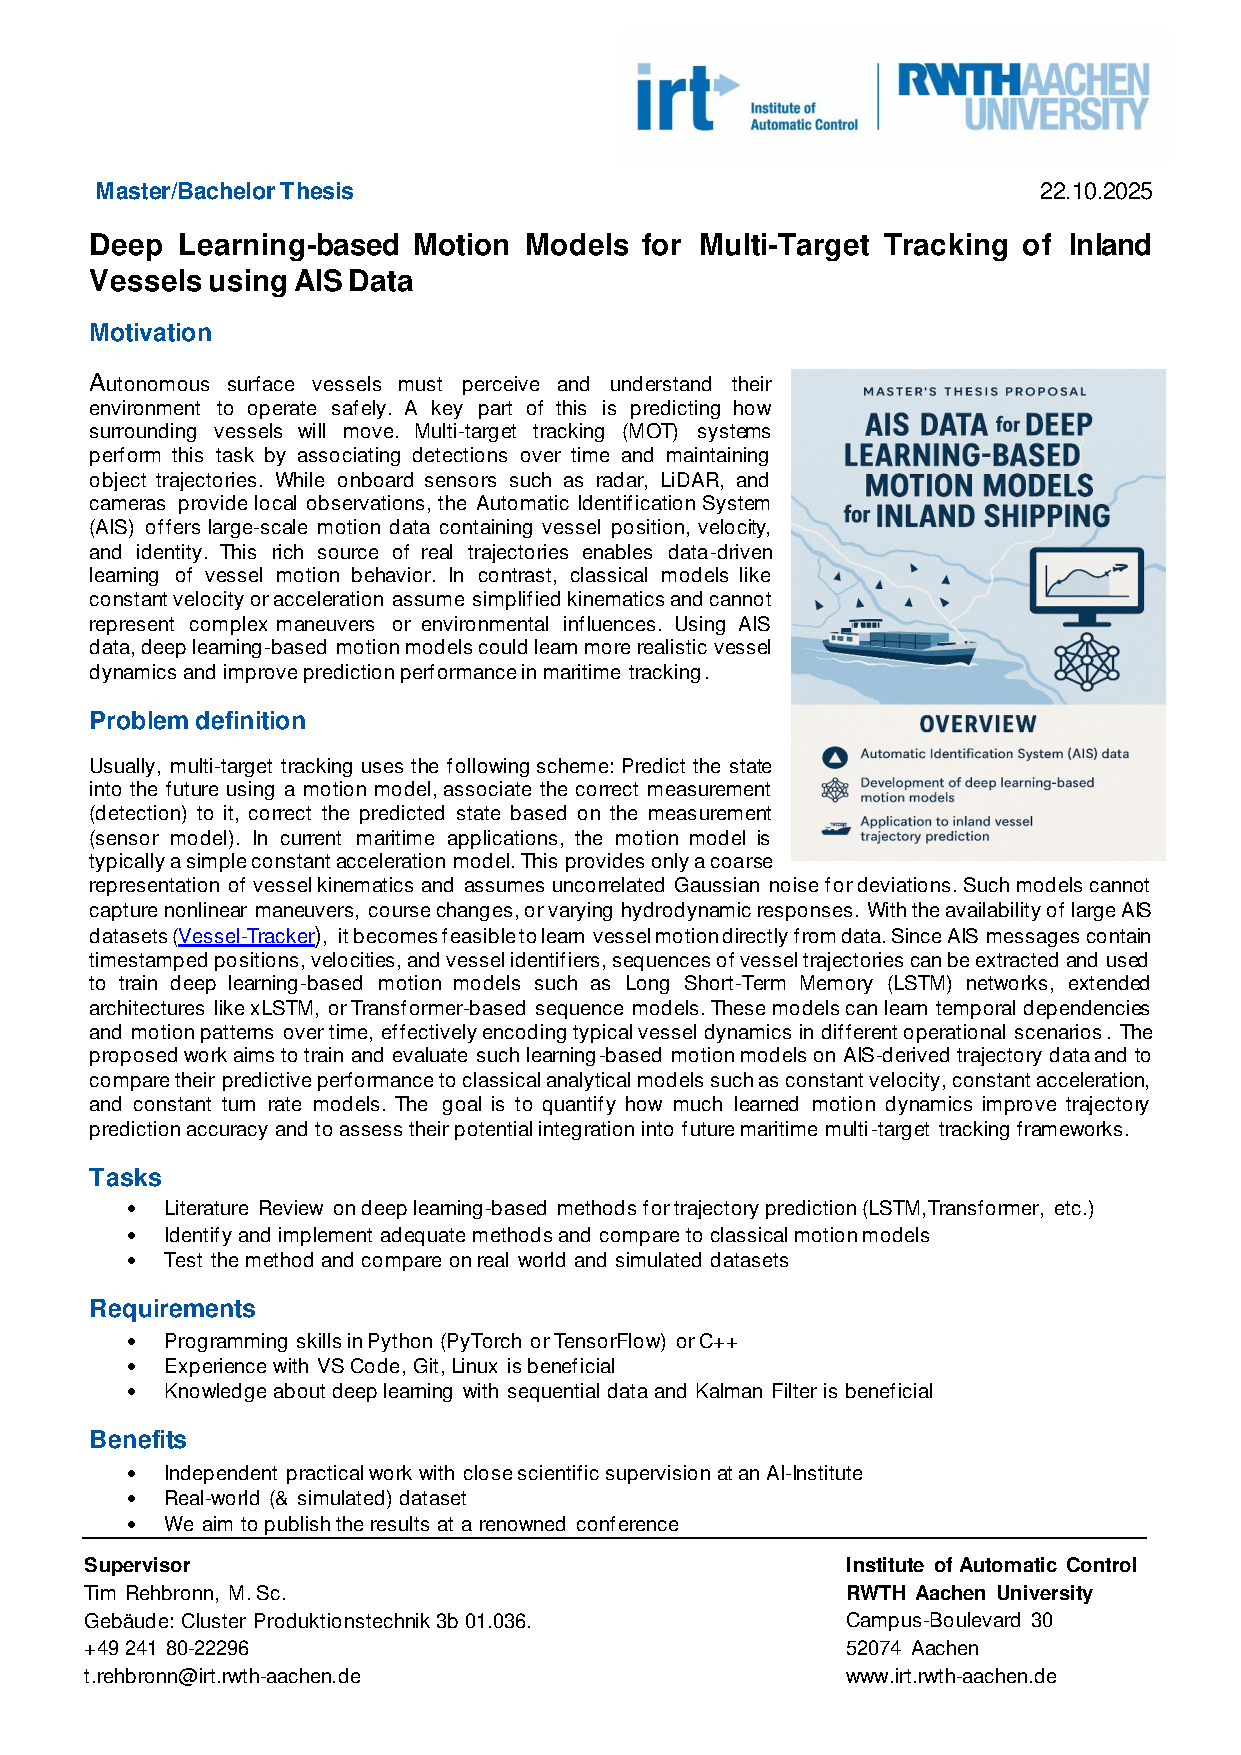
\includegraphics[width=1\linewidth]{ausschreibung_irt.pdf}
    \label{fig:auschschreibung_irt}
\end{figure}

\clearpage
\end{comment}

